% Options for packages loaded elsewhere
\PassOptionsToPackage{unicode}{hyperref}
\PassOptionsToPackage{hyphens}{url}
%
\documentclass[
  ignorenonframetext,
]{article}
\usepackage{pgfpages}
\setbeamertemplate{caption}[numbered]
\setbeamertemplate{caption label separator}{: }
\setbeamercolor{caption name}{fg=normal text.fg}
\beamertemplatenavigationsymbolsempty
% Prevent slide breaks in the middle of a paragraph
\widowpenalties 1 10000
\raggedbottom
\setbeamertemplate{part page}{
  \centering
  \begin{beamercolorbox}[sep=16pt,center]{part title}
    \usebeamerfont{part title}\insertpart\par
  \end{beamercolorbox}
}
\setbeamertemplate{section page}{
  \centering
  \begin{beamercolorbox}[sep=12pt,center]{part title}
    \usebeamerfont{section title}\insertsection\par
  \end{beamercolorbox}
}
\setbeamertemplate{subsection page}{
  \centering
  \begin{beamercolorbox}[sep=8pt,center]{part title}
    \usebeamerfont{subsection title}\insertsubsection\par
  \end{beamercolorbox}
}
\AtBeginPart{
  \frame{\partpage}
}
\AtBeginSection{
  \ifbibliography
  \else
    \frame{\sectionpage}
  \fi
}
\AtBeginSubsection{
  \frame{\subsectionpage}
}
\usepackage{lmodern}
\usepackage{amssymb,amsmath}
\usepackage{ifxetex,ifluatex}
\ifnum 0\ifxetex 1\fi\ifluatex 1\fi=0 % if pdftex
  \usepackage[T1]{fontenc}
  \usepackage[utf8]{inputenc}
  \usepackage{textcomp} % provide euro and other symbols
\else % if luatex or xetex
  \usepackage{unicode-math}
  \defaultfontfeatures{Scale=MatchLowercase}
  \defaultfontfeatures[\rmfamily]{Ligatures=TeX,Scale=1}
\fi
% Use upquote if available, for straight quotes in verbatim environments
\IfFileExists{upquote.sty}{\usepackage{upquote}}{}
\IfFileExists{microtype.sty}{% use microtype if available
  \usepackage[]{microtype}
  \UseMicrotypeSet[protrusion]{basicmath} % disable protrusion for tt fonts
}{}
\makeatletter
\@ifundefined{KOMAClassName}{% if non-KOMA class
  \IfFileExists{parskip.sty}{%
    \usepackage{parskip}
  }{% else
    \setlength{\parindent}{0pt}
    \setlength{\parskip}{6pt plus 2pt minus 1pt}}
}{% if KOMA class
  \KOMAoptions{parskip=half}}
\makeatother
\usepackage{xcolor}
\IfFileExists{xurl.sty}{\usepackage{xurl}}{} % add URL line breaks if available
\IfFileExists{bookmark.sty}{\usepackage{bookmark}}{\usepackage{hyperref}}
\hypersetup{
  pdftitle={Using bookdown with Beamer},
  pdfauthor={Marta Ferreira e Pedro Magalhães},
  hidelinks,
  pdfcreator={LaTeX via pandoc}}
\urlstyle{same} % disable monospaced font for URLs
\geometry{margin=2.5cm}
\newif\ifbibliography
\usepackage{color}
\usepackage{fancyvrb}
\newcommand{\VerbBar}{|}
\newcommand{\VERB}{\Verb[commandchars=\\\{\}]}
\DefineVerbatimEnvironment{Highlighting}{Verbatim}{commandchars=\\\{\}}
% Add ',fontsize=\small' for more characters per line
\usepackage{framed}
\definecolor{shadecolor}{RGB}{248,248,248}
\newenvironment{Shaded}{\begin{snugshade}}{\end{snugshade}}
\newcommand{\AlertTok}[1]{\textcolor[rgb]{0.94,0.16,0.16}{#1}}
\newcommand{\AnnotationTok}[1]{\textcolor[rgb]{0.56,0.35,0.01}{\textbf{\textit{#1}}}}
\newcommand{\AttributeTok}[1]{\textcolor[rgb]{0.77,0.63,0.00}{#1}}
\newcommand{\BaseNTok}[1]{\textcolor[rgb]{0.00,0.00,0.81}{#1}}
\newcommand{\BuiltInTok}[1]{#1}
\newcommand{\CharTok}[1]{\textcolor[rgb]{0.31,0.60,0.02}{#1}}
\newcommand{\CommentTok}[1]{\textcolor[rgb]{0.56,0.35,0.01}{\textit{#1}}}
\newcommand{\CommentVarTok}[1]{\textcolor[rgb]{0.56,0.35,0.01}{\textbf{\textit{#1}}}}
\newcommand{\ConstantTok}[1]{\textcolor[rgb]{0.00,0.00,0.00}{#1}}
\newcommand{\ControlFlowTok}[1]{\textcolor[rgb]{0.13,0.29,0.53}{\textbf{#1}}}
\newcommand{\DataTypeTok}[1]{\textcolor[rgb]{0.13,0.29,0.53}{#1}}
\newcommand{\DecValTok}[1]{\textcolor[rgb]{0.00,0.00,0.81}{#1}}
\newcommand{\DocumentationTok}[1]{\textcolor[rgb]{0.56,0.35,0.01}{\textbf{\textit{#1}}}}
\newcommand{\ErrorTok}[1]{\textcolor[rgb]{0.64,0.00,0.00}{\textbf{#1}}}
\newcommand{\ExtensionTok}[1]{#1}
\newcommand{\FloatTok}[1]{\textcolor[rgb]{0.00,0.00,0.81}{#1}}
\newcommand{\FunctionTok}[1]{\textcolor[rgb]{0.00,0.00,0.00}{#1}}
\newcommand{\ImportTok}[1]{#1}
\newcommand{\InformationTok}[1]{\textcolor[rgb]{0.56,0.35,0.01}{\textbf{\textit{#1}}}}
\newcommand{\KeywordTok}[1]{\textcolor[rgb]{0.13,0.29,0.53}{\textbf{#1}}}
\newcommand{\NormalTok}[1]{#1}
\newcommand{\OperatorTok}[1]{\textcolor[rgb]{0.81,0.36,0.00}{\textbf{#1}}}
\newcommand{\OtherTok}[1]{\textcolor[rgb]{0.56,0.35,0.01}{#1}}
\newcommand{\PreprocessorTok}[1]{\textcolor[rgb]{0.56,0.35,0.01}{\textit{#1}}}
\newcommand{\RegionMarkerTok}[1]{#1}
\newcommand{\SpecialCharTok}[1]{\textcolor[rgb]{0.00,0.00,0.00}{#1}}
\newcommand{\SpecialStringTok}[1]{\textcolor[rgb]{0.31,0.60,0.02}{#1}}
\newcommand{\StringTok}[1]{\textcolor[rgb]{0.31,0.60,0.02}{#1}}
\newcommand{\VariableTok}[1]{\textcolor[rgb]{0.00,0.00,0.00}{#1}}
\newcommand{\VerbatimStringTok}[1]{\textcolor[rgb]{0.31,0.60,0.02}{#1}}
\newcommand{\WarningTok}[1]{\textcolor[rgb]{0.56,0.35,0.01}{\textbf{\textit{#1}}}}
\usepackage{longtable,booktabs}
\usepackage{caption}
% Make caption package work with longtable
\makeatletter
\def\fnum@table{\tablename~\thetable}
\makeatother
\setlength{\emergencystretch}{3em} % prevent overfull lines
\providecommand{\tightlist}{%
  \setlength{\itemsep}{0pt}\setlength{\parskip}{0pt}}
\setcounter{secnumdepth}{5}
%----------------------------------------------------------------------------------------
%	REQUIRED PACKAGES
%
% pdfpages:(http://mirrors.up.pt/pub/CTAN/macros/latex/contrib/pdfpages/pdfpages.pdf)
% geometry: (https://www.overleaf.com/learn/latex/Page_size_and_margins)
% fancyhdr: (https://www.overleaf.com/learn/latex/Headers_and_footers)
% xcolor: (https://www.overleaf.com/learn/latex/Using_colours_in_LaTeX)
% titlesec: https://www.overleaf.com/learn/latex/Sections_and_chapters
%----------------------------------------------------------------------------------------

\usepackage{pdfpages} %allows the introduction of pdf pages 
\usepackage{fancyhdr} %changes headers and footers
\usepackage{xcolor} %Lets set different colors for the document
\usepackage{titlesec} %customizes chapters(book) and sections(article)
\usepackage{tikz}
\usepackage{fontspec} %customizes fonts
\usepackage{graphicx} %add graphical elements
\usepackage{background} %customizes documents backgrounds
\usepackage{lastpage}
\usepackage{caption} % allows image caption costumization
\usepackage{blindtext}
\usepackage[most]{tcolorbox}
\tcbuselibrary{skins}
\usepackage{multicol} % allows more than one column on text
\usepackage{enumitem} % Allows to change lists %>% 
\usepackage[default]{opensans}
\usepackage{setspace}\setstretch{1.25}
\usepackage{float}
\floatplacement{figure}{H}
%\usepackage{setspace}\singlespacing

%----------------------------------------------------------------------------------------
%	FONTS FORMAT
%----------------------------------------------------------------------------------------

\setmainfont[SizeFeatures={Size=10}]{Open Sans}

%----------------------------------------------------------------------------------------
%	DOCUMENT COLORS
%----------------------------------------------------------------------------------------

\definecolor{DarkPurple}{HTML}{680c62}
\definecolor{MediumPurple}{HTML}{a8139d}
\definecolor{LightPurple}{HTML}{c26cf0}
\definecolor{Grey}{HTML}{bfbfbf}
\definecolor{lightGreen}{HTML}{ddeedd}
\definecolor{mediumGreen}{HTML}{77bb77}

\definecolor{DarkGray}{HTML}{403D3C}
\definecolor{AtomicGreen}{HTML}{10FF10}

%----------------------------------------------------------------------------------------
%	SECTION FORMAT
%----------------------------------------------------------------------------------------

\titleformat{\section}[block]
  {\titlerule\addvspace{4pt}\normalfont\fontsize{12}{12}\bfseries}
  {\thesection\enspace}{0pt}{}[\vspace{2pt}\titlerule]

\titleformat*{\section}{\color{DarkGray}\fontsize{16}{16}\normalfont\bfseries}
\titleformat*{\subsection}{\color{DarkGray}\fontsize{12}{12}\normalfont\bfseries}
\titleformat*{\subsubsection}{\color{AtomicGreen}\fontsize{10}{10}\normalfont\bfseries}

\titlespacing*{\section}{0pt}{30pt}{50pt}
\titlespacing*{\subsection}{0pt}{40pt}{10pt}

%----------------------------------------------------------------------------------------
%	CUSTOM HEADER AND FOOTER
%----------------------------------------------------------------------------------------

\pagestyle{fancy}
\fancyhf{} %clear all headers and footer fields
%\fancyhead[RO,RE]{\textcolor{DarkGray}{math.marketing}}
\fancyhead[LO,LE]{\textcolor{DarkGray}{\thepage}}
\renewcommand{\headrulewidth}{0pt} %Eliminates header row that is part of the default


\backgroundsetup{
  scale=1.3,
  opacity=1,
  angle=0,
  position=current page.south,
  hshift=0pt, %-27
  vshift=20pt,
  contents={%
  \small\sffamily%
  \begin{minipage}{1\textwidth}
  
\includegraphics[scale=0.5]{theme/images/footer.png}
  \end{minipage}%
  }
}

%----------------------------------------------------------------------------------------
%	CUSTOM IMAGE FORMATING
%----------------------------------------------------------------------------------------

\captionsetup[figure]{name=Fig.}

%----------------------------------------------------------------------------------------
%	COVER PAGE
%----------------------------------------------------------------------------------------

\AtBeginDocument{\let\maketitle\relax}

%----------------------------------------------------------------------------------------
%	NEW COMMANDS
%-------------------------------------------------------------------------------------

% http://texdoc.net/texmf-dist/doc/latex/tcolorbox/tcolorbox.pdf

\newcommand{\impactBox}[2]{
  \begin{tcolorbox}[width=\textwidth,
  fonttitle = \sffamily\bfseries\large, 
  colframe={mediumGreen},
  colback={lightGreen},
  title={#1},
  sharp corners]  
  \textsc{#2}
  \end{tcolorbox} 
}

\newcommand{\attentionBox}[1]{
  \begin{tcolorbox}[fonttitle = \sffamily\bfseries\large,
  bicolor,
  sidebyside,
  lefthand width=0.5cm,
  sharp corners,
  boxrule=.4pt,
  colback=yellow!30,
  colbacklower=yellow!20]
    \includegraphics[scale=5]{theme/images/attention-sign.png}
  \tcblower
    \textsc{#1}%
  \end{tcolorbox}
}
\usepackage[]{natbib}
\bibliographystyle{plainnat}

\title{Using bookdown with Beamer}
\subtitle{Machine Learning}
\author{Marta Ferreira e Pedro Magalhães}
\date{18/04/2022}

\begin{document}
\NoBgThispage %does not apply background

\includepdf{theme/images/cover.pdf}
\frame{\titlepage}



\begin{frame}
  \tableofcontents[hideallsubsections]
\end{frame}
\begin{frame}

\end{frame}

\begin{frame}[fragile]{Introduction}
\protect\hypertarget{introduction}{}
This projects aims at comparing the performance of several Machine Learning models (ML models) under different data contexts.

To achieve our goal we stacked against each other pairs of different models using Synthetic Datasets represents often polarizing and extreme situations and therefore exposing the main ``decision'' characteristics of each model.

The focus will be solely on classification problems and models will be compared againts each other using Accuracy and Area under the Roc Curve (AUC ROC) as metrics. Since we have full control over the dataset distributuion, the optimal Bayes Boundary willbe used as baseline

\begin{block}{Project structure}
\protect\hypertarget{project-structure}{}
This project is organized in the following way:

\begin{enumerate}
\item
  An introduction containing general assumptions and how to reproduce the results,
\item
  A chapter for each model pair containing the sythetic data rules, the bayes optimal boundary (BOB), a small models explanation and rational for each dataset, model fit and metrics as well as the prediction area and discussion of the results,
\item
  An overall conclusion
\end{enumerate}
\end{block}

\begin{block}{Approaches and Assumptions}
\protect\hypertarget{approaches-and-assumptions}{}
Throughtout this project the following assumptions were made and approaches were used:

\begin{itemize}
\item
  Dependent variables (target) are of date type \texttt{factor} and all Independent variables (features) are of type \texttt{numeric},
\item
  Since the datasets are syntheticly generated, no pre-processing was made,
\item
  Datasets were built using statistical distributions and/or classification rules which may have no resemblance to reality,
\item
  To the extant it is possible a dataset was created using a binomial categorical variable and a two features,
\item
  For the sake of molde comparing, the default hyperparameter value were used. This are provided by \texttt{Parsnip\ R\ package} without post-processing and hyperparameter optimzation. It is possible, although unlikely, that a different package or under different hyperparameters could result different conclusions,
\item
  For calculating metrics a crossvalidatios with 10 folds and no repetition was used.
\end{itemize}
\end{block}

\begin{block}{How to run and reproduce the conclusions}
\protect\hypertarget{how-to-run-and-reproduce-the-conclusions}{}

\end{block}
\end{frame}

\begin{frame}[fragile]{logistic vs knn}
\protect\hypertarget{logistic-vs-knn}{}
\begin{block}{Dataset definition}
\protect\hypertarget{dataset-definition}{}
When comparing a Logistic regression model agains a Nearest Neighbour model we are comparing a highly biased and a very flexible approach. While a logostic regression assumes a linear border between both classes, NN makes no assumptions and and relies on local information (by k neighbours) to predict a class.

Given the base assumption of a linear boundary by logistic regression, a model whose border differs, substantially from a line we expect will performe badly. On the other hand the lack of linearity won't an issue for knn.

Therefore, we built two datasets with 1000 observations from a \texttt{Uniform\ Distribution}, one with a classification provided by a linear model of \(X1 >= X2\) and a narrow quadratic function \(abs(1,2 * X_{1} - 5)^2 + 2\).

\begin{Shaded}
\begin{Highlighting}[]
\NormalTok{decision\_fun\_linear }\OtherTok{\textless{}{-}} \ControlFlowTok{function}\NormalTok{(x1, x2)\{}
\NormalTok{  res }\OtherTok{\textless{}{-}} \FunctionTok{ifelse}\NormalTok{(x2 }\SpecialCharTok{\textgreater{}=}\NormalTok{ x1, }\DecValTok{1}\NormalTok{, }\DecValTok{0}\NormalTok{)}
  \FunctionTok{return}\NormalTok{(res)}
\NormalTok{\}}

\NormalTok{decision\_fun\_quadratic }\OtherTok{\textless{}{-}} \ControlFlowTok{function}\NormalTok{(x1, x2)\{}
\NormalTok{  res }\OtherTok{\textless{}{-}} \FunctionTok{ifelse}\NormalTok{(x2 }\SpecialCharTok{\textgreater{}=} \FunctionTok{abs}\NormalTok{( (}\FloatTok{1.2} \SpecialCharTok{*}\NormalTok{ x1 }\SpecialCharTok{{-}} \DecValTok{5}\NormalTok{)}\SpecialCharTok{\^{}}\DecValTok{2} \SpecialCharTok{+} \DecValTok{2}\NormalTok{ ), }\DecValTok{1}\NormalTok{, }\DecValTok{0}\NormalTok{)}
  \FunctionTok{return}\NormalTok{(res)}
\NormalTok{\}}

\NormalTok{dataset\_linear }\OtherTok{\textless{}{-}} \FunctionTok{dataset\_gen\_unif}\NormalTok{(}\AttributeTok{class\_fun =}\NormalTok{ decision\_fun\_linear, }\AttributeTok{size =} \DecValTok{1000}\NormalTok{)}
\end{Highlighting}
\end{Shaded}

\begin{verbatim}
## Warning: The `x` argument of `as_tibble.matrix()` must have unique column names if `.name_repair` is omitted as of tibble 2.0.0.
## Using compatibility `.name_repair`.
## This warning is displayed once every 8 hours.
## Call `lifecycle::last_lifecycle_warnings()` to see where this warning was generated.
\end{verbatim}

\begin{Shaded}
\begin{Highlighting}[]
\NormalTok{dataset\_quadratic }\OtherTok{\textless{}{-}} \FunctionTok{dataset\_gen\_unif}\NormalTok{(}\AttributeTok{class\_fun =}\NormalTok{ decision\_fun\_quadratic, }\AttributeTok{size =} \DecValTok{1000}\NormalTok{)}

\FunctionTok{grid.arrange}\NormalTok{(}
\NormalTok{  dataset\_linear}\SpecialCharTok{$}\NormalTok{border\_plot, }
\NormalTok{  dataset\_quadratic}\SpecialCharTok{$}\NormalTok{border\_plot, }
  \AttributeTok{nrow =} \DecValTok{1}\NormalTok{,}
  \AttributeTok{top =} \StringTok{"Synthetic Generated Datasets"}\NormalTok{,}
  \AttributeTok{bottom =}\NormalTok{ grid}\SpecialCharTok{::}\FunctionTok{textGrob}\NormalTok{(}
    \StringTok{"Dashed line represent optimal bayes decision border"}\NormalTok{,}
    \AttributeTok{gp =}\NormalTok{ grid}\SpecialCharTok{::}\FunctionTok{gpar}\NormalTok{(}\AttributeTok{fontface =} \DecValTok{3}\NormalTok{, }\AttributeTok{fontsize =} \DecValTok{9}\NormalTok{)}
\NormalTok{    )}
\NormalTok{  )}
\end{Highlighting}
\end{Shaded}

\begin{center}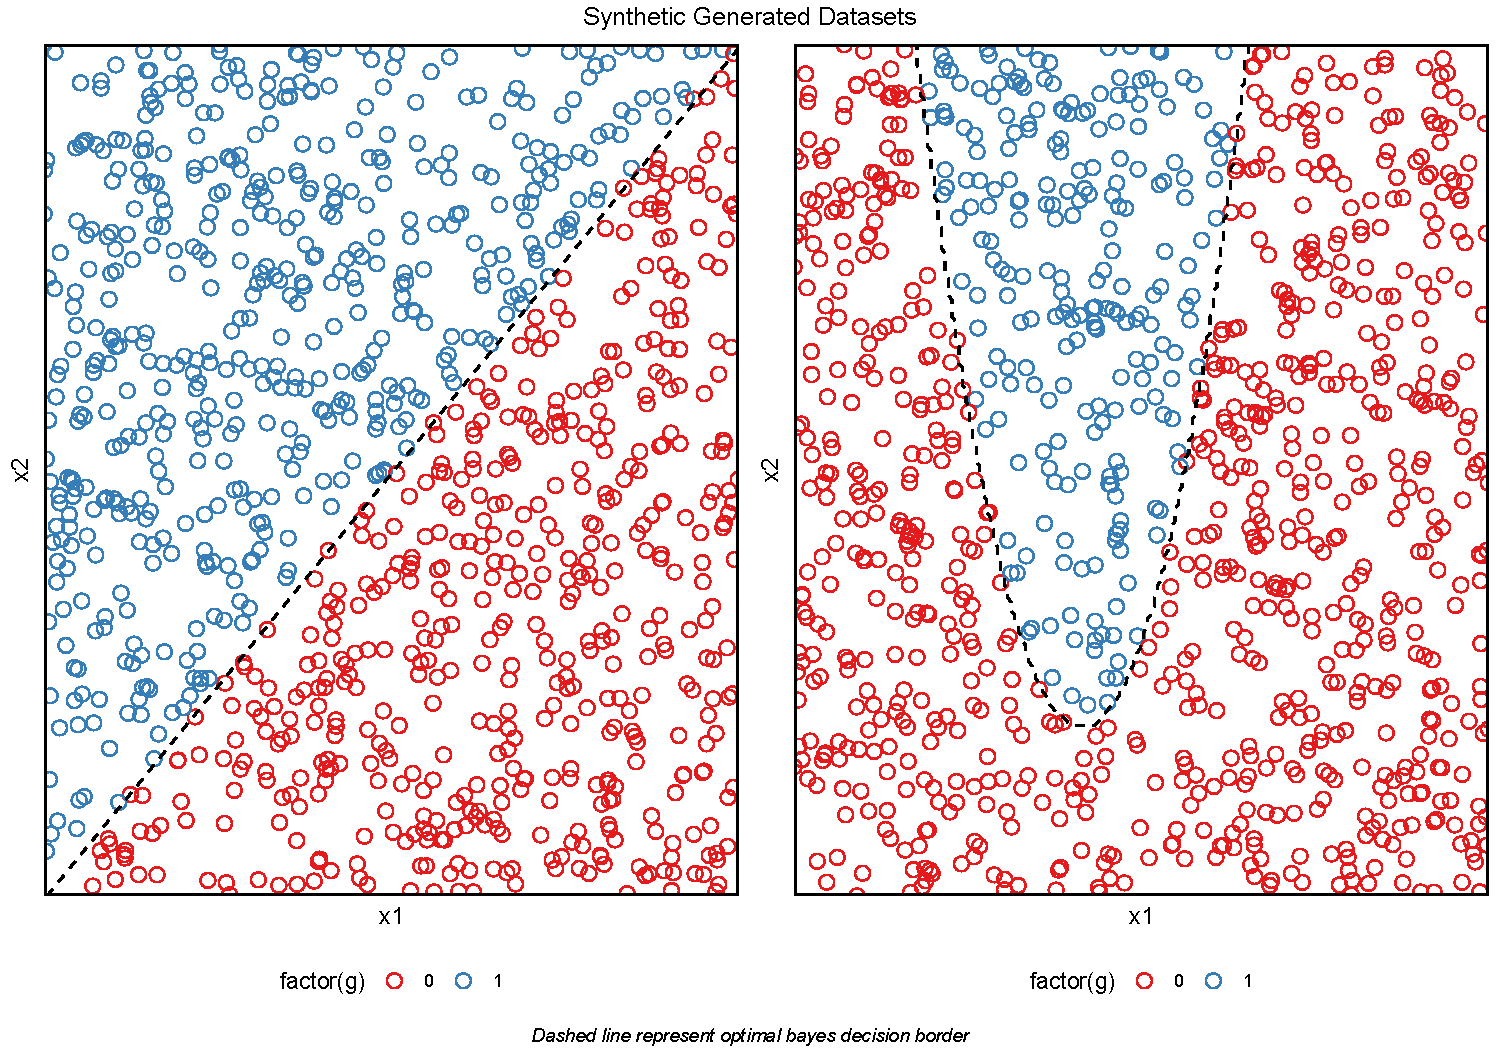
\includegraphics{_main_files/figure-beamer/unnamed-chunk-5-1} \end{center}
\end{block}

\begin{block}{Model fitting}
\protect\hypertarget{model-fitting}{}
Each dataset was divided on training and test dataset using a 80/20 split.

\begin{Shaded}
\begin{Highlighting}[]
\CommentTok{\# 0. Separate test and train}

\NormalTok{data\_linear }\OtherTok{\textless{}{-}}\NormalTok{ dataset\_linear}\SpecialCharTok{$}\NormalTok{dataset}
\NormalTok{data\_linear}\SpecialCharTok{$}\NormalTok{g }\OtherTok{\textless{}{-}} \FunctionTok{factor}\NormalTok{(data\_linear}\SpecialCharTok{$}\NormalTok{g)}

\NormalTok{split }\OtherTok{\textless{}{-}} \FunctionTok{initial\_split}\NormalTok{(data\_linear, }\AttributeTok{prop =} \FloatTok{0.8}\NormalTok{)}

\NormalTok{train\_data\_linear }\OtherTok{\textless{}{-}} \FunctionTok{training}\NormalTok{(split)}
\NormalTok{test\_data\_linear }\OtherTok{\textless{}{-}} \FunctionTok{testing}\NormalTok{(split)}




\NormalTok{data\_quadratic }\OtherTok{\textless{}{-}}\NormalTok{ dataset\_quadratic}\SpecialCharTok{$}\NormalTok{dataset}
\NormalTok{data\_quadratic}\SpecialCharTok{$}\NormalTok{g }\OtherTok{\textless{}{-}} \FunctionTok{factor}\NormalTok{(data\_quadratic}\SpecialCharTok{$}\NormalTok{g)}

\NormalTok{split }\OtherTok{\textless{}{-}} \FunctionTok{initial\_split}\NormalTok{(data\_quadratic, }\AttributeTok{prop =} \FloatTok{0.8}\NormalTok{)}

\NormalTok{train\_data\_quadratic }\OtherTok{\textless{}{-}} \FunctionTok{training}\NormalTok{(split)}
\NormalTok{test\_data\_quadratic }\OtherTok{\textless{}{-}} \FunctionTok{testing}\NormalTok{(split)}
\end{Highlighting}
\end{Shaded}

\begin{block}{Logistic regression}
\protect\hypertarget{logistic-regression}{}
\begin{Shaded}
\begin{Highlighting}[]
\DocumentationTok{\#\# Create workflow}

\DocumentationTok{\#\#\# Logistic regression {-}{-}{-}{-}{-}{-}{-}{-}{-}{-}{-}{-}{-}{-}{-}{-}{-}{-}{-}{-}{-}{-}{-}{-}{-}}

 
\CommentTok{\# 1. specify the model}
\NormalTok{logistic\_reg\_glm\_spec }\OtherTok{\textless{}{-}}
  \FunctionTok{logistic\_reg}\NormalTok{(}\AttributeTok{mode =} \StringTok{"classification"}\NormalTok{) }\SpecialCharTok{\%\textgreater{}\%}
  \FunctionTok{set\_engine}\NormalTok{(}\StringTok{\textquotesingle{}glm\textquotesingle{}}\NormalTok{, }\AttributeTok{family =} \StringTok{"binomial"}\NormalTok{) }

\CommentTok{\# 2. preprocessing }
\NormalTok{preprocess }\OtherTok{\textless{}{-}} 
  \FunctionTok{recipe}\NormalTok{(g }\SpecialCharTok{\textasciitilde{}}\NormalTok{ x1 }\SpecialCharTok{+}\NormalTok{ x2 , }\AttributeTok{data =}\NormalTok{ train\_data\_linear)}
  
\CommentTok{\# 3, Buildworkflow}
\NormalTok{logit\_wflow }\OtherTok{\textless{}{-}} 
  \FunctionTok{workflow}\NormalTok{() }\SpecialCharTok{\%\textgreater{}\%} 
  \FunctionTok{add\_model}\NormalTok{(logistic\_reg\_glm\_spec) }\SpecialCharTok{\%\textgreater{}\%} 
  \FunctionTok{add\_recipe}\NormalTok{(preprocess)}

\CommentTok{\# 4. Fit model}
\NormalTok{fit\_control }\OtherTok{\textless{}{-}} \FunctionTok{control\_resamples}\NormalTok{(}\AttributeTok{save\_pred =} \ConstantTok{TRUE}\NormalTok{, }\AttributeTok{save\_workflow =} \ConstantTok{TRUE}\NormalTok{)}

\NormalTok{folds\_linear }\OtherTok{\textless{}{-}} \FunctionTok{vfold\_cv}\NormalTok{(train\_data\_linear, }\AttributeTok{v =} \DecValTok{10}\NormalTok{)}
\NormalTok{folds\_quadratic }\OtherTok{\textless{}{-}} \FunctionTok{vfold\_cv}\NormalTok{(train\_data\_quadratic, }\AttributeTok{v =} \DecValTok{10}\NormalTok{)}


\NormalTok{logit\_metrics\_linear }\OtherTok{\textless{}{-}} 
\NormalTok{  logit\_wflow }\SpecialCharTok{\%\textgreater{}\%} 
  \FunctionTok{fit\_resamples}\NormalTok{(folds\_linear, }\AttributeTok{verbose =} \ConstantTok{TRUE}\NormalTok{, }\AttributeTok{control =}\NormalTok{ fit\_control)}
\end{Highlighting}
\end{Shaded}

\begin{verbatim}
## Warning: The `...` are not used in this function but one or more objects were
## passed: 'verbose'
\end{verbatim}

\begin{verbatim}
## ! Fold01: preprocessor 1/1, model 1/1: glm.fit: algorithm did not converge, glm.fi...
\end{verbatim}

\begin{verbatim}
## ! Fold02: preprocessor 1/1, model 1/1: glm.fit: algorithm did not converge, glm.fi...
\end{verbatim}

\begin{verbatim}
## ! Fold03: preprocessor 1/1, model 1/1: glm.fit: algorithm did not converge, glm.fi...
\end{verbatim}

\begin{verbatim}
## ! Fold04: preprocessor 1/1, model 1/1: glm.fit: algorithm did not converge, glm.fi...
\end{verbatim}

\begin{verbatim}
## ! Fold05: preprocessor 1/1, model 1/1: glm.fit: algorithm did not converge, glm.fi...
\end{verbatim}

\begin{verbatim}
## ! Fold06: preprocessor 1/1, model 1/1: glm.fit: algorithm did not converge, glm.fi...
\end{verbatim}

\begin{verbatim}
## ! Fold07: preprocessor 1/1, model 1/1: glm.fit: algorithm did not converge, glm.fi...
\end{verbatim}

\begin{verbatim}
## ! Fold08: preprocessor 1/1, model 1/1: glm.fit: algorithm did not converge, glm.fi...
\end{verbatim}

\begin{verbatim}
## ! Fold09: preprocessor 1/1, model 1/1: glm.fit: algorithm did not converge, glm.fi...
\end{verbatim}

\begin{verbatim}
## ! Fold10: preprocessor 1/1, model 1/1: glm.fit: algorithm did not converge, glm.fi...
\end{verbatim}

\begin{Shaded}
\begin{Highlighting}[]
\NormalTok{logit\_metrics\_quadratic }\OtherTok{\textless{}{-}} 
\NormalTok{  logit\_wflow }\SpecialCharTok{\%\textgreater{}\%} 
  \FunctionTok{fit\_resamples}\NormalTok{(folds\_quadratic, }\AttributeTok{verbose =} \ConstantTok{TRUE}\NormalTok{, }\AttributeTok{control =}\NormalTok{ fit\_control)}
\end{Highlighting}
\end{Shaded}

\begin{verbatim}
## Warning: The `...` are not used in this function but one or more objects were
## passed: 'verbose'
\end{verbatim}

\begin{Shaded}
\begin{Highlighting}[]
\CommentTok{\# 5. Performance metrics over the validation set}
\NormalTok{logit\_metrics\_linear }\OtherTok{\textless{}{-}} \FunctionTok{collect\_metrics}\NormalTok{(logit\_metrics\_linear, }\AttributeTok{summarize =} \ConstantTok{FALSE}\NormalTok{)}
\NormalTok{logit\_metrics\_quadratic }\OtherTok{\textless{}{-}} \FunctionTok{collect\_metrics}\NormalTok{(logit\_metrics\_quadratic, }\AttributeTok{summarize =} \ConstantTok{FALSE}\NormalTok{)}


\CommentTok{\# 6. Fits final model}
\NormalTok{logit\_linear\_fit }\OtherTok{\textless{}{-}} 
\NormalTok{  logit\_wflow }\SpecialCharTok{\%\textgreater{}\%} 
  \FunctionTok{fit}\NormalTok{(train\_data\_linear)}
\end{Highlighting}
\end{Shaded}

\begin{verbatim}
## Warning: glm.fit: algorithm did not converge
\end{verbatim}

\begin{verbatim}
## Warning: glm.fit: fitted probabilities numerically 0 or 1 occurred
\end{verbatim}

\begin{Shaded}
\begin{Highlighting}[]
\NormalTok{logit\_linear\_model }\OtherTok{\textless{}{-}} \FunctionTok{extract\_fit\_parsnip}\NormalTok{(logit\_linear\_fit)}

\NormalTok{logit\_quadratic\_fit }\OtherTok{\textless{}{-}} 
\NormalTok{  logit\_wflow }\SpecialCharTok{\%\textgreater{}\%} 
  \FunctionTok{fit}\NormalTok{(train\_data\_quadratic)}

\NormalTok{logit\_quadratic\_model }\OtherTok{\textless{}{-}} \FunctionTok{extract\_fit\_parsnip}\NormalTok{(logit\_quadratic\_fit)}
\end{Highlighting}
\end{Shaded}
\end{block}

\begin{block}{KNN}
\protect\hypertarget{knn}{}
\begin{verbatim}
## Warning: The `...` are not used in this function but one or more objects were passed: 'verbose'
## The `...` are not used in this function but one or more objects were passed: 'verbose'
\end{verbatim}
\end{block}
\end{block}

\begin{block}{Compare results}
\protect\hypertarget{compare-results}{}
The plots below show the resulting decision bondaries

\begin{center}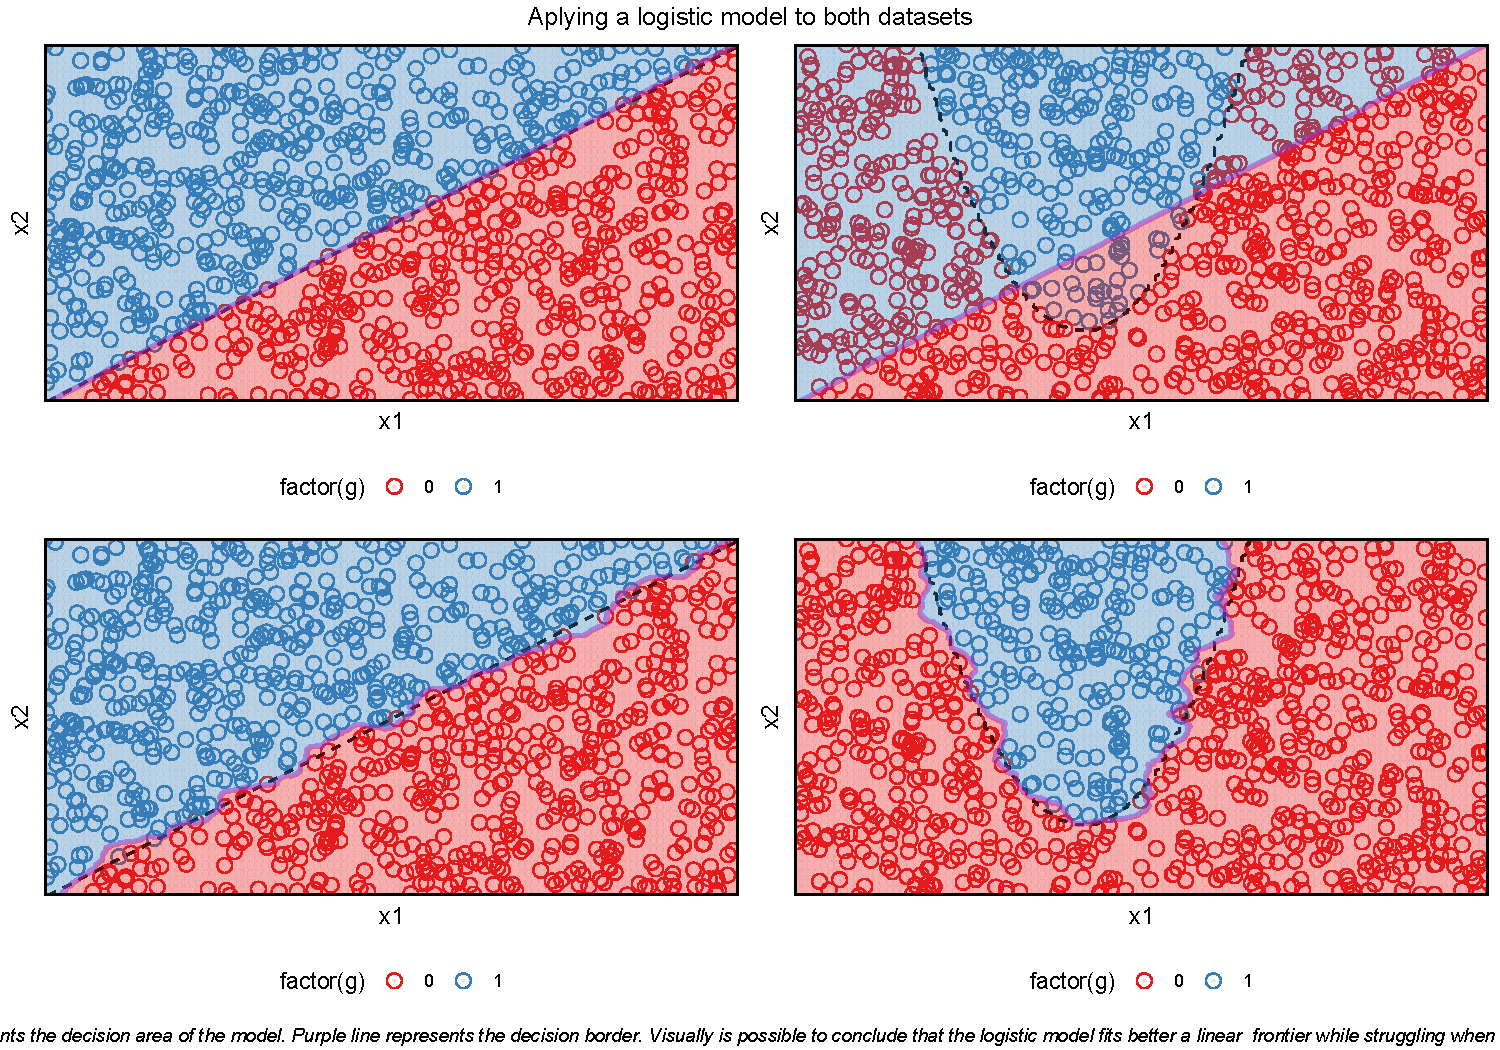
\includegraphics{_main_files/figure-beamer/unnamed-chunk-13-1} \end{center}

The plots shows the evolution of key metrics over crossvalidation trainning

\begin{center}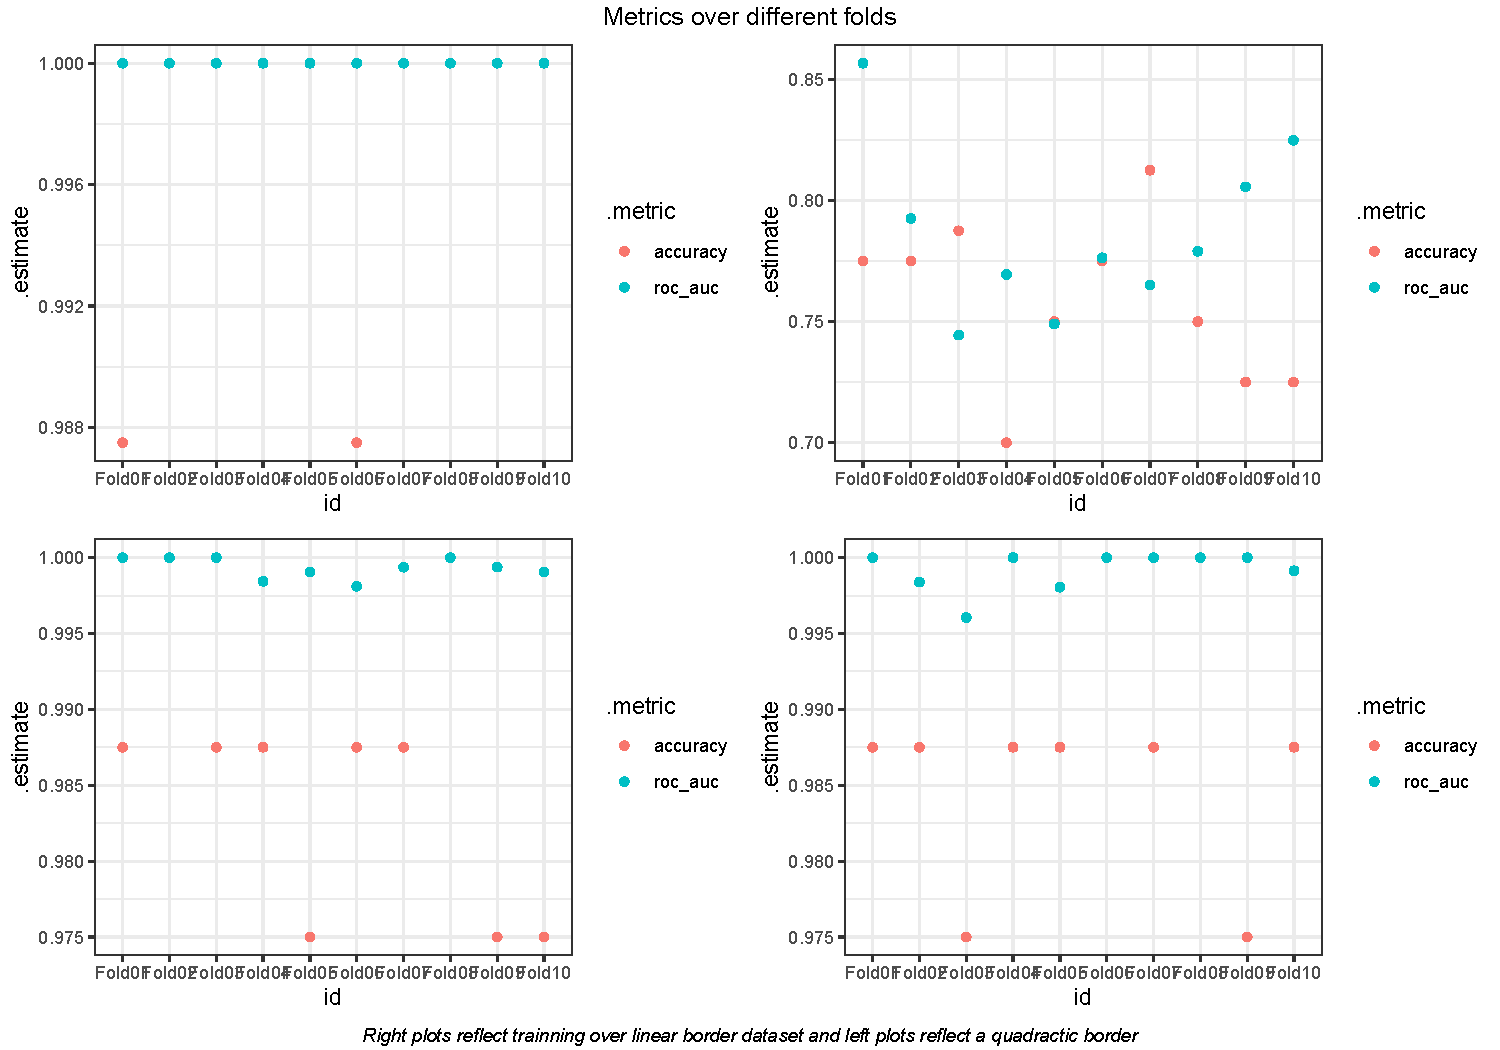
\includegraphics{_main_files/figure-beamer/unnamed-chunk-14-1} \end{center}

The plots show the metrics between different models

\begin{center}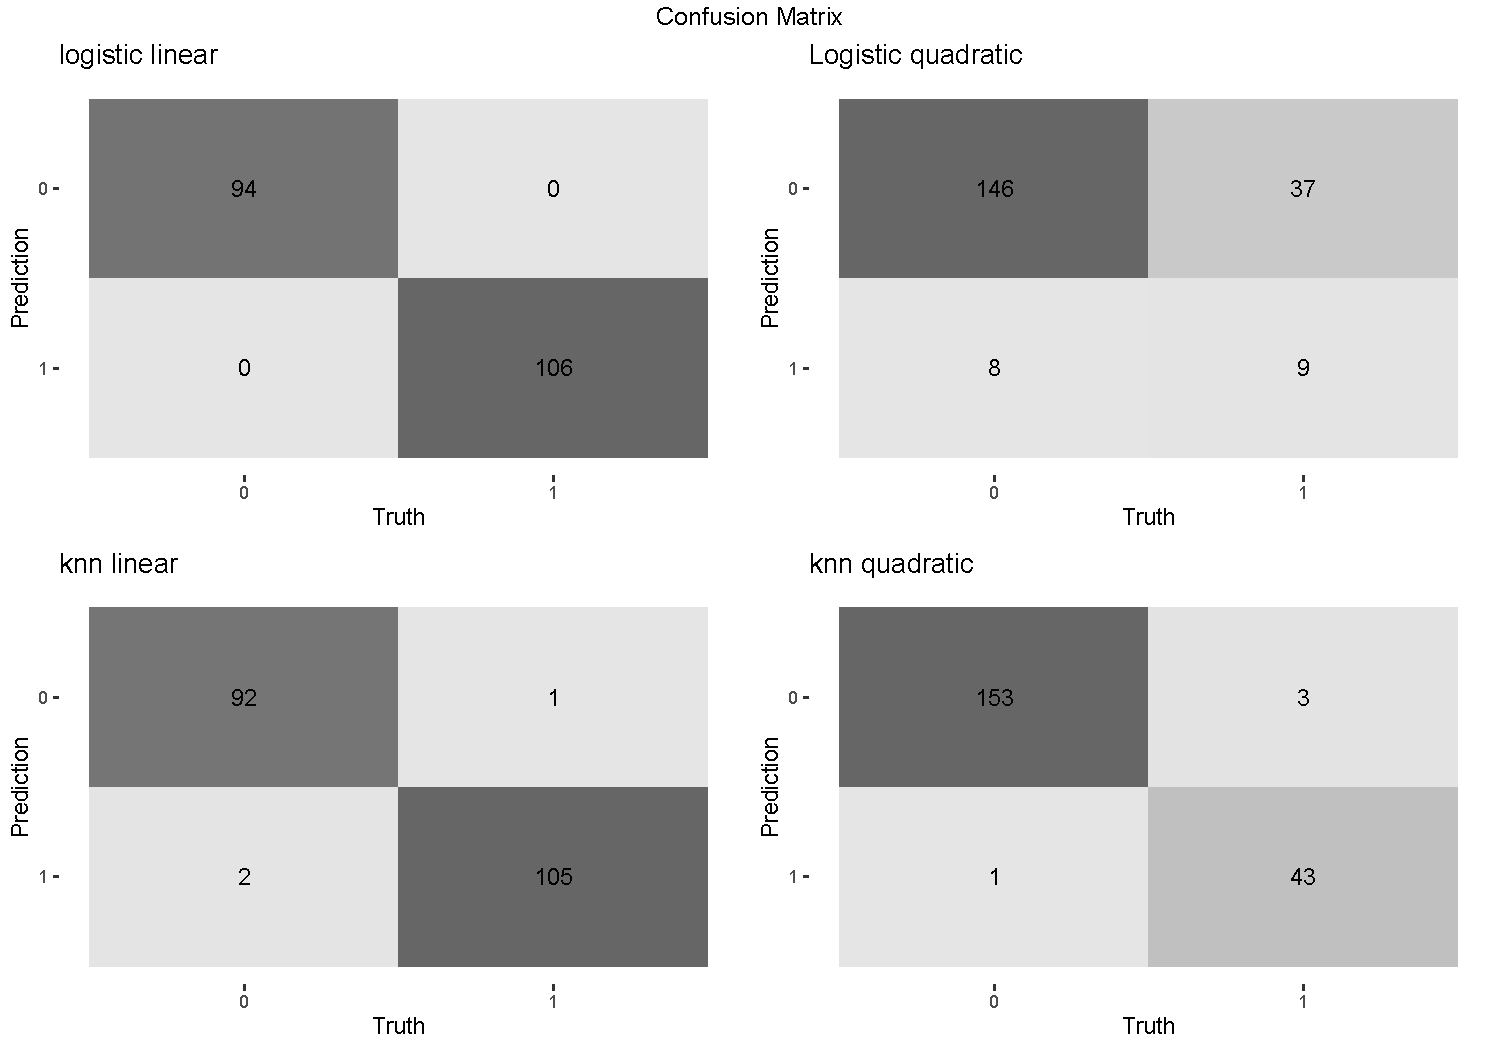
\includegraphics{_main_files/figure-beamer/unnamed-chunk-15-1} \end{center}

\begin{center}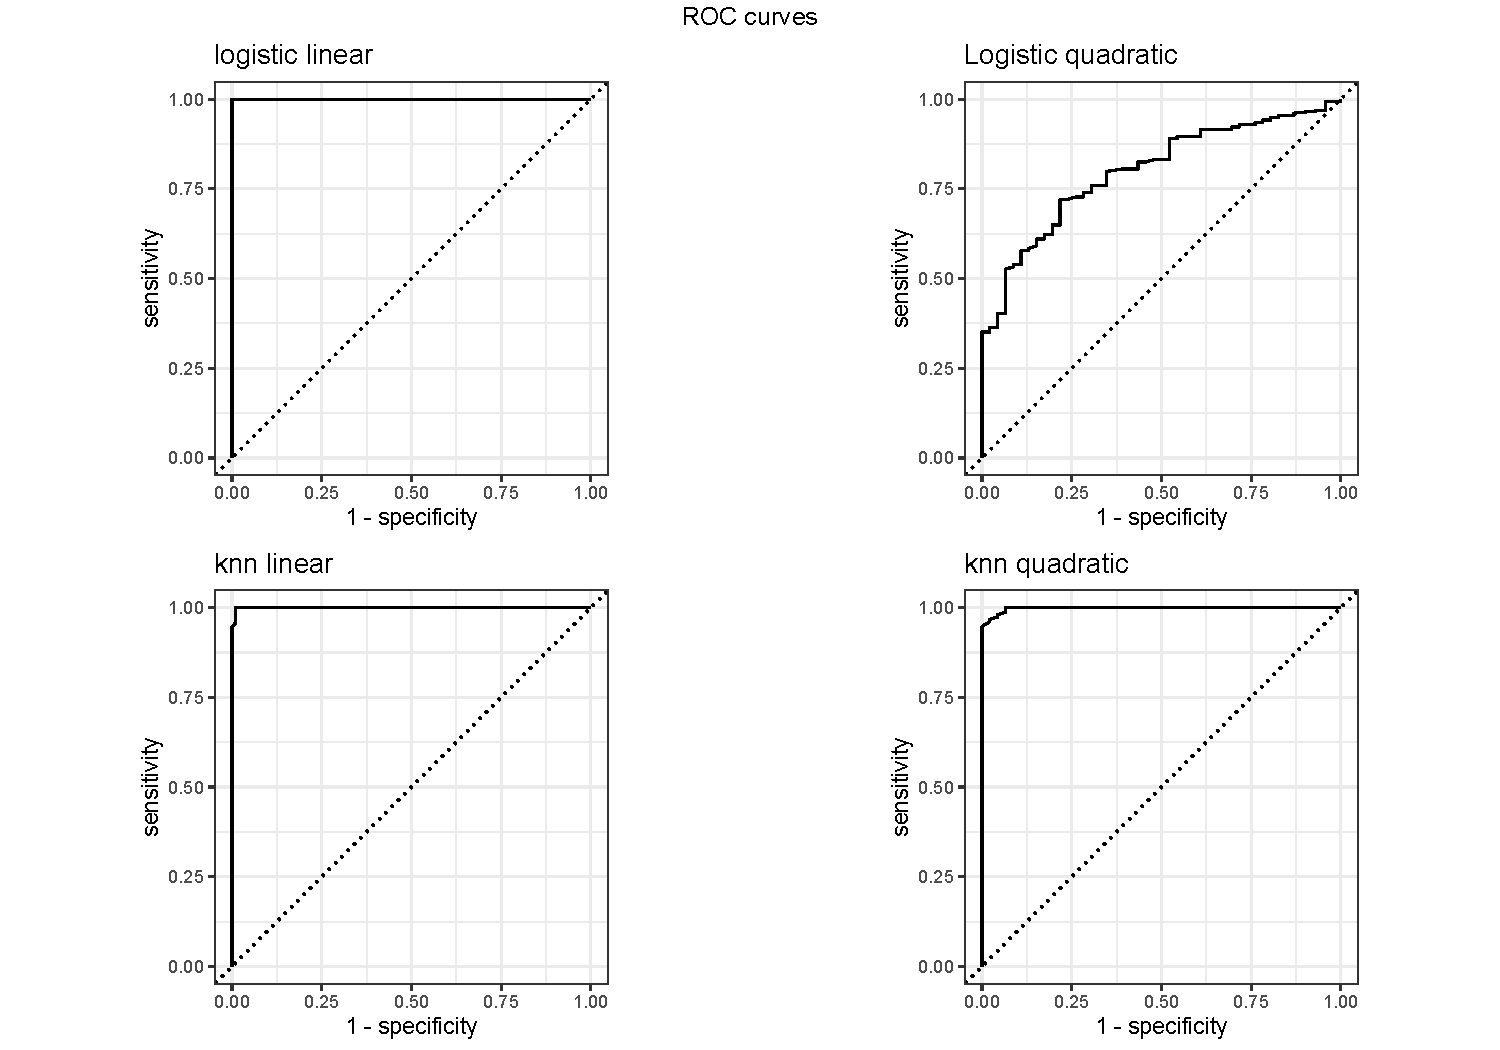
\includegraphics{_main_files/figure-beamer/unnamed-chunk-16-1} \end{center}
\end{block}

\begin{block}{Conclusion}
\protect\hypertarget{conclusion}{}
Given is simplicity and explicit difference between each class, both model perform very well on a dataset with a clear linear bondary. That is visible on both the training and test dataset although with an edge towards the logistic regression.

It is when the boundary aliviates the linearity condition that knn really outshines the logistic output.

It is important to notice that given the fact that the data derive from such strong definitions, it lakes randomness and therefore it's not easy to identify signs of overfitting.
\end{block}
\end{frame}

\begin{frame}[fragile]{Linear Discriminante Analysis vs Decision tree}
\protect\hypertarget{linear-discriminante-analysis-vs-decision-tree}{}
\begin{block}{Dataset definition}
\protect\hypertarget{dataset-definition-1}{}
Lorem ipsum dolor sit amet, consectetur adipiscing elit. Duis eu dictum lorem, et placerat dui. Donec porttitor posuere nisi, non tempor tellus ornare ut. Vestibulum vehicula libero eget consequat lobortis. Suspendisse vel arcu et urna iaculis mattis. Nulla ut mattis est. Pellentesque eu eleifend augue. Maecenas placerat tortor tincidunt risus rutrum tincidunt.

\begin{center}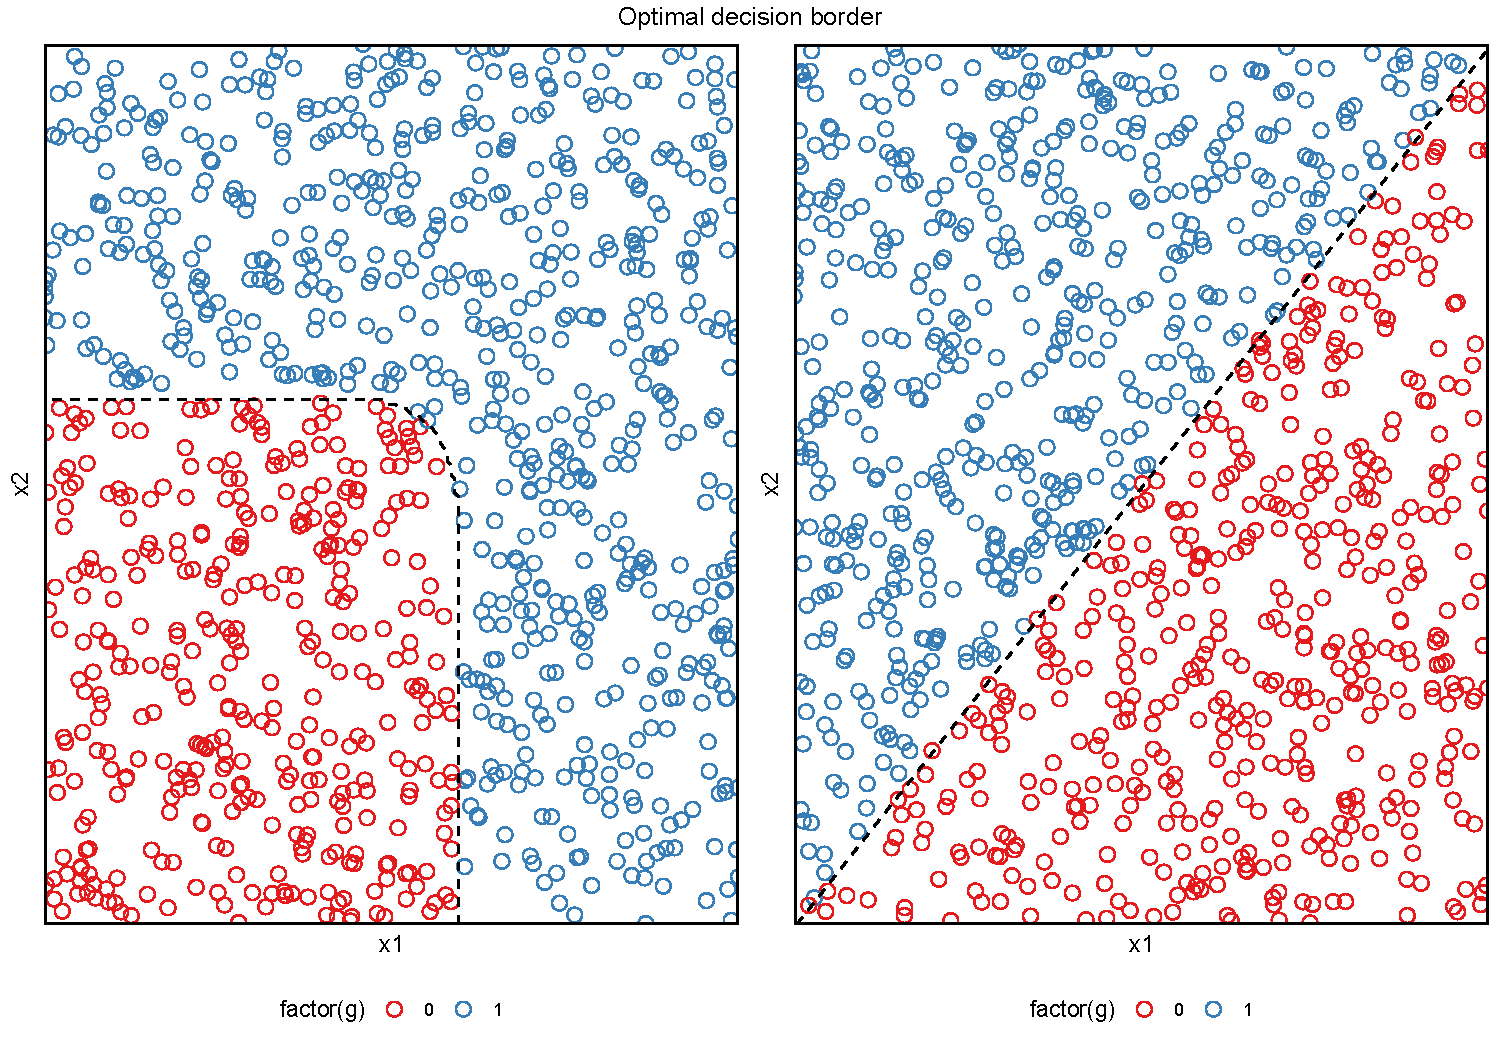
\includegraphics{_main_files/figure-beamer/unnamed-chunk-20-1} \end{center}
\end{block}

\begin{block}{Model fitting}
\protect\hypertarget{model-fitting-1}{}
Lorem ipsum dolor sit amet, consectetur adipiscing elit. Duis eu dictum lorem, et placerat dui. Donec porttitor posuere nisi, non tempor tellus ornare ut. Vestibulum vehicula libero eget consequat lobortis. Suspendisse vel arcu et urna iaculis mattis. Nulla ut mattis est. Pellentesque eu eleifend augue. Maecenas placerat tortor tincidunt risus rutrum tincidunt.

\begin{Shaded}
\begin{Highlighting}[]
\CommentTok{\# 0. Separate test and train}

\NormalTok{data\_lda }\OtherTok{\textless{}{-}}\NormalTok{ dataset\_lda}\SpecialCharTok{$}\NormalTok{dataset}
\NormalTok{data\_lda}\SpecialCharTok{$}\NormalTok{g }\OtherTok{\textless{}{-}} \FunctionTok{factor}\NormalTok{(data\_lda}\SpecialCharTok{$}\NormalTok{g)}

\NormalTok{split }\OtherTok{\textless{}{-}} \FunctionTok{initial\_split}\NormalTok{(data\_lda, }\AttributeTok{prop =} \FloatTok{0.8}\NormalTok{)}

\NormalTok{train\_data\_lda }\OtherTok{\textless{}{-}} \FunctionTok{training}\NormalTok{(split)}
\NormalTok{test\_data\_lda }\OtherTok{\textless{}{-}} \FunctionTok{testing}\NormalTok{(split)}




\NormalTok{data\_dtree }\OtherTok{\textless{}{-}}\NormalTok{ dataset\_dtree}\SpecialCharTok{$}\NormalTok{dataset}
\NormalTok{data\_dtree}\SpecialCharTok{$}\NormalTok{g }\OtherTok{\textless{}{-}} \FunctionTok{factor}\NormalTok{(data\_dtree}\SpecialCharTok{$}\NormalTok{g)}

\NormalTok{split }\OtherTok{\textless{}{-}} \FunctionTok{initial\_split}\NormalTok{(data\_dtree, }\AttributeTok{prop =} \FloatTok{0.8}\NormalTok{)}

\NormalTok{train\_data\_dtree }\OtherTok{\textless{}{-}} \FunctionTok{training}\NormalTok{(split)}
\NormalTok{test\_data\_dtree }\OtherTok{\textless{}{-}} \FunctionTok{testing}\NormalTok{(split)}
\end{Highlighting}
\end{Shaded}

\begin{block}{LDA}
\protect\hypertarget{lda}{}
Lorem ipsum dolor sit amet, consectetur adipiscing elit. Duis eu dictum lorem, et placerat dui. Donec porttitor posuere nisi, non tempor tellus ornare ut. Vestibulum vehicula libero eget consequat lobortis. Suspendisse vel arcu et urna iaculis mattis. Nulla ut mattis est. Pellentesque eu eleifend augue. Maecenas placerat tortor tincidunt risus rutrum tincidunt.

\begin{Shaded}
\begin{Highlighting}[]
\DocumentationTok{\#\# Create workflow}

\DocumentationTok{\#\#\# LDA regression {-}{-}{-}{-}{-}{-}{-}{-}{-}{-}{-}{-}{-}{-}{-}{-}{-}{-}{-}{-}{-}{-}{-}{-}{-}}


\CommentTok{\# 1. specify the model}
\NormalTok{discrim\_linear\_MASS\_spec }\OtherTok{\textless{}{-}}
  \FunctionTok{discrim\_linear}\NormalTok{() }\SpecialCharTok{\%\textgreater{}\%}
  \FunctionTok{set\_mode}\NormalTok{(}\StringTok{"classification"}\NormalTok{) }\SpecialCharTok{\%\textgreater{}\%}
  \FunctionTok{set\_engine}\NormalTok{(}\StringTok{"MASS"}\NormalTok{)}


\CommentTok{\# 2. preprocessing }
\NormalTok{preprocess }\OtherTok{\textless{}{-}} 
  \FunctionTok{recipe}\NormalTok{(g }\SpecialCharTok{\textasciitilde{}}\NormalTok{ x1 }\SpecialCharTok{+}\NormalTok{ x2 , }\AttributeTok{data =}\NormalTok{ train\_data\_lda)}
  
\CommentTok{\# 3, Buildworkflow}
\NormalTok{lda\_wflow }\OtherTok{\textless{}{-}} 
  \FunctionTok{workflow}\NormalTok{() }\SpecialCharTok{\%\textgreater{}\%} 
  \FunctionTok{add\_model}\NormalTok{(discrim\_linear\_MASS\_spec) }\SpecialCharTok{\%\textgreater{}\%} 
  \FunctionTok{add\_recipe}\NormalTok{(preprocess)}

\CommentTok{\# 4. Fit model}
\NormalTok{fit\_control }\OtherTok{\textless{}{-}} \FunctionTok{control\_resamples}\NormalTok{(}\AttributeTok{save\_pred =} \ConstantTok{TRUE}\NormalTok{, }\AttributeTok{save\_workflow =} \ConstantTok{TRUE}\NormalTok{)}

\NormalTok{folds\_lda }\OtherTok{\textless{}{-}} \FunctionTok{vfold\_cv}\NormalTok{(train\_data\_lda, }\AttributeTok{v =} \DecValTok{10}\NormalTok{)}
\NormalTok{folds\_dtree }\OtherTok{\textless{}{-}} \FunctionTok{vfold\_cv}\NormalTok{(train\_data\_dtree, }\AttributeTok{v =} \DecValTok{10}\NormalTok{)}


\NormalTok{lda\_metrics\_dataset\_lda }\OtherTok{\textless{}{-}} 
\NormalTok{  lda\_wflow }\SpecialCharTok{\%\textgreater{}\%} 
  \FunctionTok{fit\_resamples}\NormalTok{(folds\_lda, }\AttributeTok{verbose =} \ConstantTok{TRUE}\NormalTok{, }\AttributeTok{control =}\NormalTok{ fit\_control)}
\end{Highlighting}
\end{Shaded}

\begin{verbatim}
## Warning: The `...` are not used in this function but one or more objects were
## passed: 'verbose'
\end{verbatim}

\begin{Shaded}
\begin{Highlighting}[]
\NormalTok{lda\_metrics\_dataset\_dtree }\OtherTok{\textless{}{-}} 
\NormalTok{  lda\_wflow }\SpecialCharTok{\%\textgreater{}\%} 
  \FunctionTok{fit\_resamples}\NormalTok{(folds\_dtree, }\AttributeTok{verbose =} \ConstantTok{TRUE}\NormalTok{, }\AttributeTok{control =}\NormalTok{ fit\_control)}
\end{Highlighting}
\end{Shaded}

\begin{verbatim}
## Warning: The `...` are not used in this function but one or more objects were
## passed: 'verbose'
\end{verbatim}

\begin{Shaded}
\begin{Highlighting}[]
\CommentTok{\# 5. Performance metrics over the validation set}
\NormalTok{lda\_metrics\_dataset\_lda }\OtherTok{\textless{}{-}} \FunctionTok{collect\_metrics}\NormalTok{(lda\_metrics\_dataset\_lda, }\AttributeTok{summarize =} \ConstantTok{FALSE}\NormalTok{)}
\NormalTok{lda\_metrics\_dataset\_dtree }\OtherTok{\textless{}{-}} \FunctionTok{collect\_metrics}\NormalTok{(lda\_metrics\_dataset\_dtree, }\AttributeTok{summarize =} \ConstantTok{FALSE}\NormalTok{)}


\CommentTok{\# 6. Fits final model}
\NormalTok{lda\_ldaFit }\OtherTok{\textless{}{-}} 
\NormalTok{  lda\_wflow }\SpecialCharTok{\%\textgreater{}\%} 
  \FunctionTok{fit}\NormalTok{(train\_data\_lda)}

\NormalTok{lda\_ldaModel }\OtherTok{\textless{}{-}} \FunctionTok{extract\_fit\_parsnip}\NormalTok{(lda\_ldaFit)}

\NormalTok{lda\_dtreeFit }\OtherTok{\textless{}{-}} 
\NormalTok{  lda\_wflow }\SpecialCharTok{\%\textgreater{}\%} 
  \FunctionTok{fit}\NormalTok{(train\_data\_dtree)}

\NormalTok{lda\_dtreeModel }\OtherTok{\textless{}{-}} \FunctionTok{extract\_fit\_parsnip}\NormalTok{(lda\_dtreeFit)}
\end{Highlighting}
\end{Shaded}
\end{block}
\end{block}

\begin{block}{Decision tree}
\protect\hypertarget{decision-tree}{}
\begin{verbatim}
## Warning: The `...` are not used in this function but one or more objects were passed: 'verbose'
## The `...` are not used in this function but one or more objects were passed: 'verbose'
\end{verbatim}
\end{block}

\begin{block}{Compare results}
\protect\hypertarget{compare-results-1}{}
The plots below show the resulting decision bondaries

\begin{center}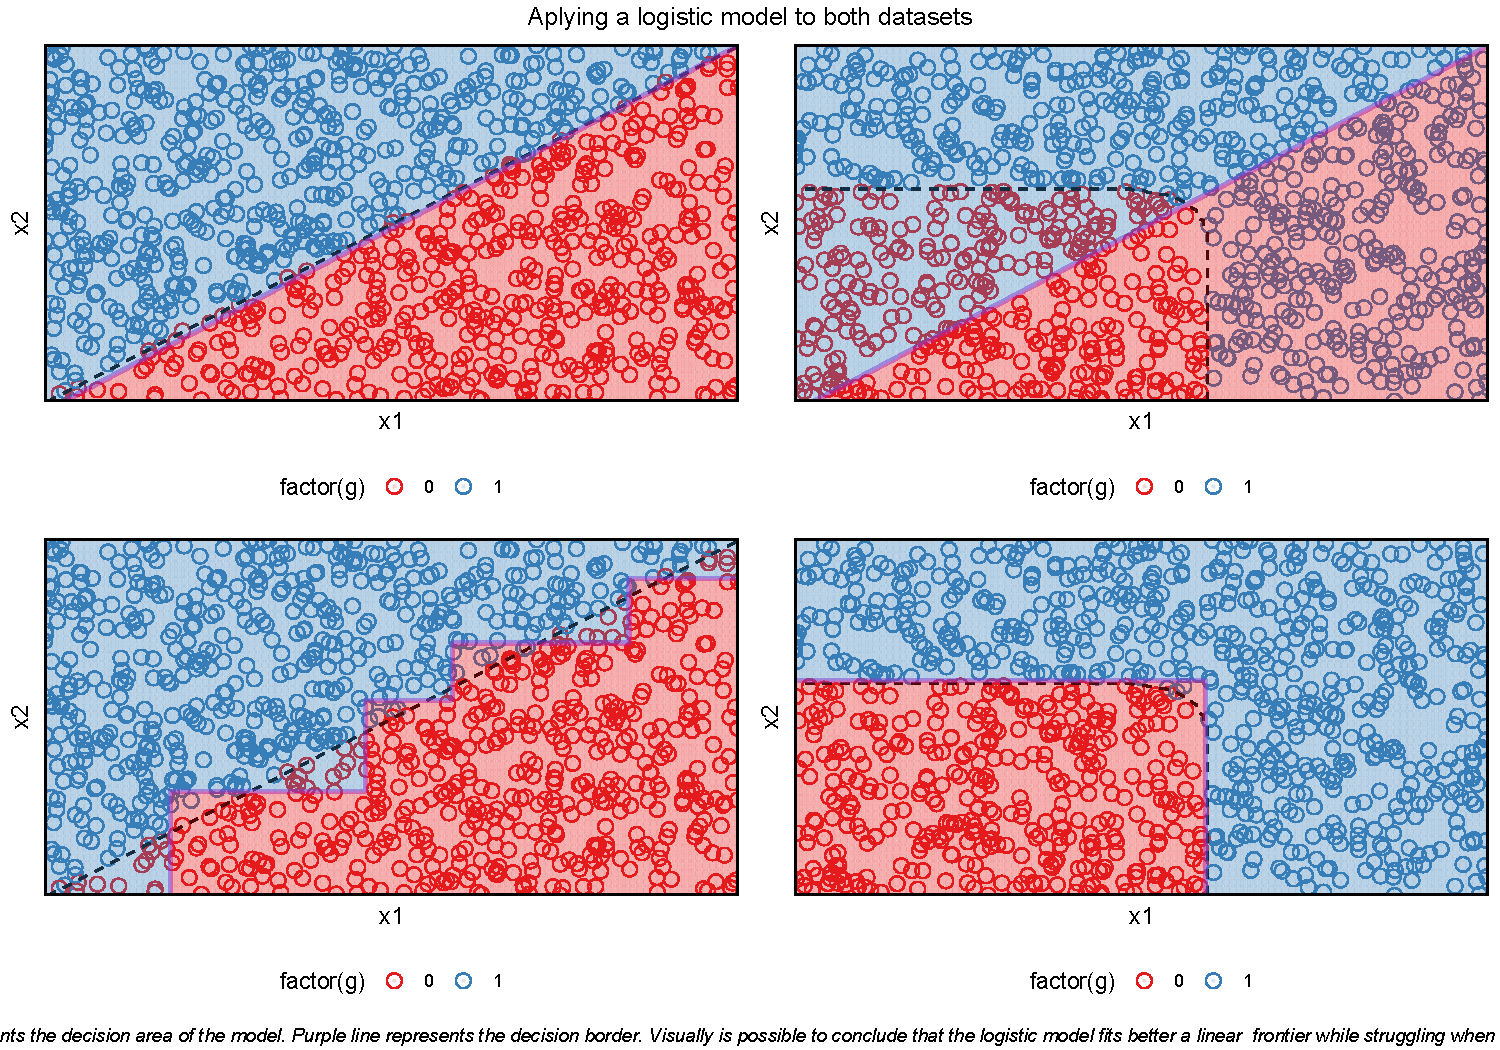
\includegraphics{_main_files/figure-beamer/unnamed-chunk-28-1} \end{center}

The plots shows the evolution of key metrics over crossvalidation trainning

\begin{center}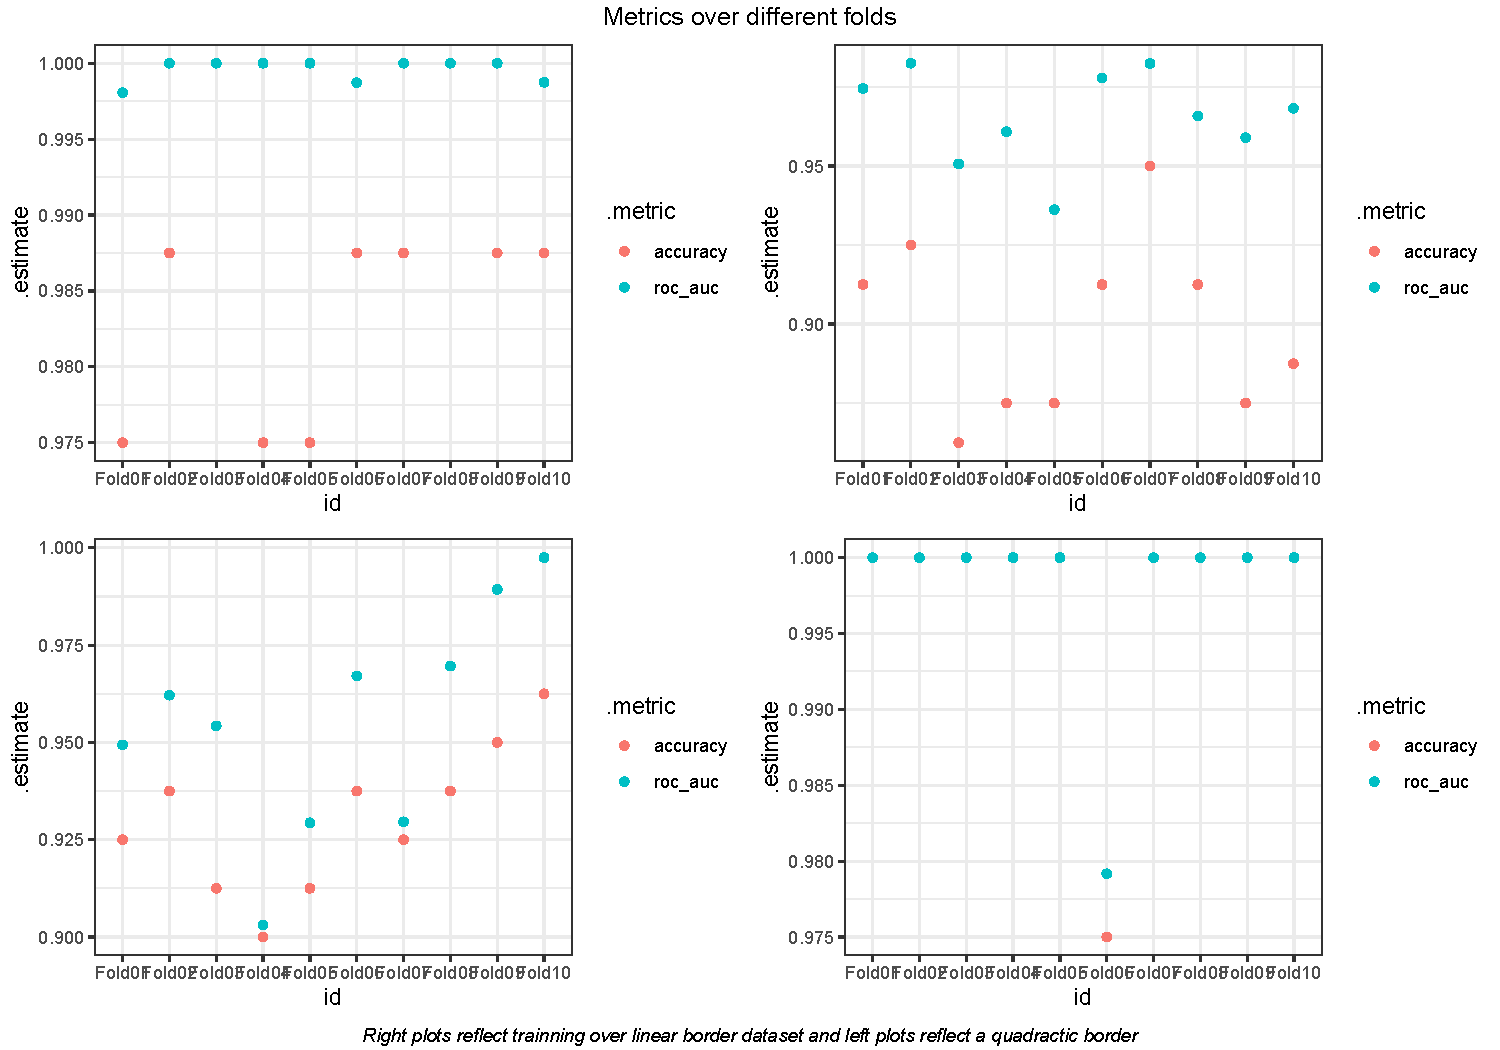
\includegraphics{_main_files/figure-beamer/unnamed-chunk-29-1} \end{center}

The plots show the metrics between different models

\begin{center}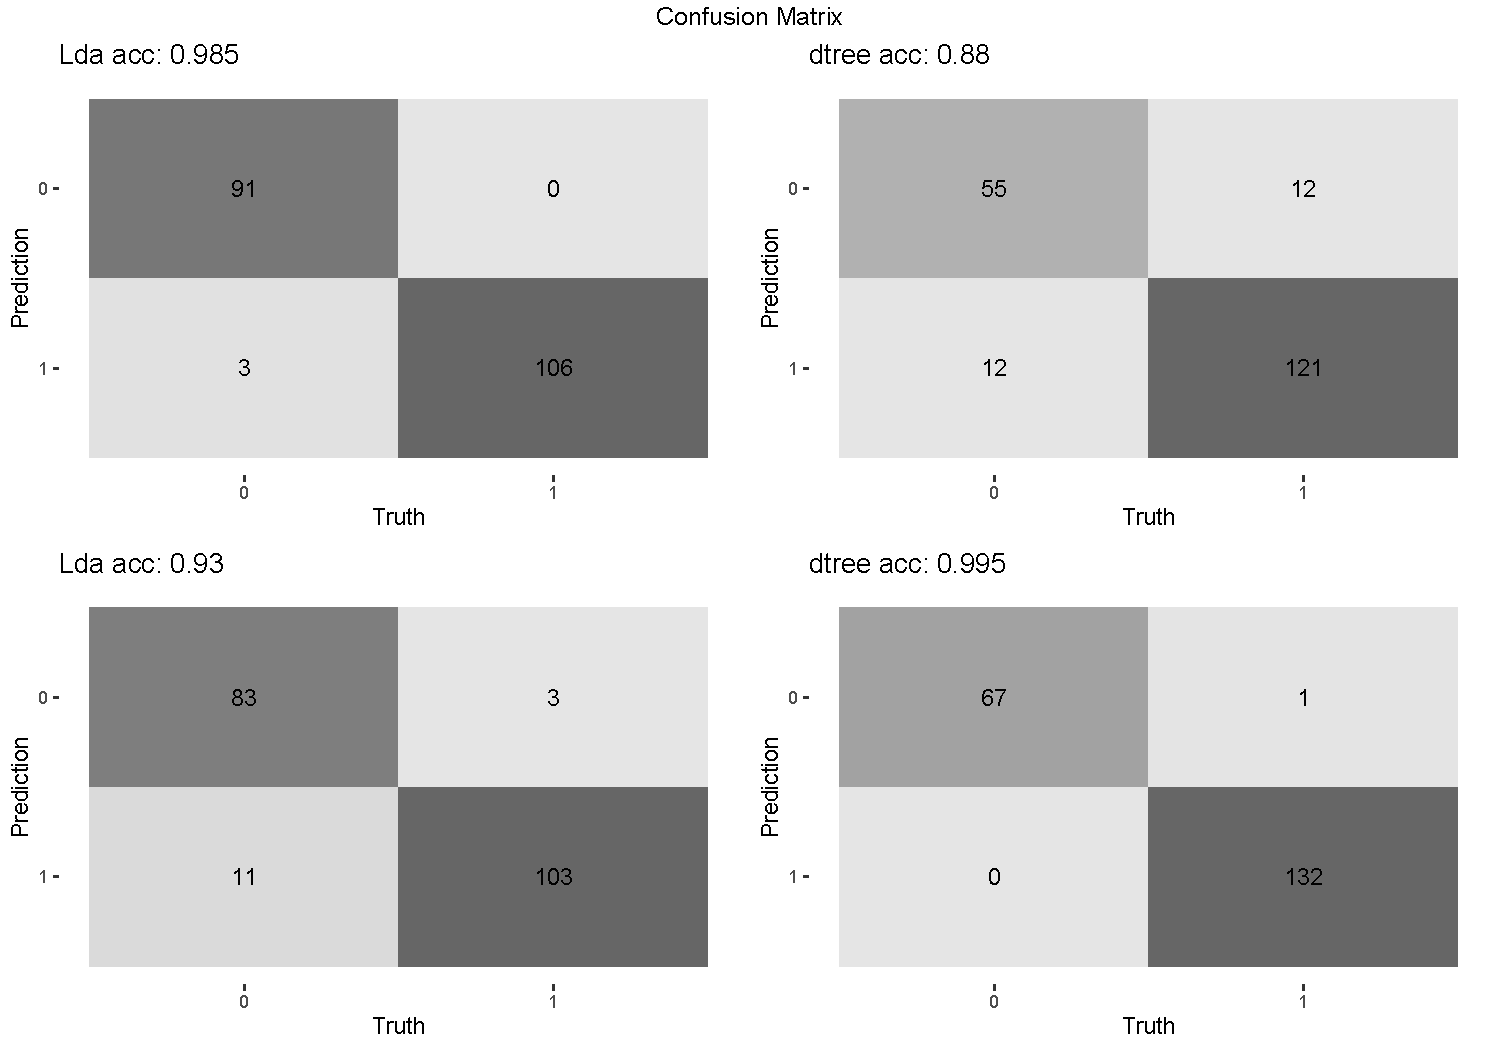
\includegraphics{_main_files/figure-beamer/unnamed-chunk-30-1} \end{center}

\begin{center}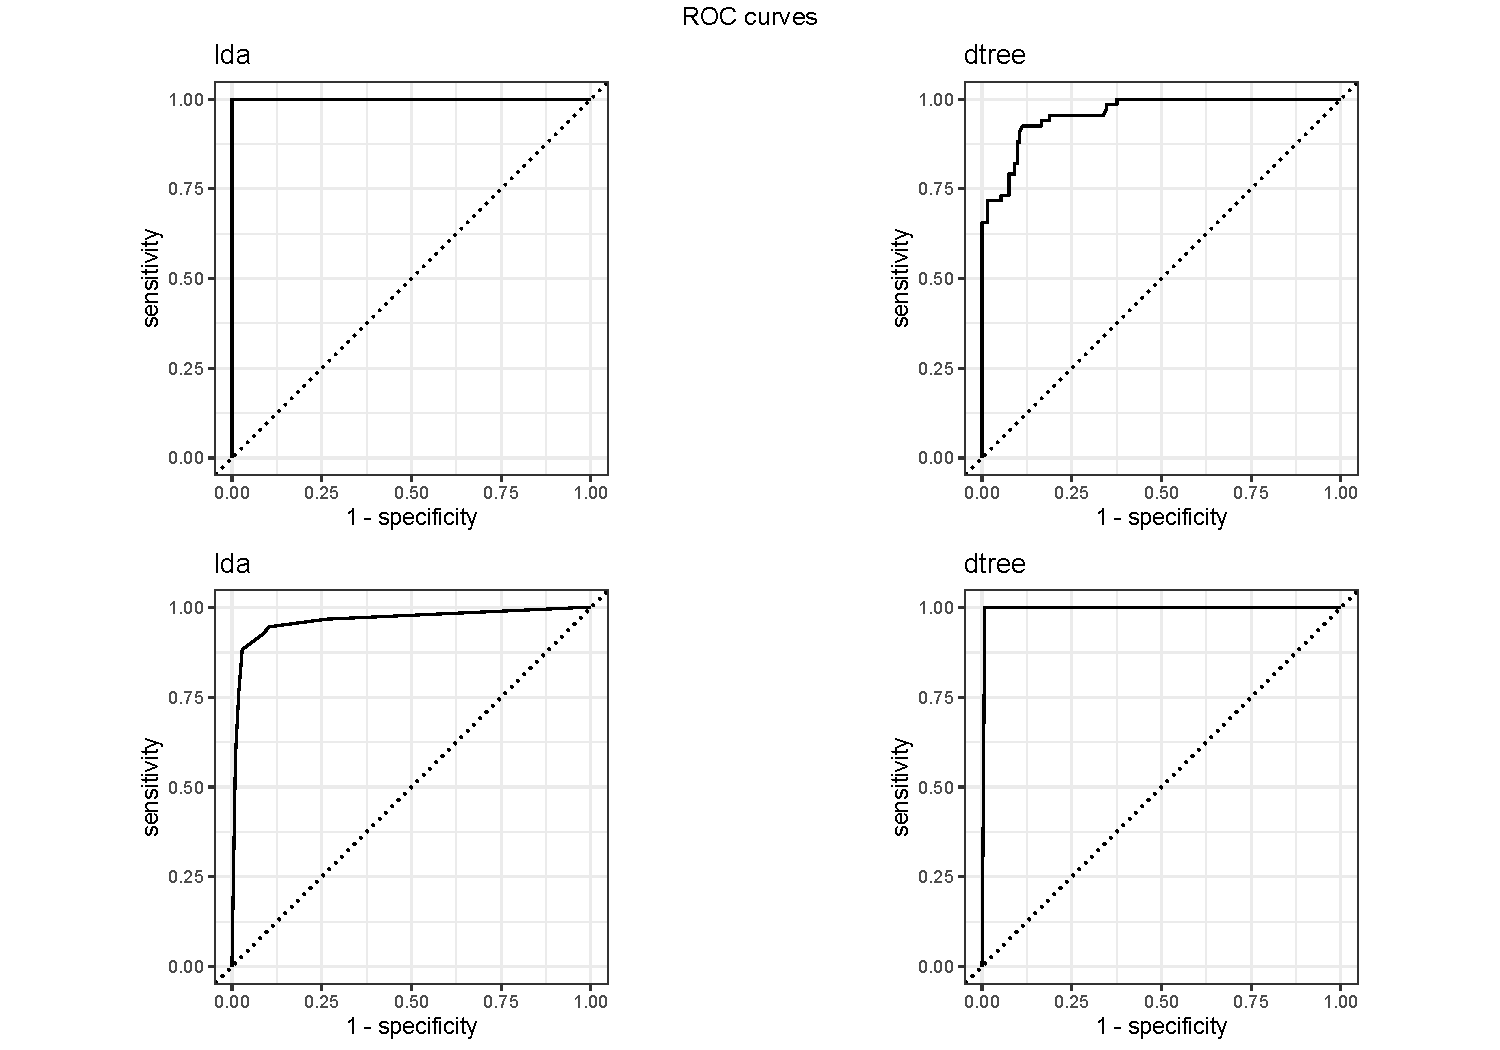
\includegraphics{_main_files/figure-beamer/unnamed-chunk-31-1} \end{center}
\end{block}

\begin{block}{Conclusion}
\protect\hypertarget{conclusion-1}{}
Lorem ipsum dolor sit amet, consectetur adipiscing elit. Duis eu dictum lorem, et placerat dui. Donec porttitor posuere nisi, non tempor tellus ornare ut. Vestibulum vehicula libero eget consequat lobortis. Suspendisse vel arcu et urna iaculis mattis. Nulla ut mattis est. Pellentesque eu eleifend augue. Maecenas placerat tortor tincidunt risus rutrum tincidunt.
\end{block}
\end{frame}

\begin{frame}{Linear Discriminante Analysis vs Decision tree}
\protect\hypertarget{linear-discriminante-analysis-vs-decision-tree-1}{}
\begin{center}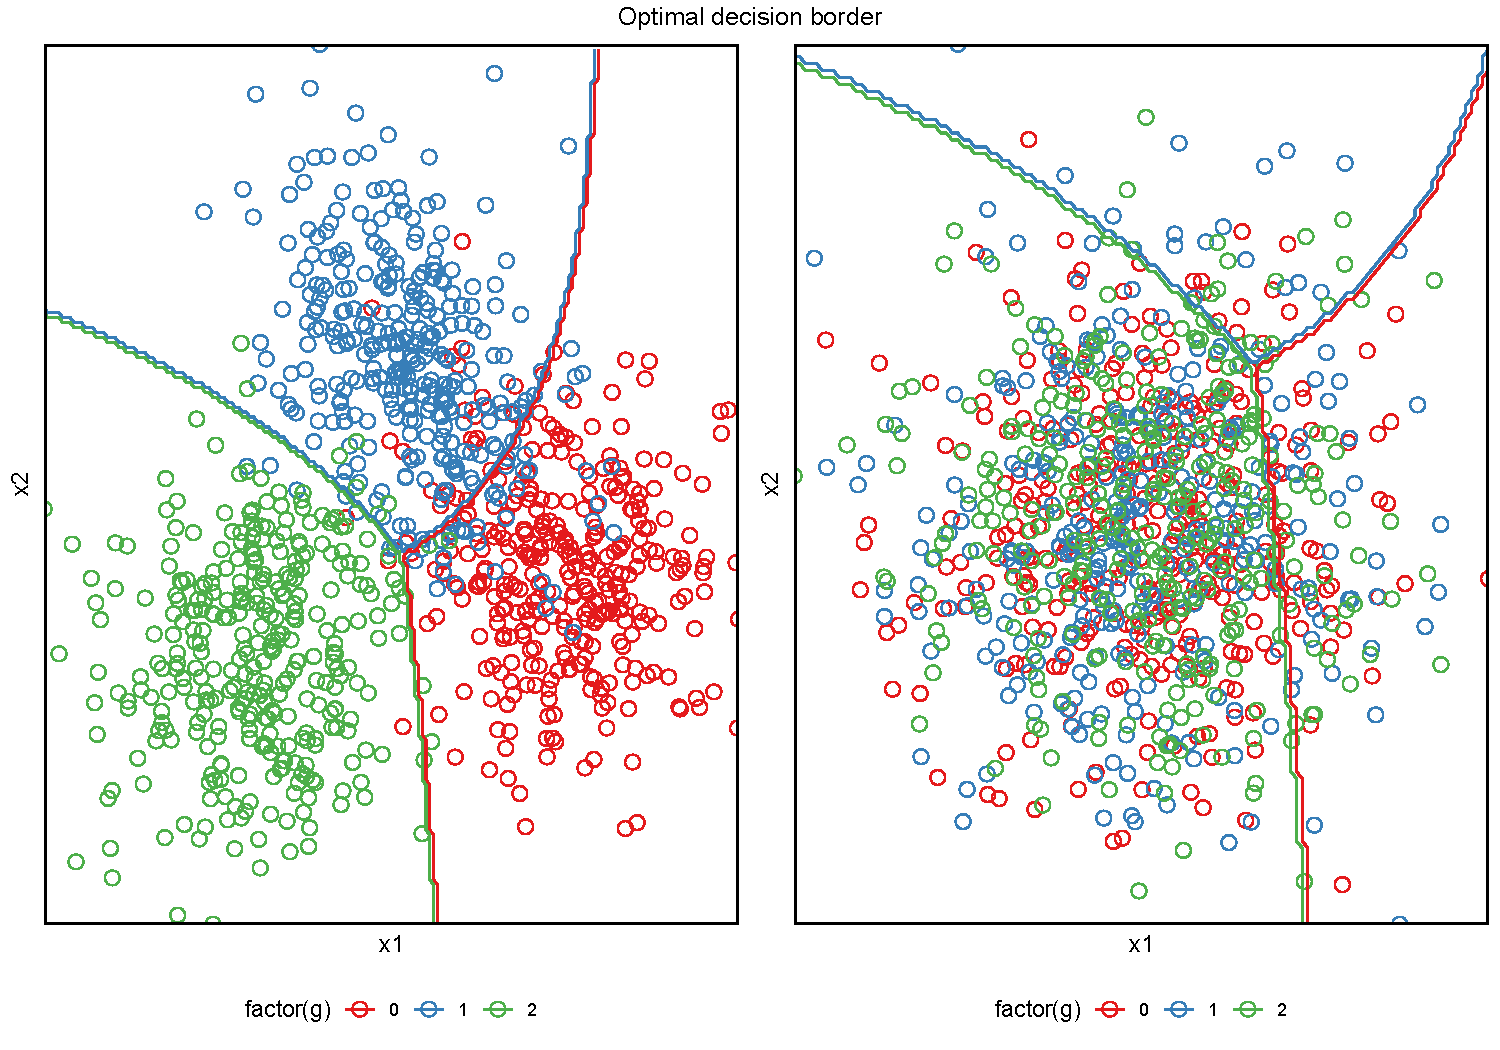
\includegraphics{_main_files/figure-beamer/unnamed-chunk-37-1} \end{center}
\end{frame}

\begin{frame}[fragile]{Linear Discriminante Analysis vs Logistic Regression}
\protect\hypertarget{linear-discriminante-analysis-vs-logistic-regression}{}
\begin{block}{Dataset definition}
\protect\hypertarget{dataset-definition-2}{}
Lorem ipsum dolor sit amet, consectetur adipiscing elit. Duis eu dictum lorem, et placerat dui. Donec porttitor posuere nisi, non tempor tellus ornare ut. Vestibulum vehicula libero eget consequat lobortis. Suspendisse vel arcu et urna iaculis mattis. Nulla ut mattis est. Pellentesque eu eleifend augue. Maecenas placerat tortor tincidunt risus rutrum tincidunt.

\begin{center}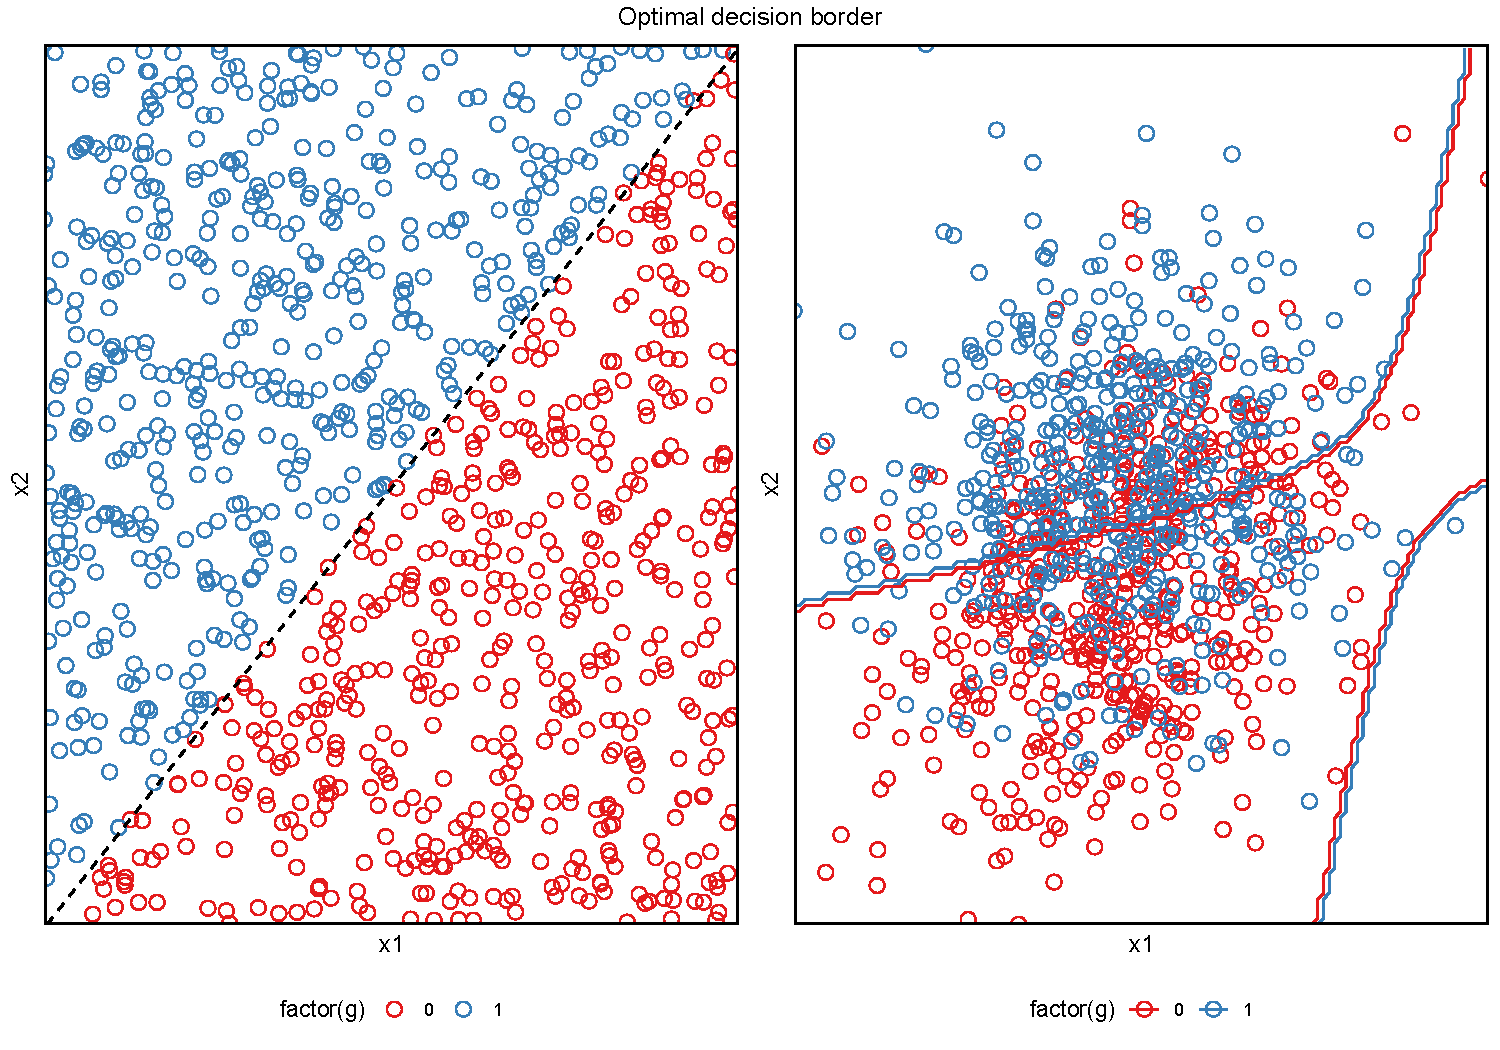
\includegraphics{_main_files/figure-beamer/unnamed-chunk-41-1} \end{center}
\end{block}

\begin{block}{Model fitting}
\protect\hypertarget{model-fitting-2}{}
Lorem ipsum dolor sit amet, consectetur adipiscing elit. Duis eu dictum lorem, et placerat dui. Donec porttitor posuere nisi, non tempor tellus ornare ut. Vestibulum vehicula libero eget consequat lobortis. Suspendisse vel arcu et urna iaculis mattis. Nulla ut mattis est. Pellentesque eu eleifend augue. Maecenas placerat tortor tincidunt risus rutrum tincidunt.

\begin{verbatim}
## Warning: The `...` are not used in this function but one or more objects were
## passed: 'verbose'
\end{verbatim}

\begin{verbatim}
## ! Fold01: preprocessor 1/1, model 1/1: glm.fit: algorithm did not converge, glm.fi...
\end{verbatim}

\begin{verbatim}
## ! Fold02: preprocessor 1/1, model 1/1: glm.fit: algorithm did not converge, glm.fi...
\end{verbatim}

\begin{verbatim}
## ! Fold03: preprocessor 1/1, model 1/1: glm.fit: algorithm did not converge, glm.fi...
\end{verbatim}

\begin{verbatim}
## ! Fold04: preprocessor 1/1, model 1/1: glm.fit: algorithm did not converge, glm.fi...
\end{verbatim}

\begin{verbatim}
## ! Fold05: preprocessor 1/1, model 1/1: glm.fit: algorithm did not converge, glm.fi...
\end{verbatim}

\begin{verbatim}
## ! Fold06: preprocessor 1/1, model 1/1: glm.fit: algorithm did not converge, glm.fi...
\end{verbatim}

\begin{verbatim}
## ! Fold07: preprocessor 1/1, model 1/1: glm.fit: algorithm did not converge, glm.fi...
\end{verbatim}

\begin{verbatim}
## ! Fold08: preprocessor 1/1, model 1/1: glm.fit: algorithm did not converge, glm.fi...
\end{verbatim}

\begin{verbatim}
## ! Fold09: preprocessor 1/1, model 1/1: glm.fit: algorithm did not converge, glm.fi...
\end{verbatim}

\begin{verbatim}
## ! Fold10: preprocessor 1/1, model 1/1: glm.fit: algorithm did not converge, glm.fi...
\end{verbatim}

\begin{verbatim}
## Warning: The `...` are not used in this function but one or more objects were
## passed: 'verbose'
\end{verbatim}

\begin{verbatim}
## Warning: glm.fit: algorithm did not converge
\end{verbatim}

\begin{verbatim}
## Warning: glm.fit: fitted probabilities numerically 0 or 1 occurred
\end{verbatim}

\begin{verbatim}
## Warning: The `...` are not used in this function but one or more objects were passed: 'verbose'
## The `...` are not used in this function but one or more objects were passed: 'verbose'
\end{verbatim}
\end{block}

\begin{block}{Compare results}
\protect\hypertarget{compare-results-2}{}
The plots below show the resulting decision boundaries

\begin{center}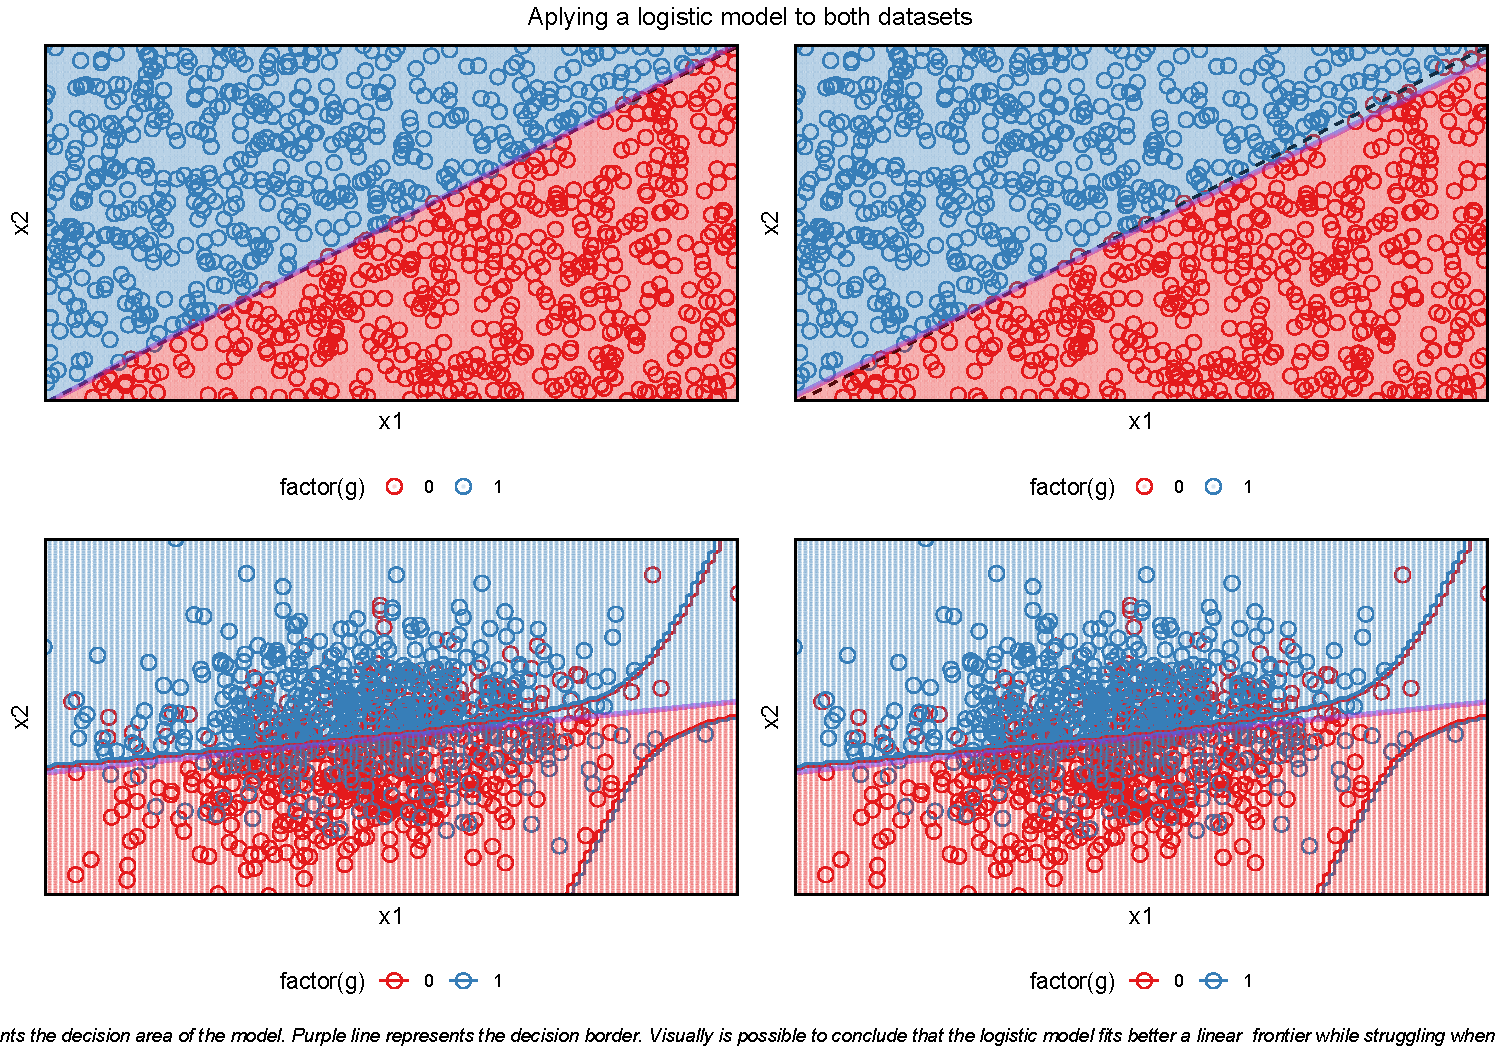
\includegraphics{_main_files/figure-beamer/unnamed-chunk-46-1} \end{center}

The plots shows the evolution of key metrics over crossvalidation trainning

\begin{center}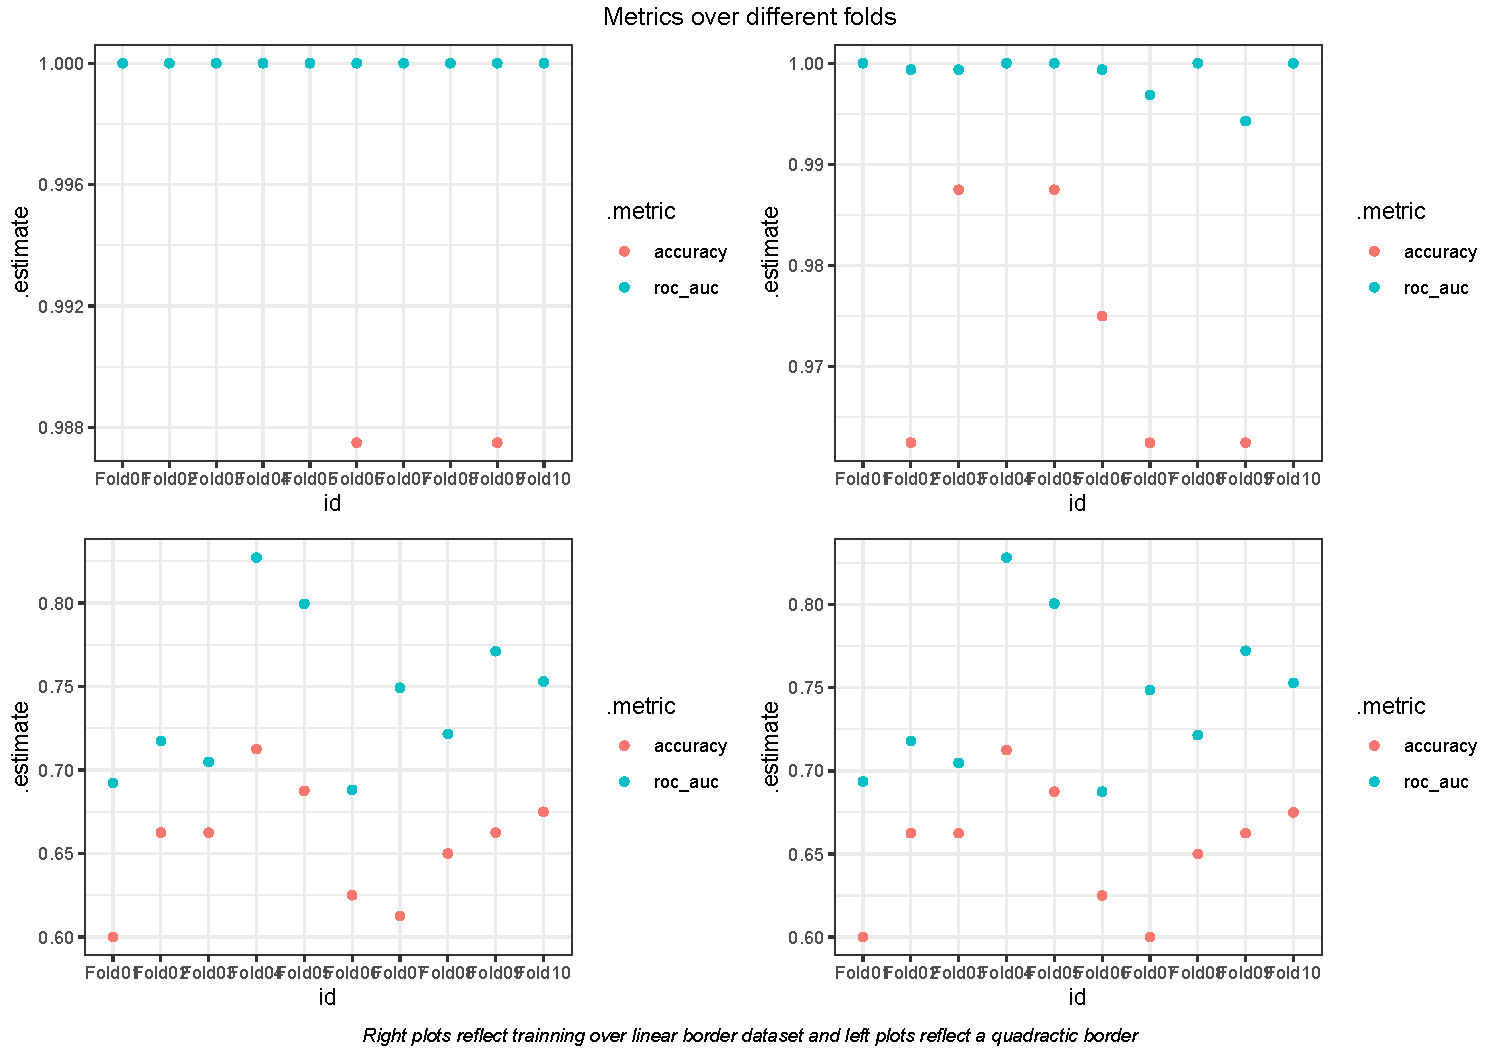
\includegraphics{_main_files/figure-beamer/unnamed-chunk-47-1} \end{center}

The plots show the metrics between different models

\begin{center}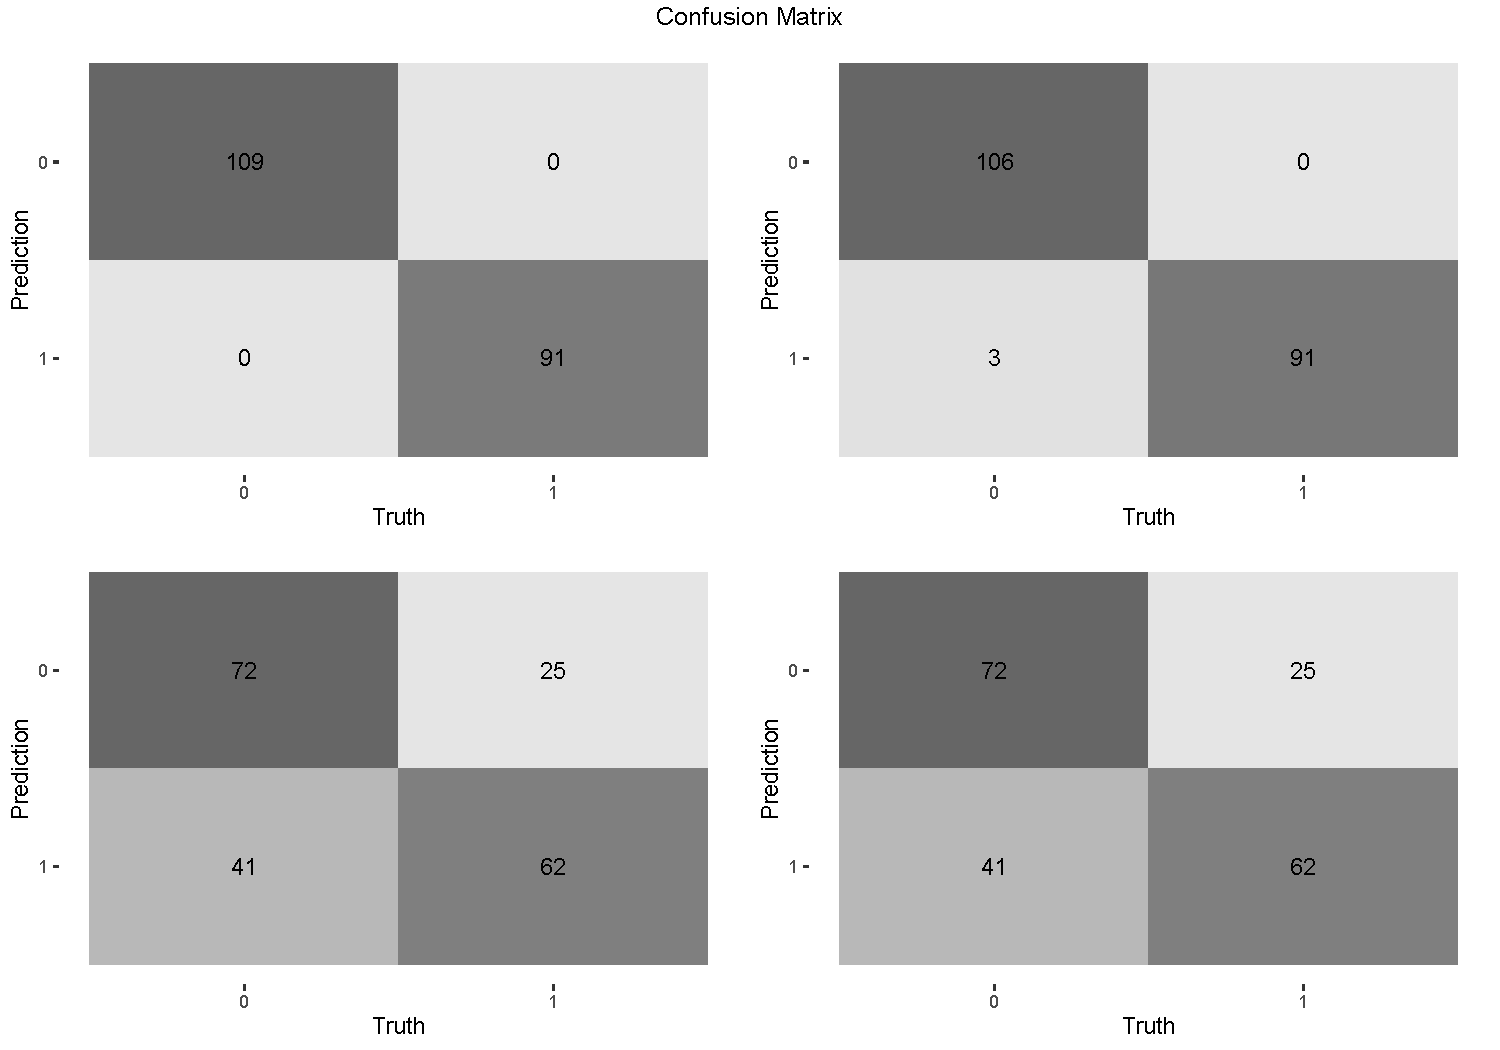
\includegraphics{_main_files/figure-beamer/unnamed-chunk-48-1} \end{center}

\begin{center}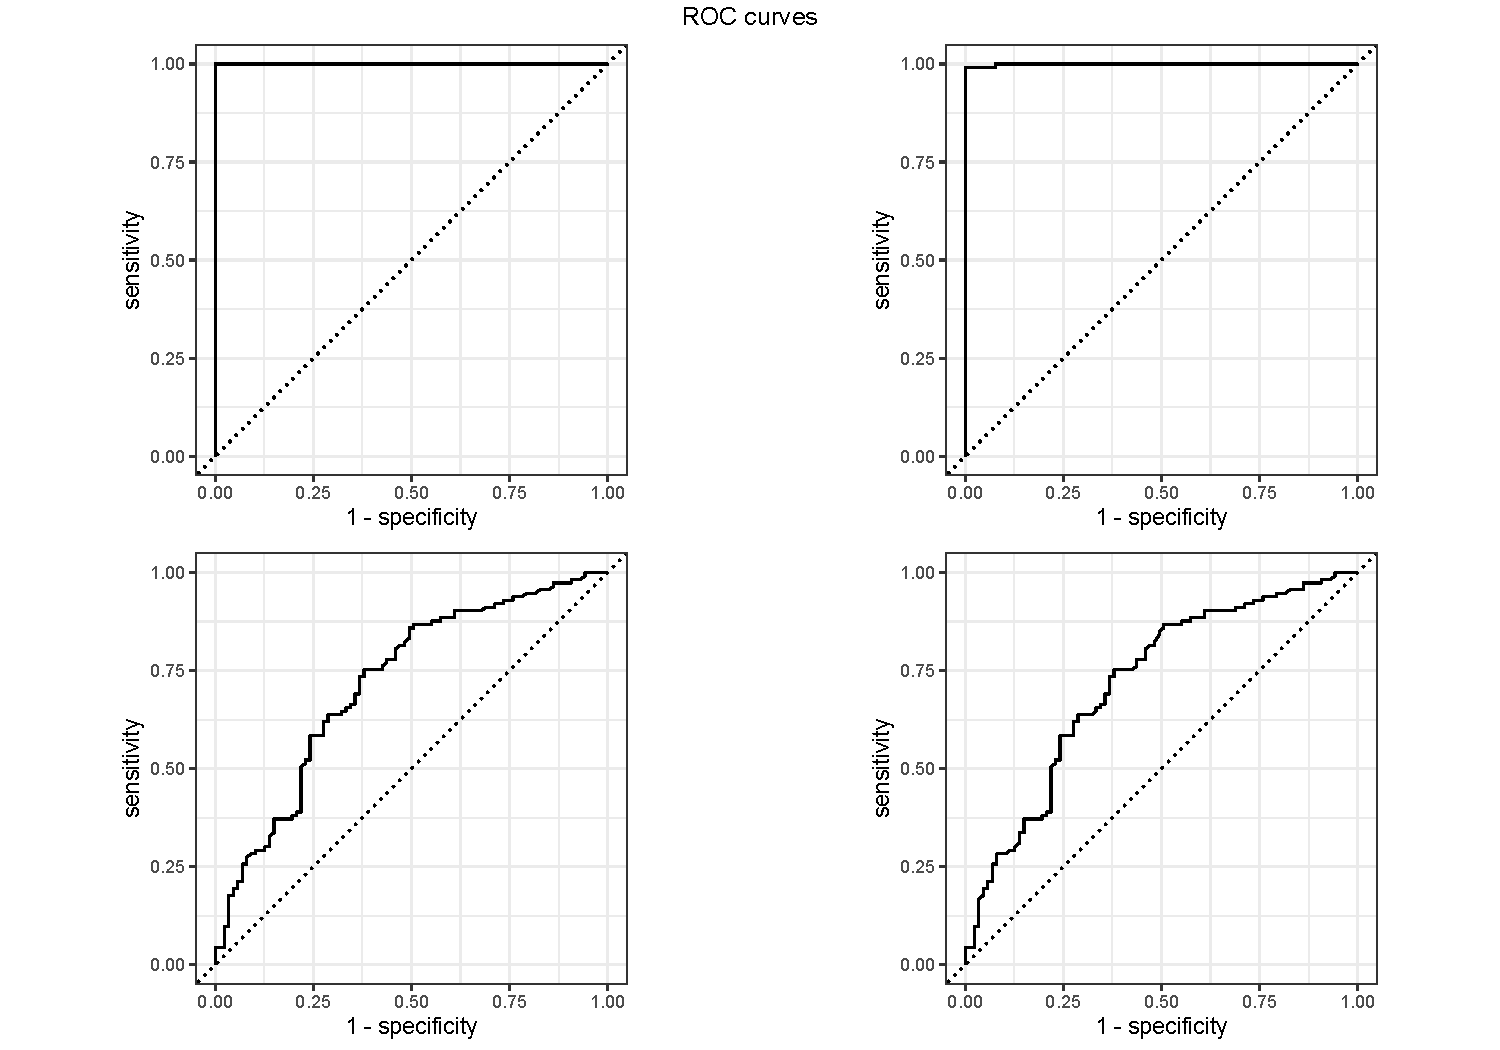
\includegraphics{_main_files/figure-beamer/unnamed-chunk-49-1} \end{center}
\end{block}

\begin{block}{Conclusion}
\protect\hypertarget{conclusion-2}{}
Lorem ipsum dolor sit amet, consectetur adipiscing elit. Duis eu dictum lorem, et placerat dui. Donec porttitor posuere nisi, non tempor tellus ornare ut. Vestibulum vehicula libero eget consequat lobortis. Suspendisse vel arcu et urna iaculis mattis. Nulla ut mattis est. Pellentesque eu eleifend augue. Maecenas placerat tortor tincidunt risus rutrum tincidunt.
\end{block}
\end{frame}

\begin{frame}[fragile]{Decision tree vs tree boosting}
\protect\hypertarget{decision-tree-vs-tree-boosting}{}
\begin{block}{Dataset definition}
\protect\hypertarget{dataset-definition-3}{}
Lorem ipsum dolor sit amet, consectetur adipiscing elit. Duis eu dictum lorem, et placerat dui. Donec porttitor posuere nisi, non tempor tellus ornare ut. Vestibulum vehicula libero eget consequat lobortis. Suspendisse vel arcu et urna iaculis mattis. Nulla ut mattis est. Pellentesque eu eleifend augue. Maecenas placerat tortor tincidunt risus rutrum tincidunt.

\begin{center}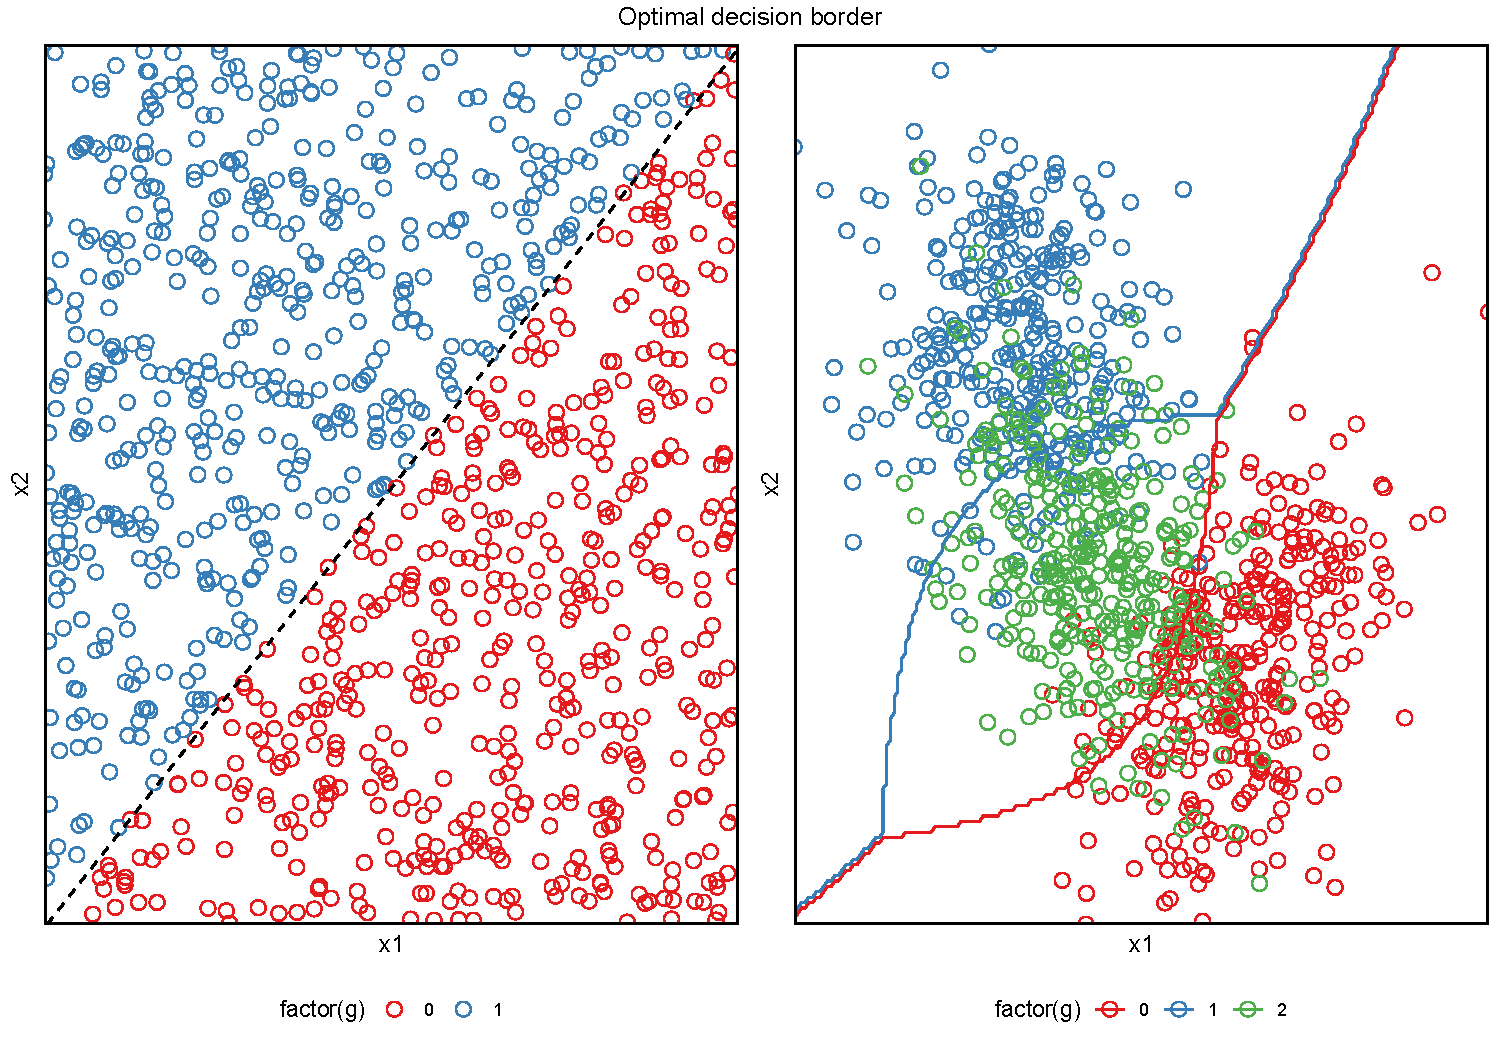
\includegraphics{_main_files/figure-beamer/unnamed-chunk-53-1} \end{center}
\end{block}

\begin{block}{Model fitting}
\protect\hypertarget{model-fitting-3}{}
Lorem ipsum dolor sit amet, consectetur adipiscing elit. Duis eu dictum lorem, et placerat dui. Donec porttitor posuere nisi, non tempor tellus ornare ut. Vestibulum vehicula libero eget consequat lobortis. Suspendisse vel arcu et urna iaculis mattis. Nulla ut mattis est. Pellentesque eu eleifend augue. Maecenas placerat tortor tincidunt risus rutrum tincidunt.

\begin{verbatim}
## Warning: The `...` are not used in this function but one or more objects were passed: 'verbose'
## The `...` are not used in this function but one or more objects were passed: 'verbose'
## The `...` are not used in this function but one or more objects were passed: 'verbose'
## The `...` are not used in this function but one or more objects were passed: 'verbose'
\end{verbatim}
\end{block}

\begin{block}{Compare results}
\protect\hypertarget{compare-results-3}{}
The plots below show the resulting decision boundaries

\begin{center}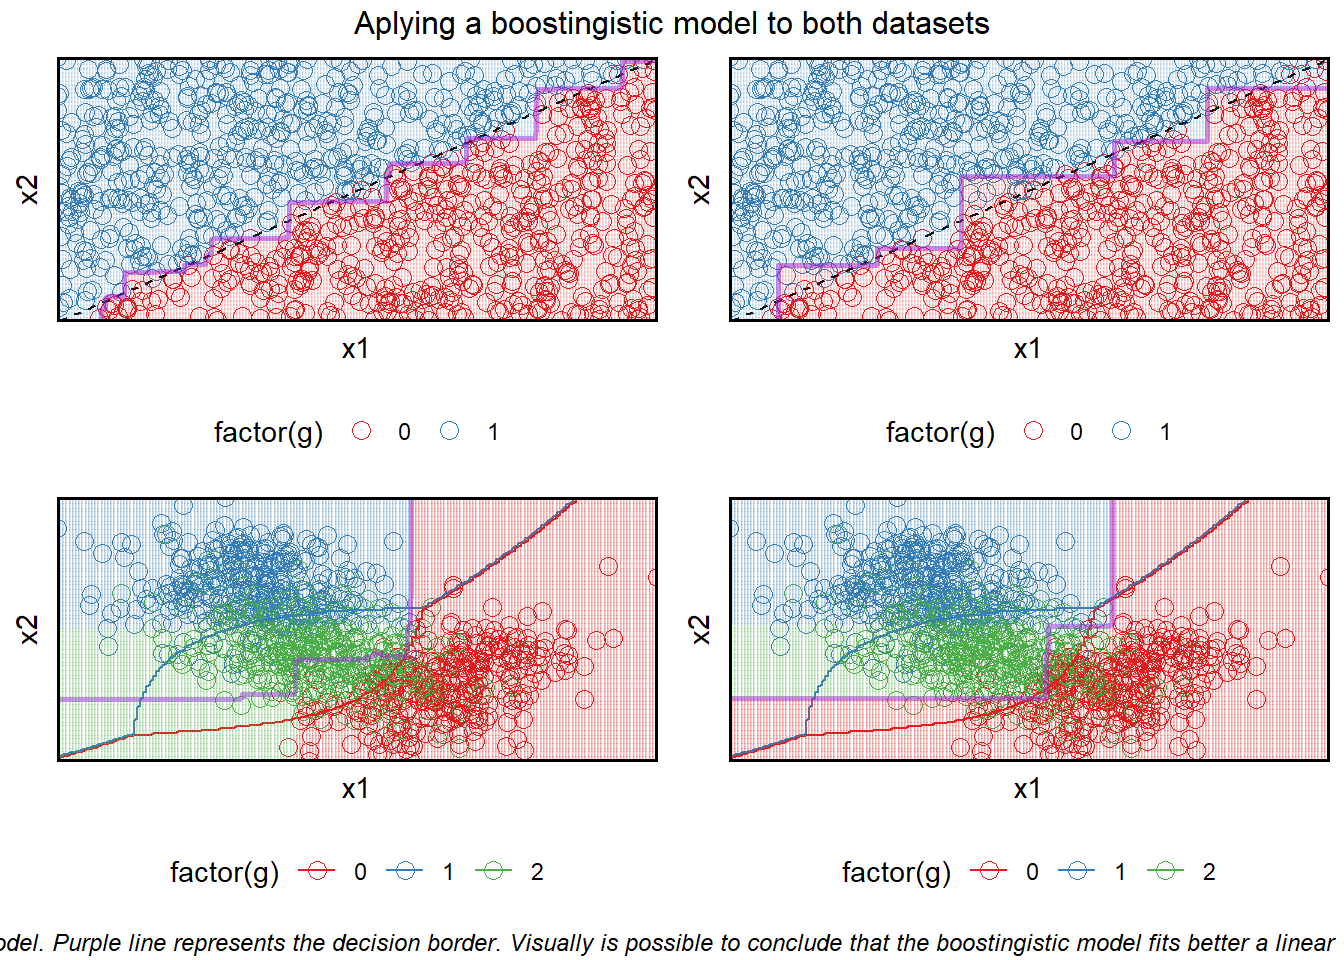
\includegraphics{_main_files/figure-beamer/unnamed-chunk-58-1} \end{center}

The plots shows the evolution of key metrics over crossvalidation trainning

\begin{center}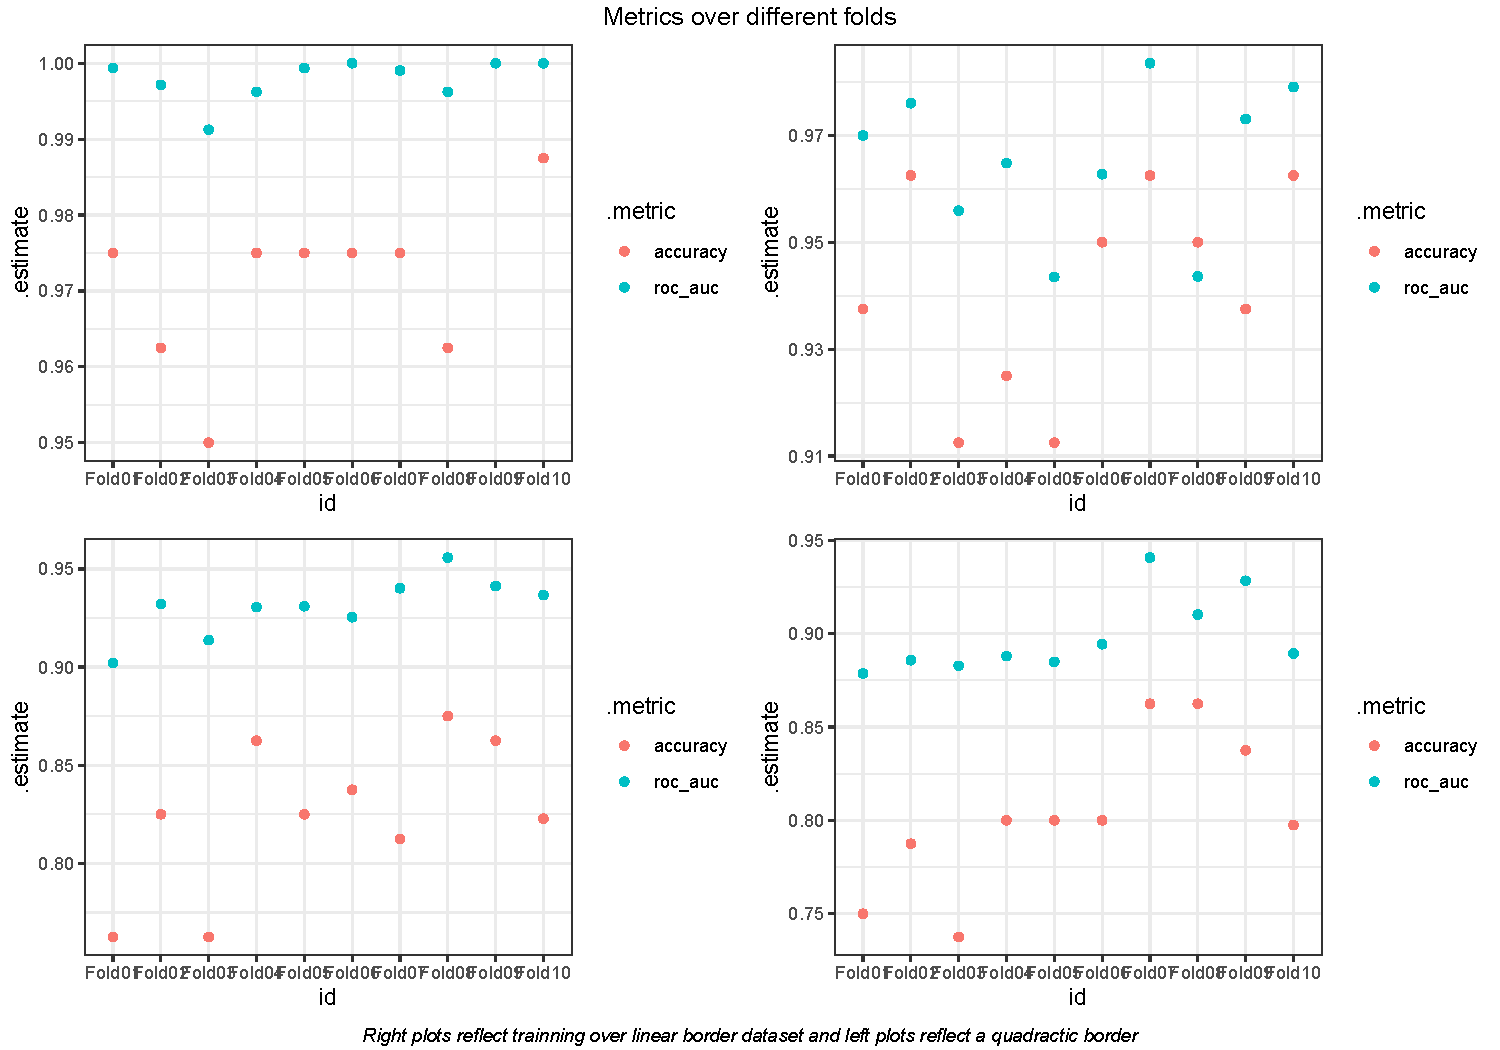
\includegraphics{_main_files/figure-beamer/unnamed-chunk-59-1} \end{center}

The plots show the metrics between different models

\begin{center}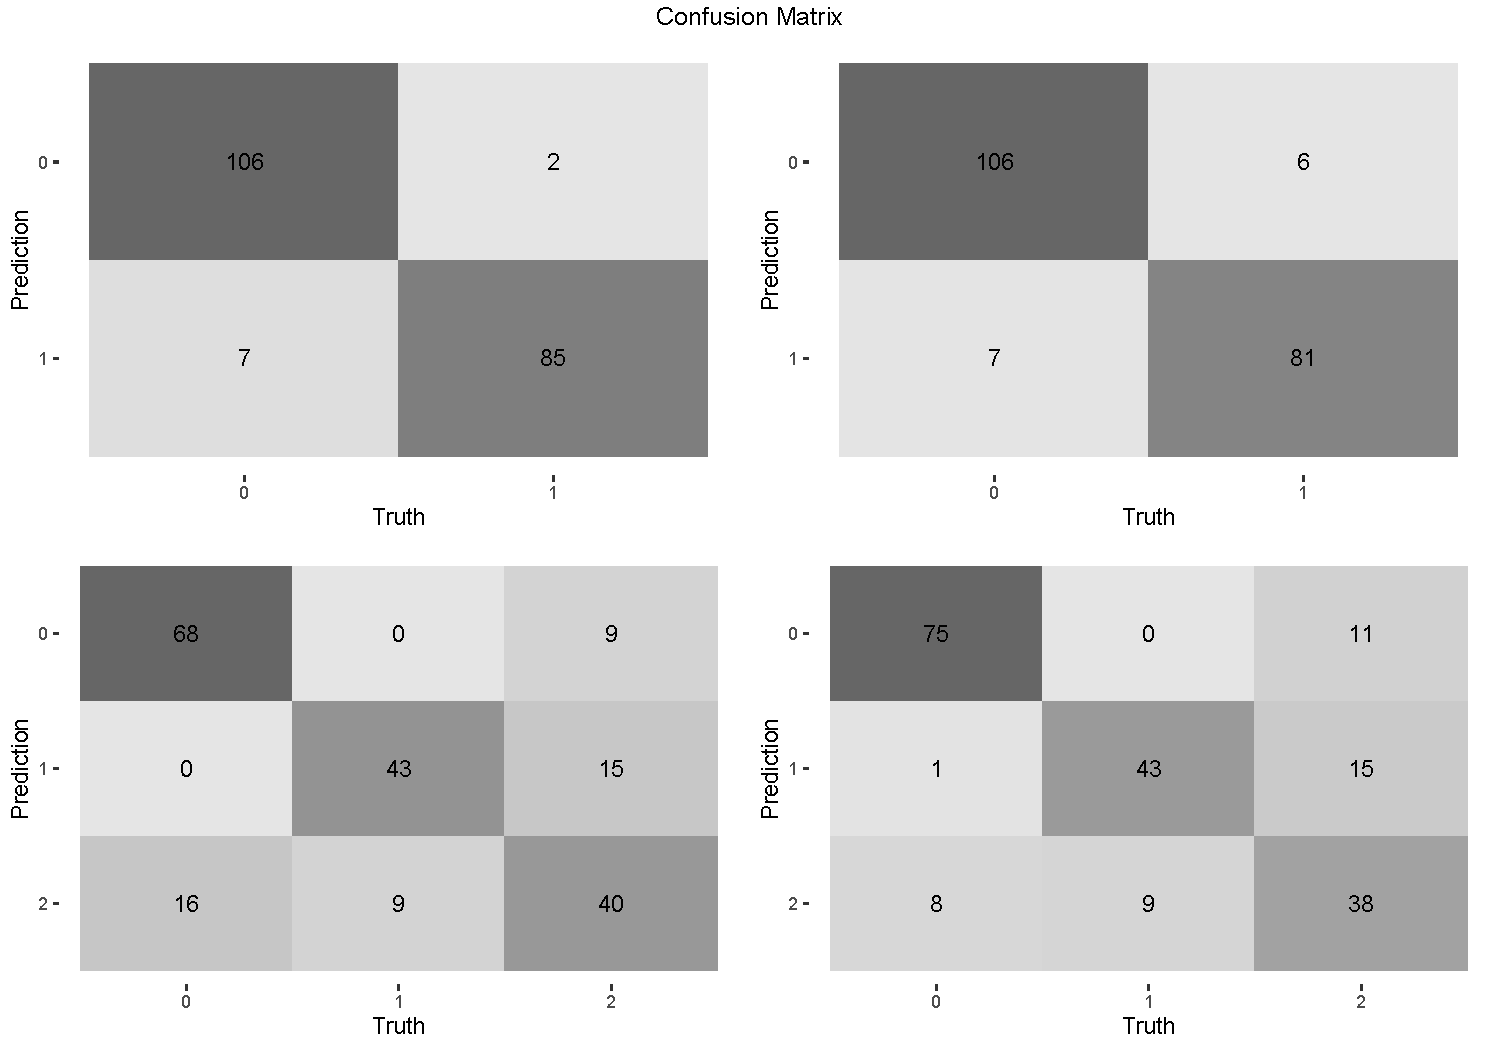
\includegraphics{_main_files/figure-beamer/unnamed-chunk-60-1} \end{center}

\begin{center}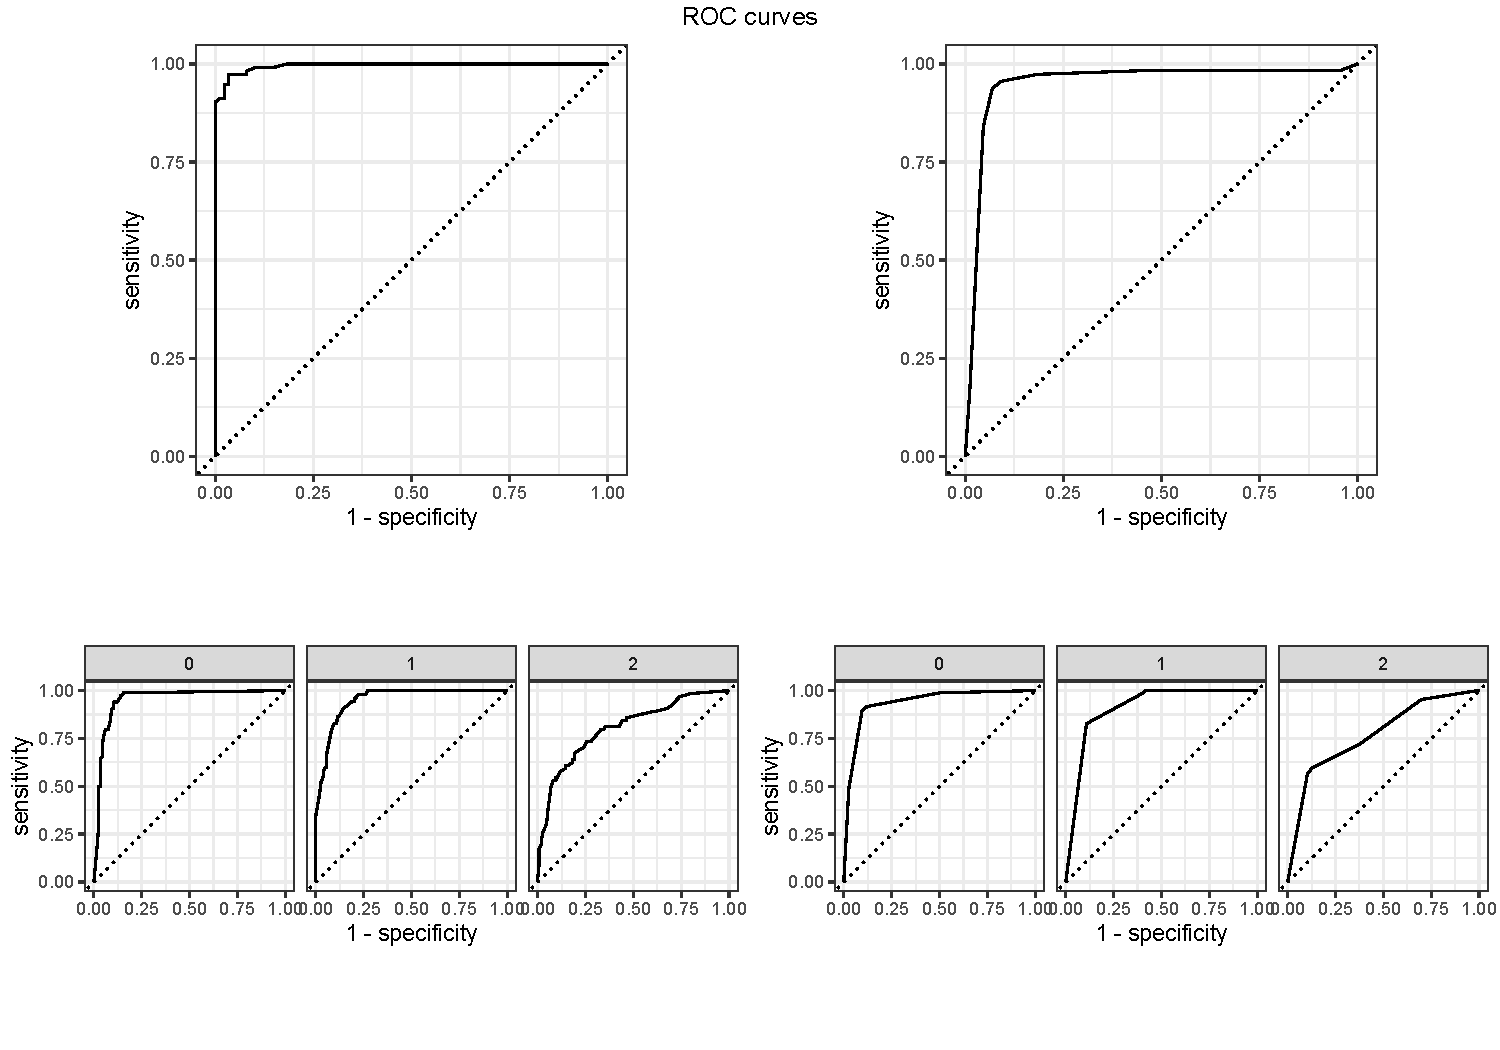
\includegraphics{_main_files/figure-beamer/unnamed-chunk-61-1} \end{center}
\end{block}

\begin{block}{Conclusion}
\protect\hypertarget{conclusion-3}{}
Lorem ipsum dolor sit amet, consectetur adipiscing elit. Duis eu dictum lorem, et placerat dui. Donec porttitor posuere nisi, non tempor tellus ornare ut. Vestibulum vehicula libero eget consequat lobortis. Suspendisse vel arcu et urna iaculis mattis. Nulla ut mattis est. Pellentesque eu eleifend augue. Maecenas placerat tortor tincidunt risus rutrum tincidunt.
\end{block}
\end{frame}

\begin{frame}[fragile]{SVM Radial vs SVM linear}
\protect\hypertarget{svm-radial-vs-svm-linear}{}
\begin{block}{Dataset definition}
\protect\hypertarget{dataset-definition-4}{}
Lorem ipsum dolor sit amet, consectetur adipiscing elit. Duis eu dictum lorem, et placerat dui. Donec porttitor posuere nisi, non tempor tellus ornare ut. Vestibulum vehicula libero eget consequat lobortis. Suspendisse vel arcu et urna iaculis mattis. Nulla ut mattis est. Pellentesque eu eleifend augue. Maecenas placerat tortor tincidunt risus rutrum tincidunt.

\begin{center}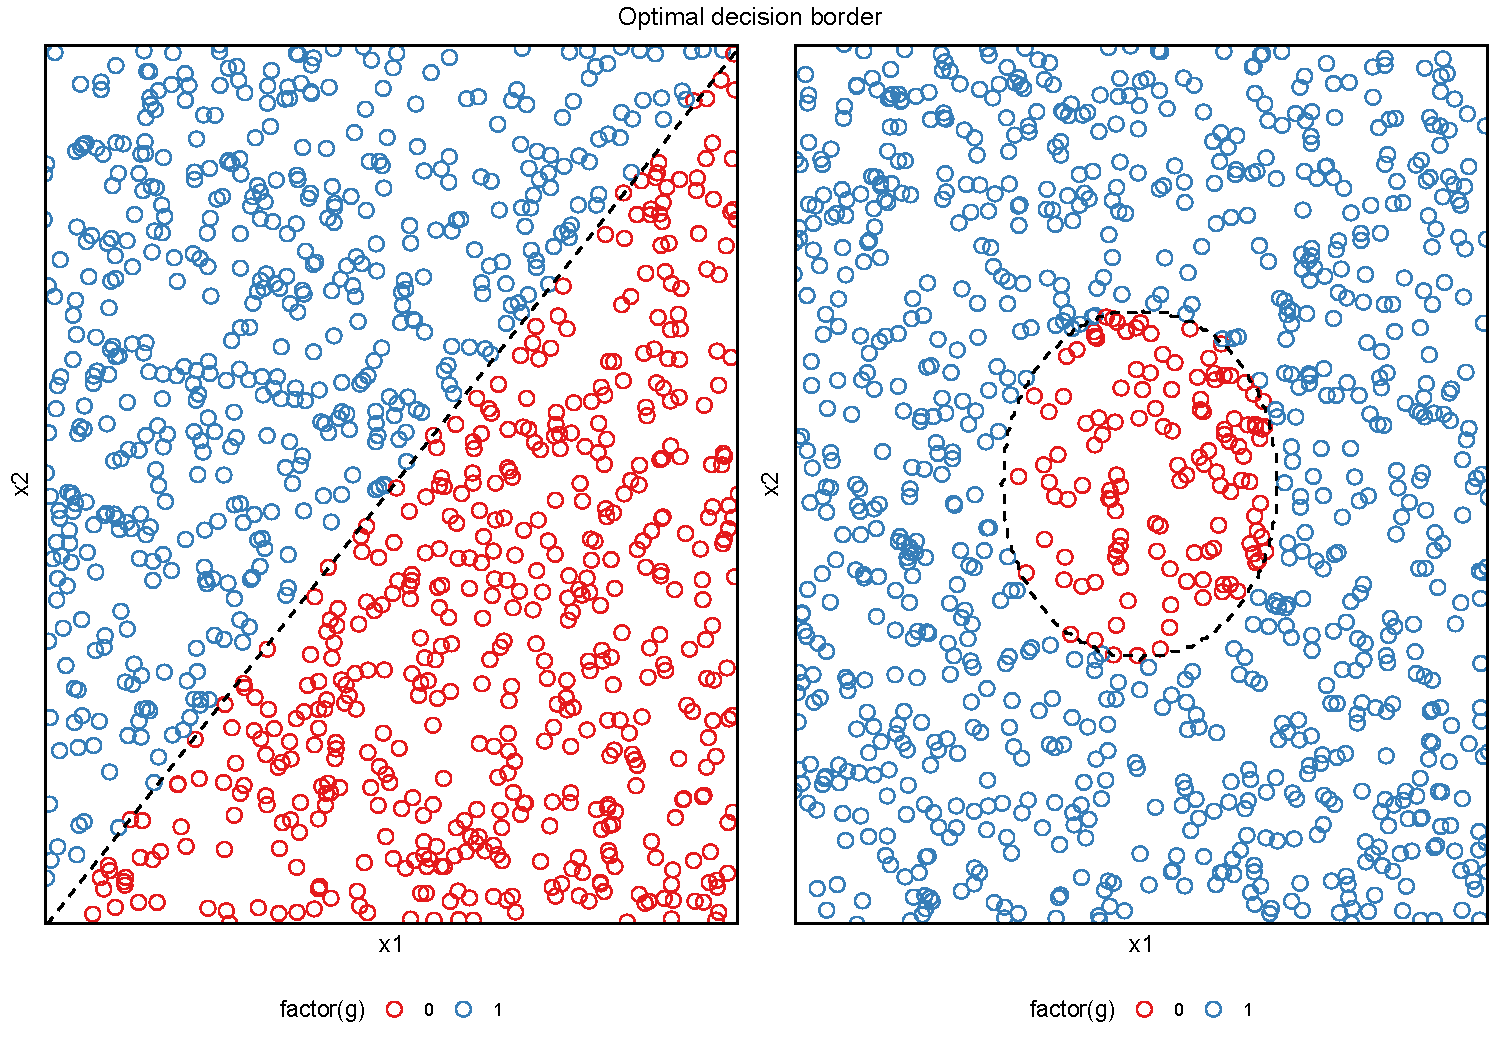
\includegraphics{_main_files/figure-beamer/unnamed-chunk-65-1} \end{center}
\end{block}

\begin{block}{Model fitting}
\protect\hypertarget{model-fitting-4}{}
Lorem ipsum dolor sit amet, consectetur adipiscing elit. Duis eu dictum lorem, et placerat dui. Donec porttitor posuere nisi, non tempor tellus ornare ut. Vestibulum vehicula libero eget consequat lobortis. Suspendisse vel arcu et urna iaculis mattis. Nulla ut mattis est. Pellentesque eu eleifend augue. Maecenas placerat tortor tincidunt risus rutrum tincidunt.

\begin{verbatim}
## Warning: The `...` are not used in this function but one or more objects were passed: 'verbose'
## The `...` are not used in this function but one or more objects were passed: 'verbose'
\end{verbatim}

\begin{verbatim}
##  Setting default kernel parameters
\end{verbatim}

\begin{verbatim}
## Warning: The `...` are not used in this function but one or more objects were passed: 'verbose'
## The `...` are not used in this function but one or more objects were passed: 'verbose'
\end{verbatim}

\begin{verbatim}
##  Setting default kernel parameters  
## maximum number of iterations reached 0.0006068825 -0.0006062308
\end{verbatim}
\end{block}

\begin{block}{Compare results}
\protect\hypertarget{compare-results-4}{}
The plots below show the resulting decision boundaries

\begin{verbatim}
## Warning: stat_contour(): Zero contours were generated
\end{verbatim}

\begin{verbatim}
## Warning in min(x): no non-missing arguments to min; returning Inf
\end{verbatim}

\begin{verbatim}
## Warning in max(x): no non-missing arguments to max; returning -Inf
\end{verbatim}

\begin{center}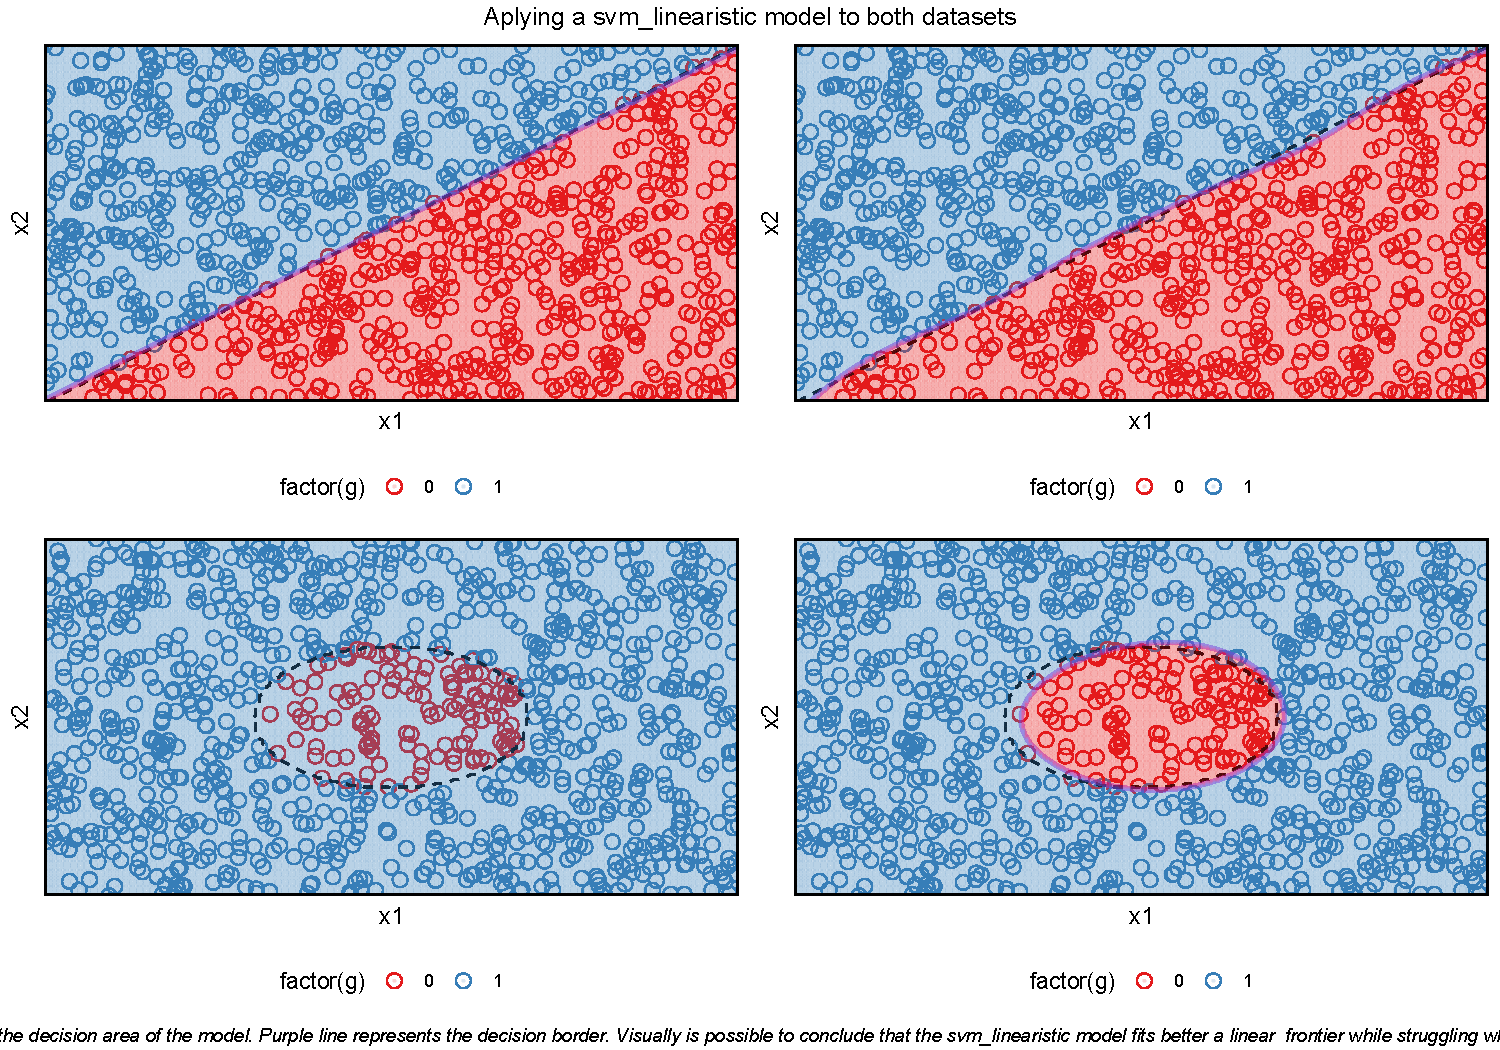
\includegraphics{_main_files/figure-beamer/unnamed-chunk-70-1} \end{center}

The plots shows the evolution of key metrics over crossvalidation trainning

\begin{center}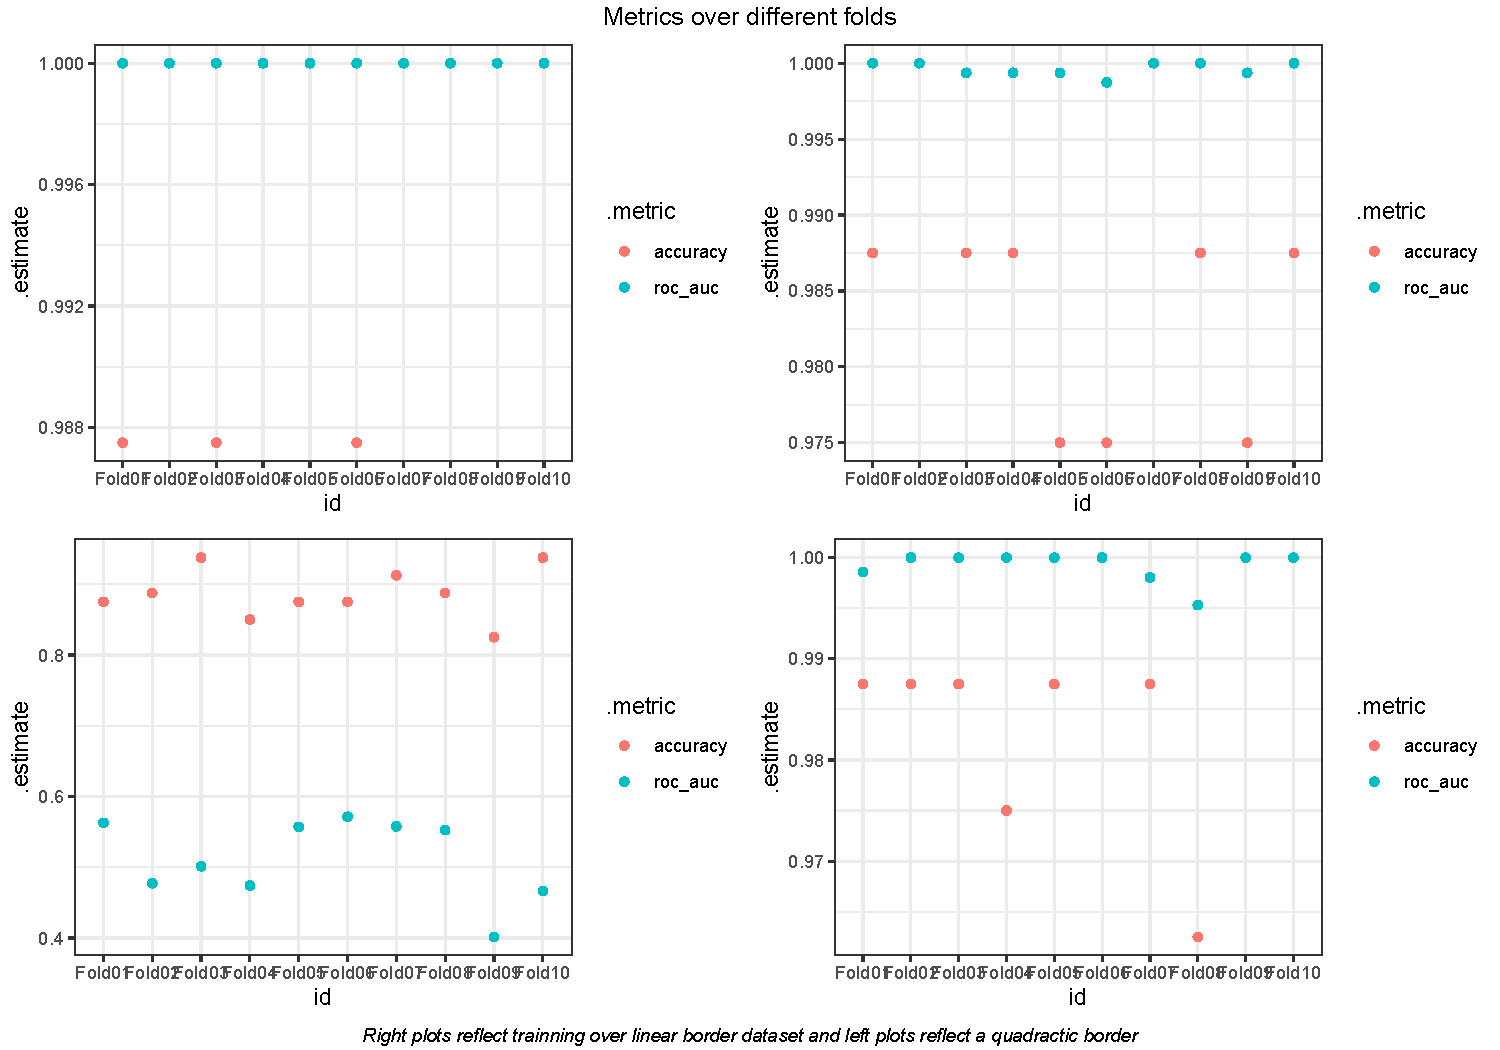
\includegraphics{_main_files/figure-beamer/unnamed-chunk-71-1} \end{center}

The plots show the metrics between different models

\begin{center}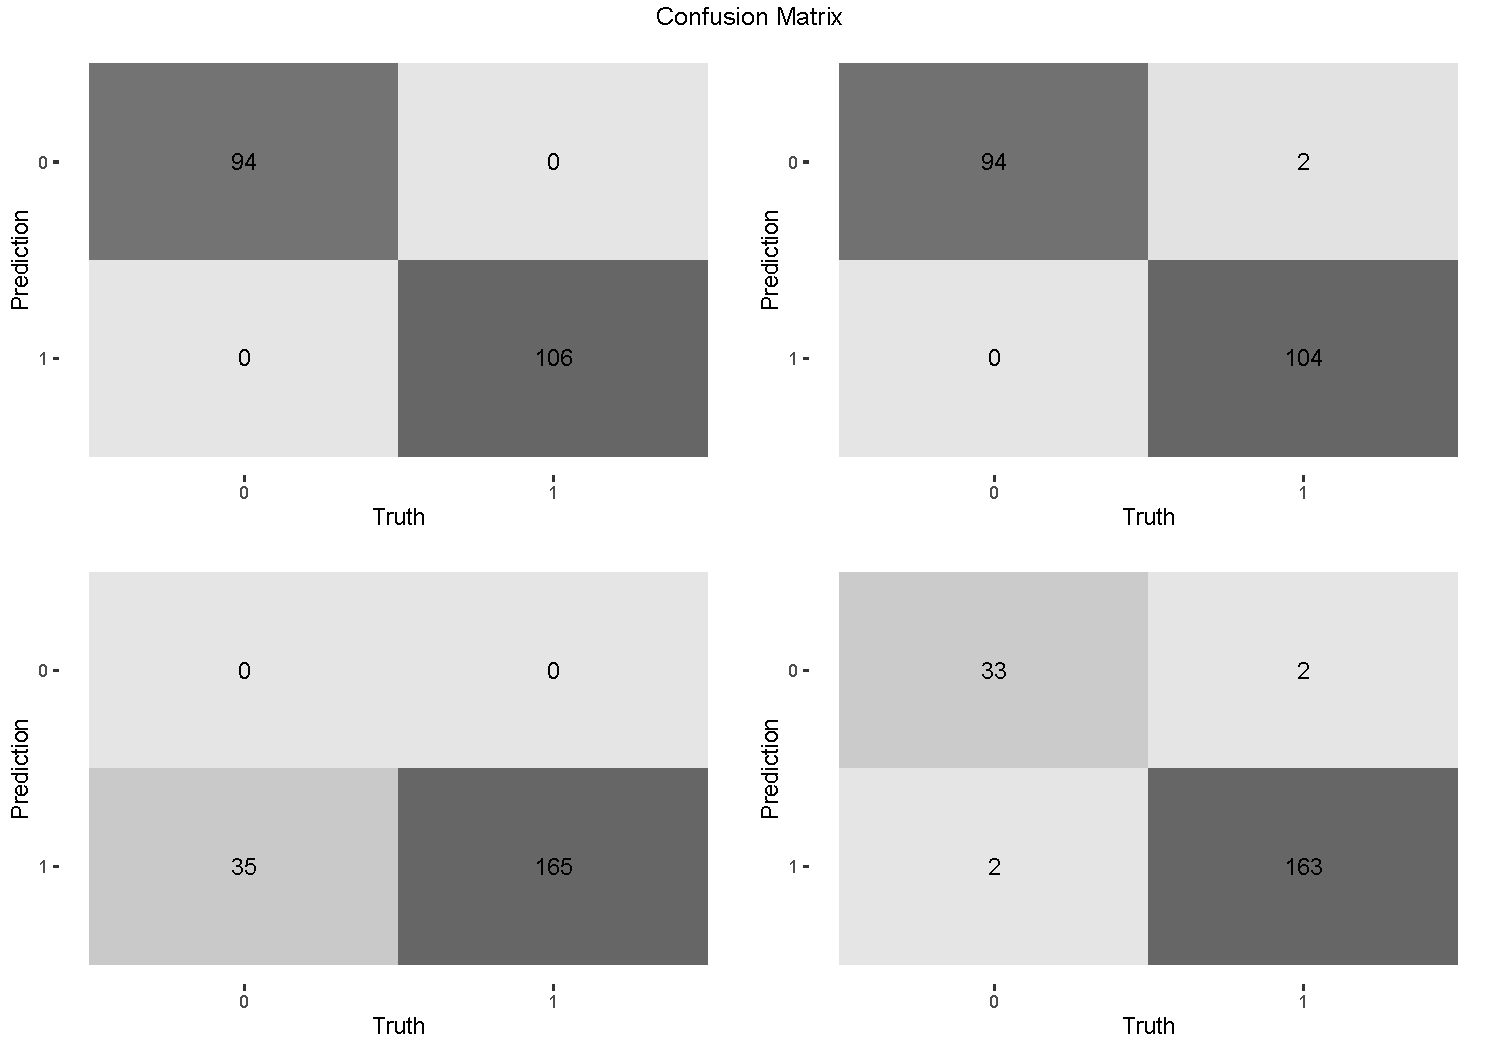
\includegraphics{_main_files/figure-beamer/unnamed-chunk-72-1} \end{center}

\begin{center}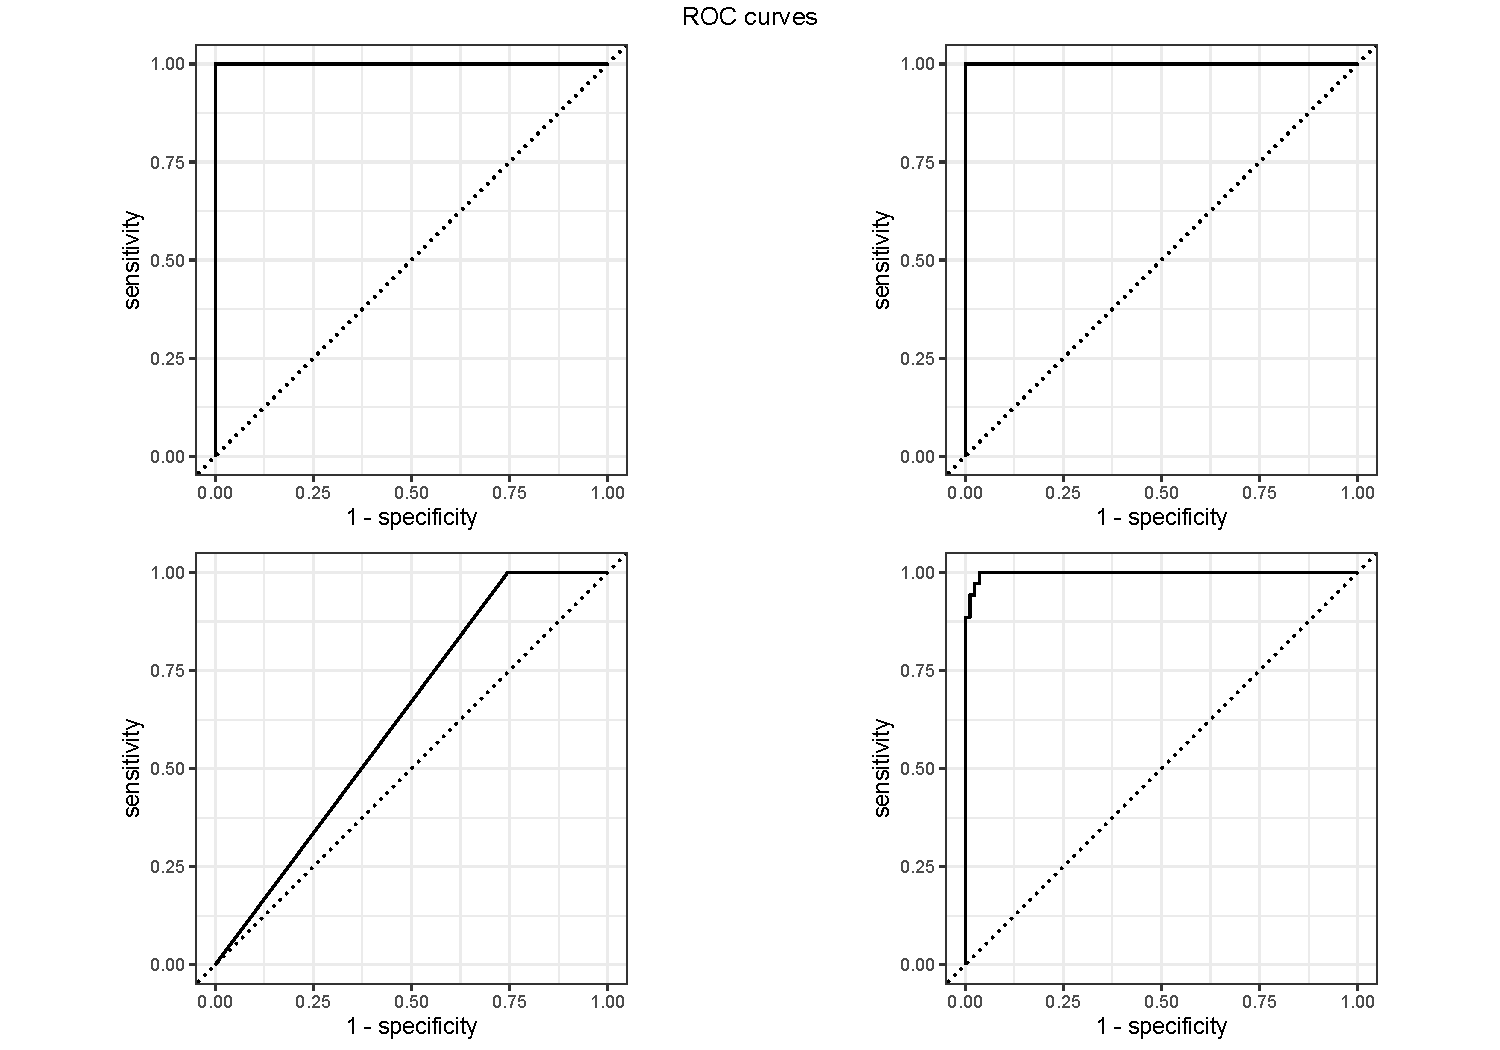
\includegraphics{_main_files/figure-beamer/unnamed-chunk-73-1} \end{center}
\end{block}

\begin{block}{Conclusion}
\protect\hypertarget{conclusion-4}{}
Lorem ipsum dolor sit amet, consectetur adipiscing elit. Duis eu dictum lorem, et placerat dui. Donec porttitor posuere nisi, non tempor tellus ornare ut. Vestibulum vehicula libero eget consequat lobortis. Suspendisse vel arcu et urna iaculis mattis. Nulla ut mattis est. Pellentesque eu eleifend augue. Maecenas placerat tortor tincidunt risus rutrum tincidunt.
\end{block}
\end{frame}

\begin{frame}[fragile]{SVM Radial vs SVM linear}
\protect\hypertarget{svm-radial-vs-svm-linear-1}{}
\begin{block}{Dataset definition}
\protect\hypertarget{dataset-definition-5}{}
Lorem ipsum dolor sit amet, consectetur adipiscing elit. Duis eu dictum lorem, et placerat dui. Donec porttitor posuere nisi, non tempor tellus ornare ut. Vestibulum vehicula libero eget consequat lobortis. Suspendisse vel arcu et urna iaculis mattis. Nulla ut mattis est. Pellentesque eu eleifend augue. Maecenas placerat tortor tincidunt risus rutrum tincidunt.

\begin{center}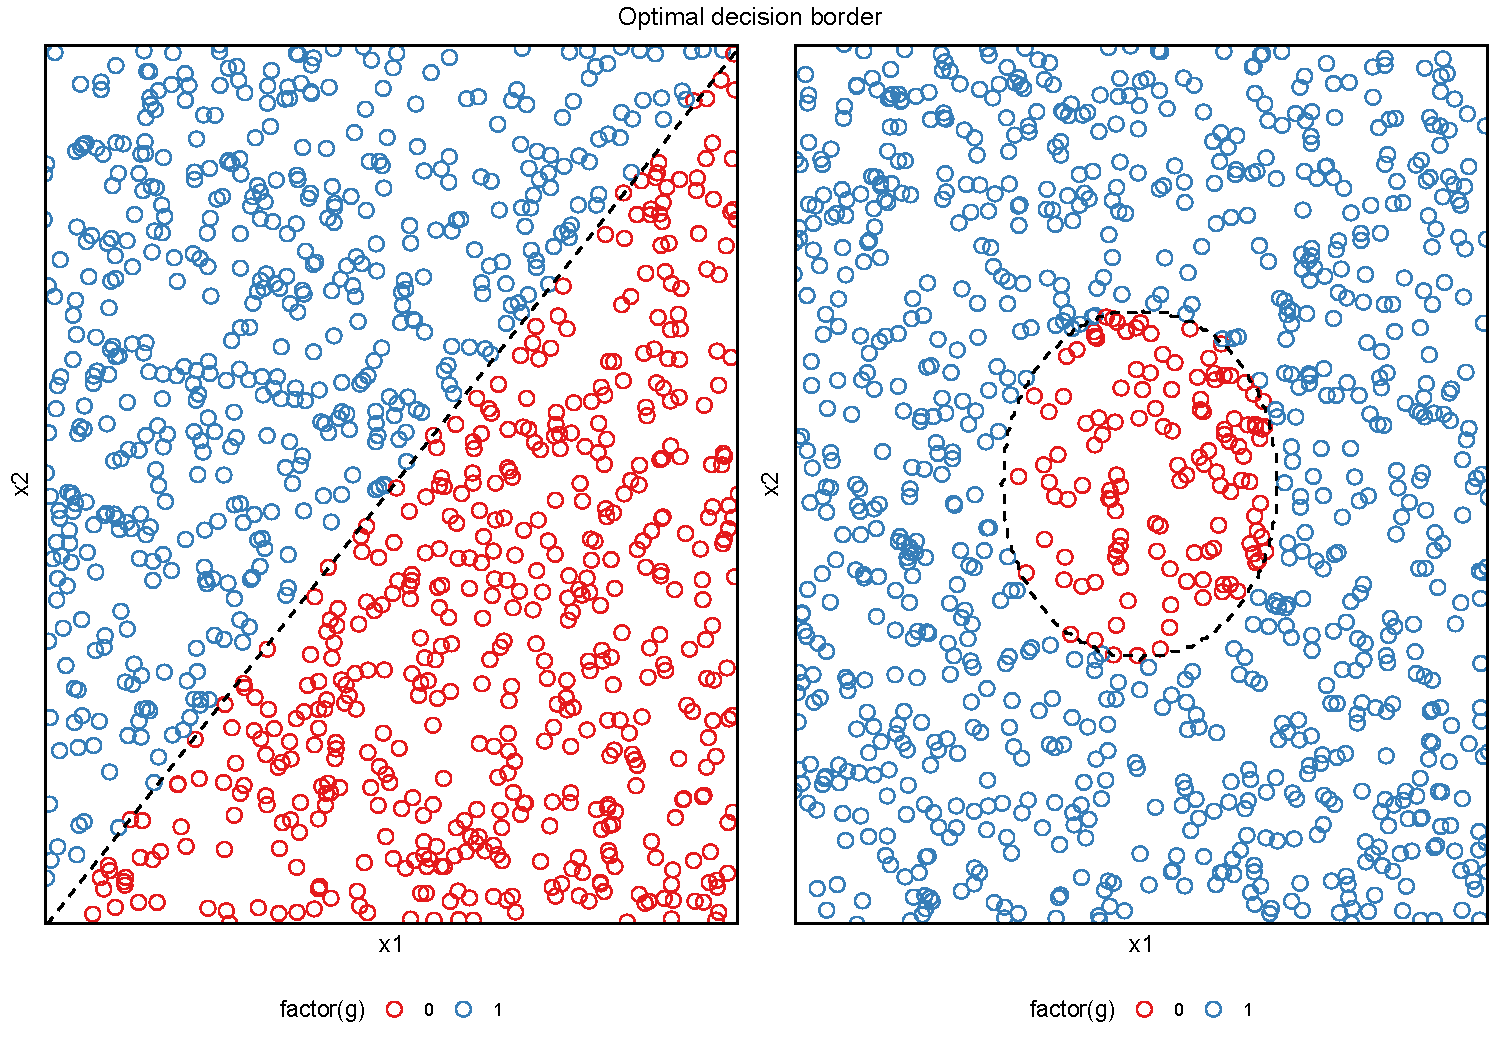
\includegraphics{_main_files/figure-beamer/unnamed-chunk-77-1} \end{center}
\end{block}

\begin{block}{Model fitting}
\protect\hypertarget{model-fitting-5}{}
Lorem ipsum dolor sit amet, consectetur adipiscing elit. Duis eu dictum lorem, et placerat dui. Donec porttitor posuere nisi, non tempor tellus ornare ut. Vestibulum vehicula libero eget consequat lobortis. Suspendisse vel arcu et urna iaculis mattis. Nulla ut mattis est. Pellentesque eu eleifend augue. Maecenas placerat tortor tincidunt risus rutrum tincidunt.

\begin{verbatim}
## Warning: The `...` are not used in this function but one or more objects were passed: 'verbose'
## The `...` are not used in this function but one or more objects were passed: 'verbose'
\end{verbatim}

\begin{verbatim}
##  Setting default kernel parameters
\end{verbatim}

\begin{verbatim}
## Warning: The `...` are not used in this function but one or more objects were passed: 'verbose'
## The `...` are not used in this function but one or more objects were passed: 'verbose'
\end{verbatim}

\begin{verbatim}
##  Setting default kernel parameters  
## maximum number of iterations reached 0.0006068825 -0.0006062308
\end{verbatim}
\end{block}

\begin{block}{Compare results}
\protect\hypertarget{compare-results-5}{}
The plots below show the resulting decision boundaries

\begin{verbatim}
## Warning: stat_contour(): Zero contours were generated
\end{verbatim}

\begin{verbatim}
## Warning in min(x): no non-missing arguments to min; returning Inf
\end{verbatim}

\begin{verbatim}
## Warning in max(x): no non-missing arguments to max; returning -Inf
\end{verbatim}

\begin{center}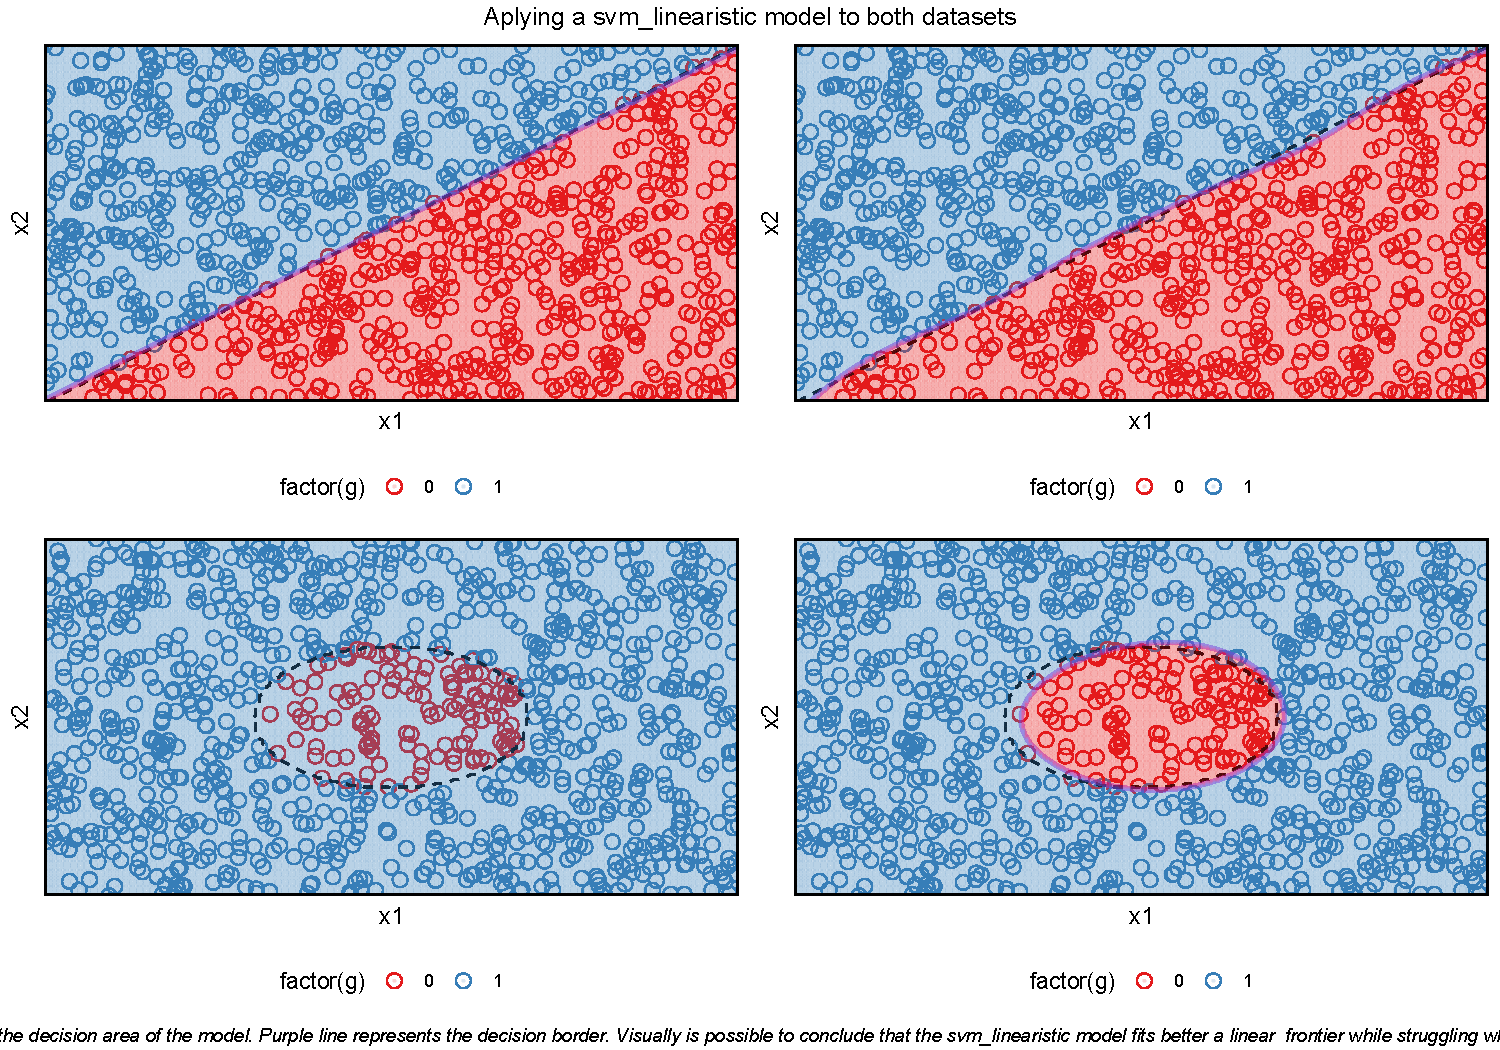
\includegraphics{_main_files/figure-beamer/unnamed-chunk-82-1} \end{center}

The plots shows the evolution of key metrics over crossvalidation trainning

\begin{center}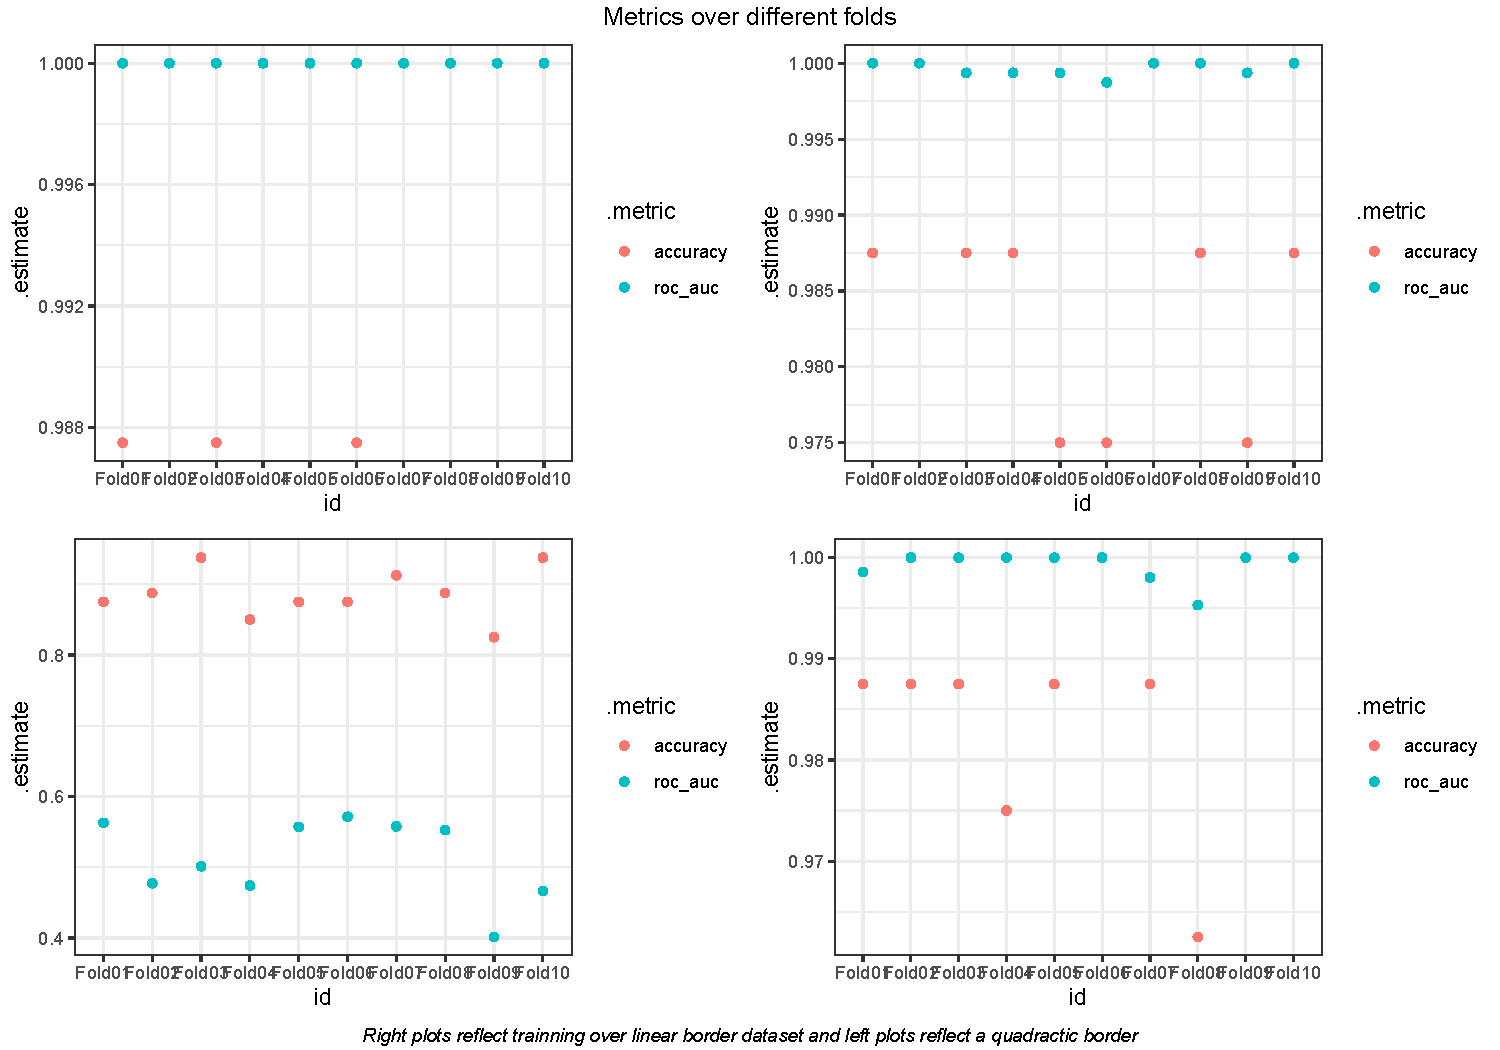
\includegraphics{_main_files/figure-beamer/unnamed-chunk-83-1} \end{center}

The plots show the metrics between different models

\begin{center}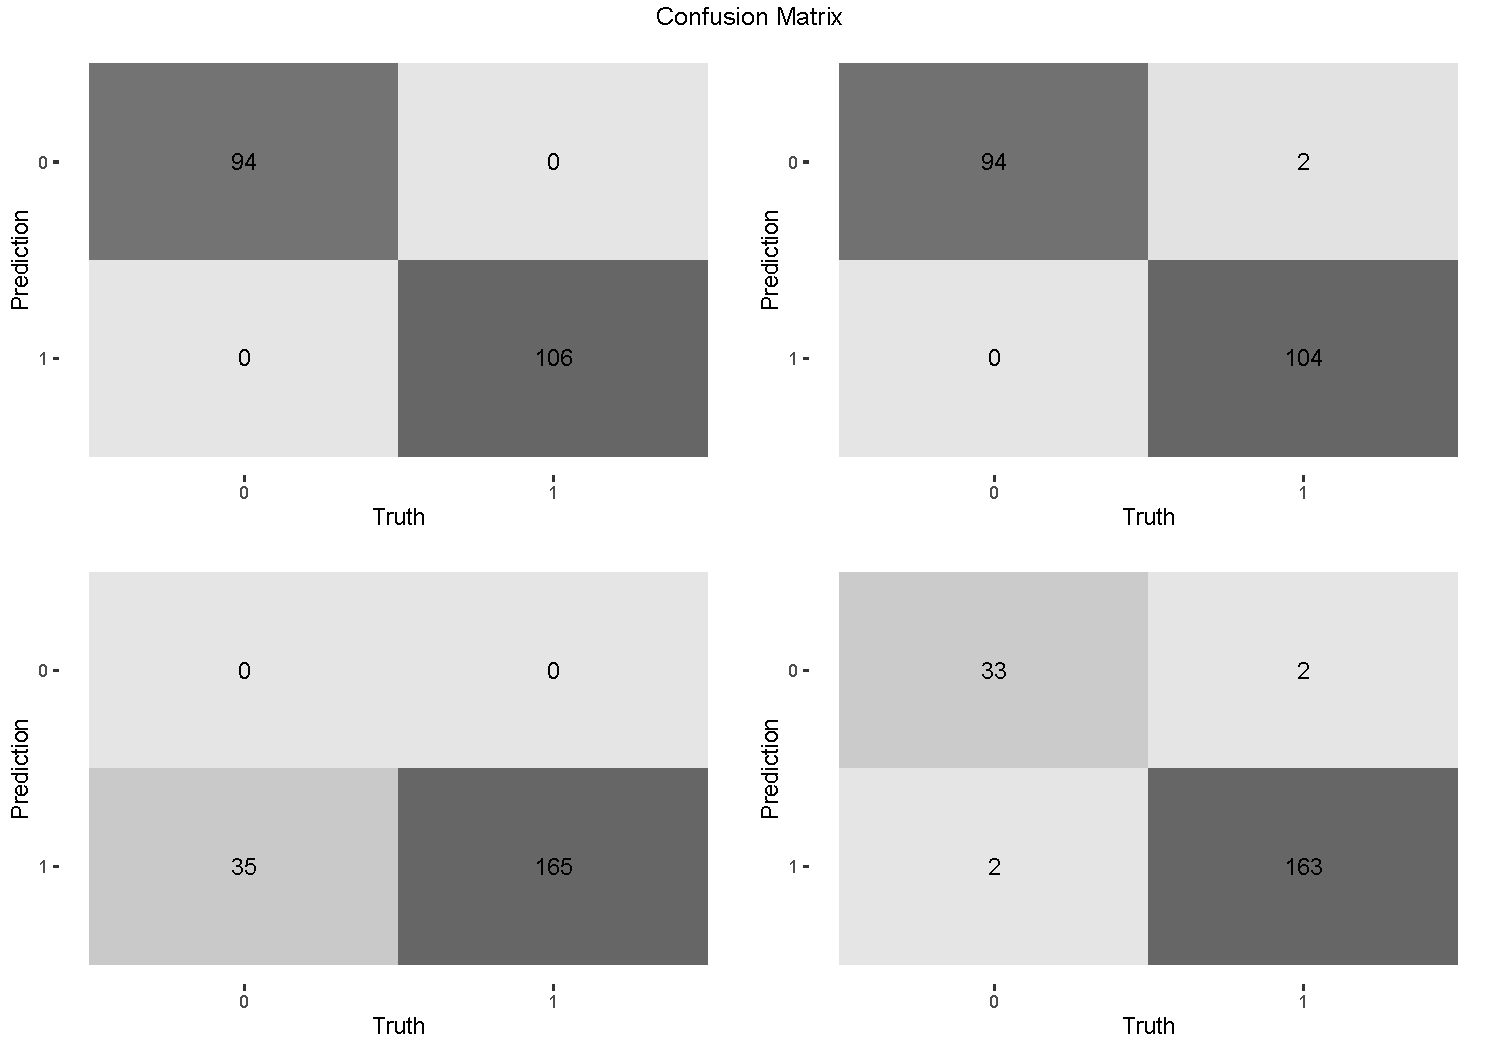
\includegraphics{_main_files/figure-beamer/unnamed-chunk-84-1} \end{center}

\begin{center}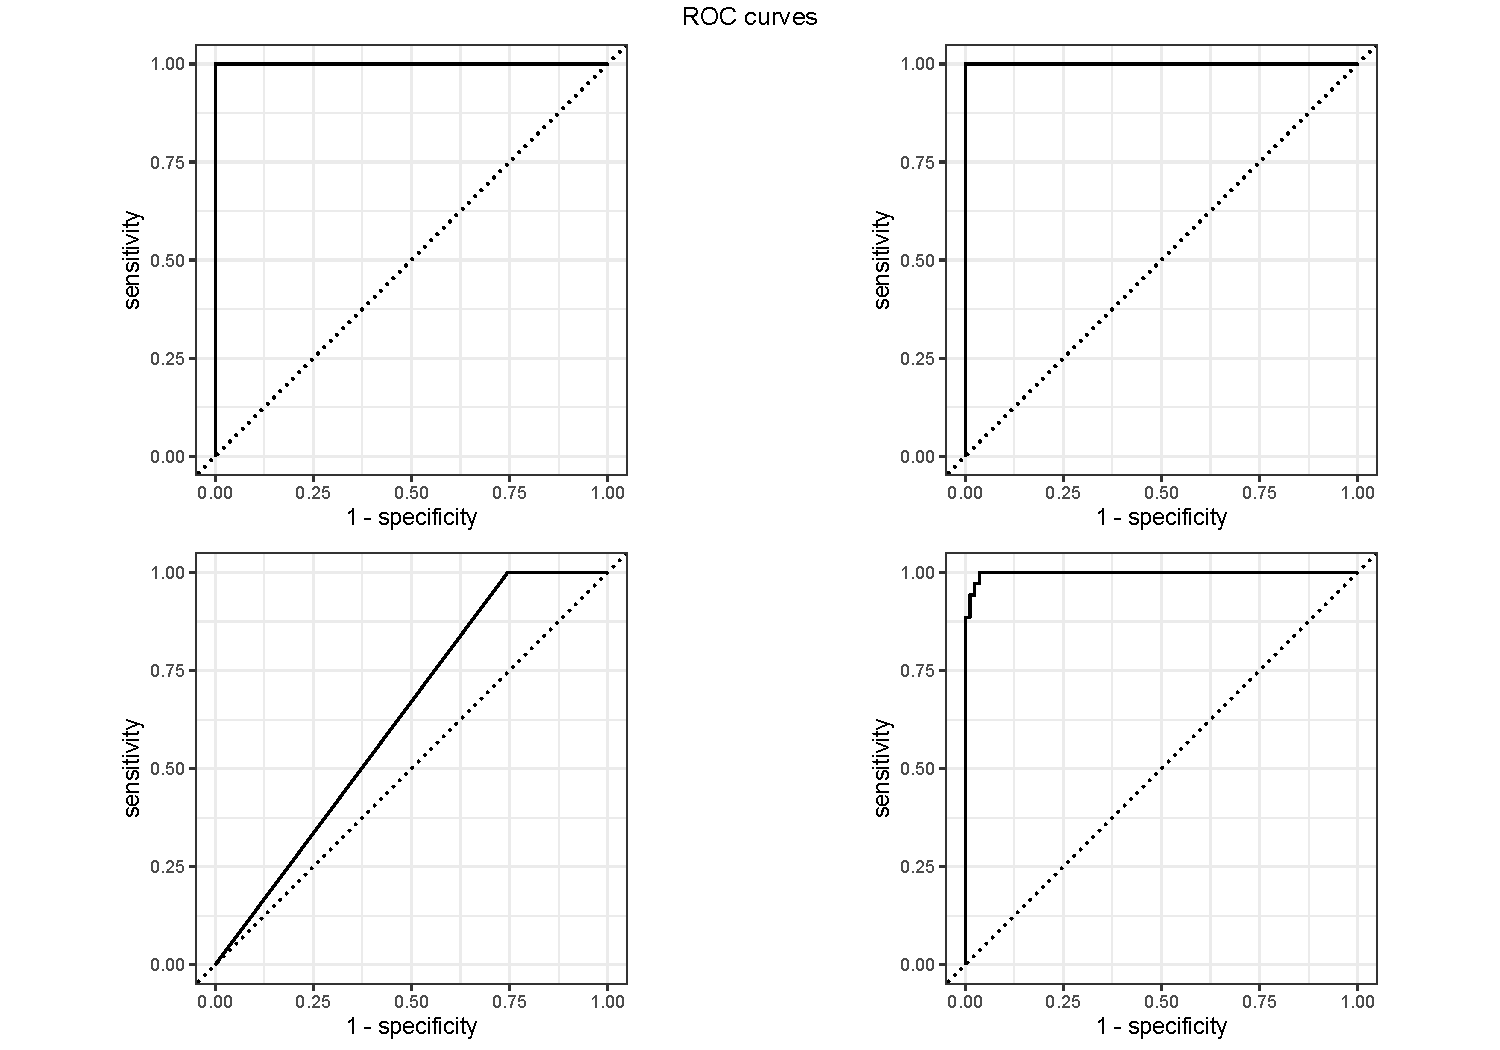
\includegraphics{_main_files/figure-beamer/unnamed-chunk-85-1} \end{center}
\end{block}

\begin{block}{Conclusion}
\protect\hypertarget{conclusion-5}{}
Lorem ipsum dolor sit amet, consectetur adipiscing elit. Duis eu dictum lorem, et placerat dui. Donec porttitor posuere nisi, non tempor tellus ornare ut. Vestibulum vehicula libero eget consequat lobortis. Suspendisse vel arcu et urna iaculis mattis. Nulla ut mattis est. Pellentesque eu eleifend augue. Maecenas placerat tortor tincidunt risus rutrum tincidunt.
\end{block}
\end{frame}

\begin{frame}[fragile]{MLP vs knn}
\protect\hypertarget{mlp-vs-knn}{}
\begin{block}{Dataset definition}
\protect\hypertarget{dataset-definition-6}{}
Lorem ipsum dolor sit amet, consectetur adipiscing elit. Duis eu dictum lorem, et placerat dui. Donec porttitor posuere nisi, non tempor tellus ornare ut. Vestibulum vehicula libero eget consequat lobortis. Suspendisse vel arcu et urna iaculis mattis. Nulla ut mattis est. Pellentesque eu eleifend augue. Maecenas placerat tortor tincidunt risus rutrum tincidunt.

\begin{center}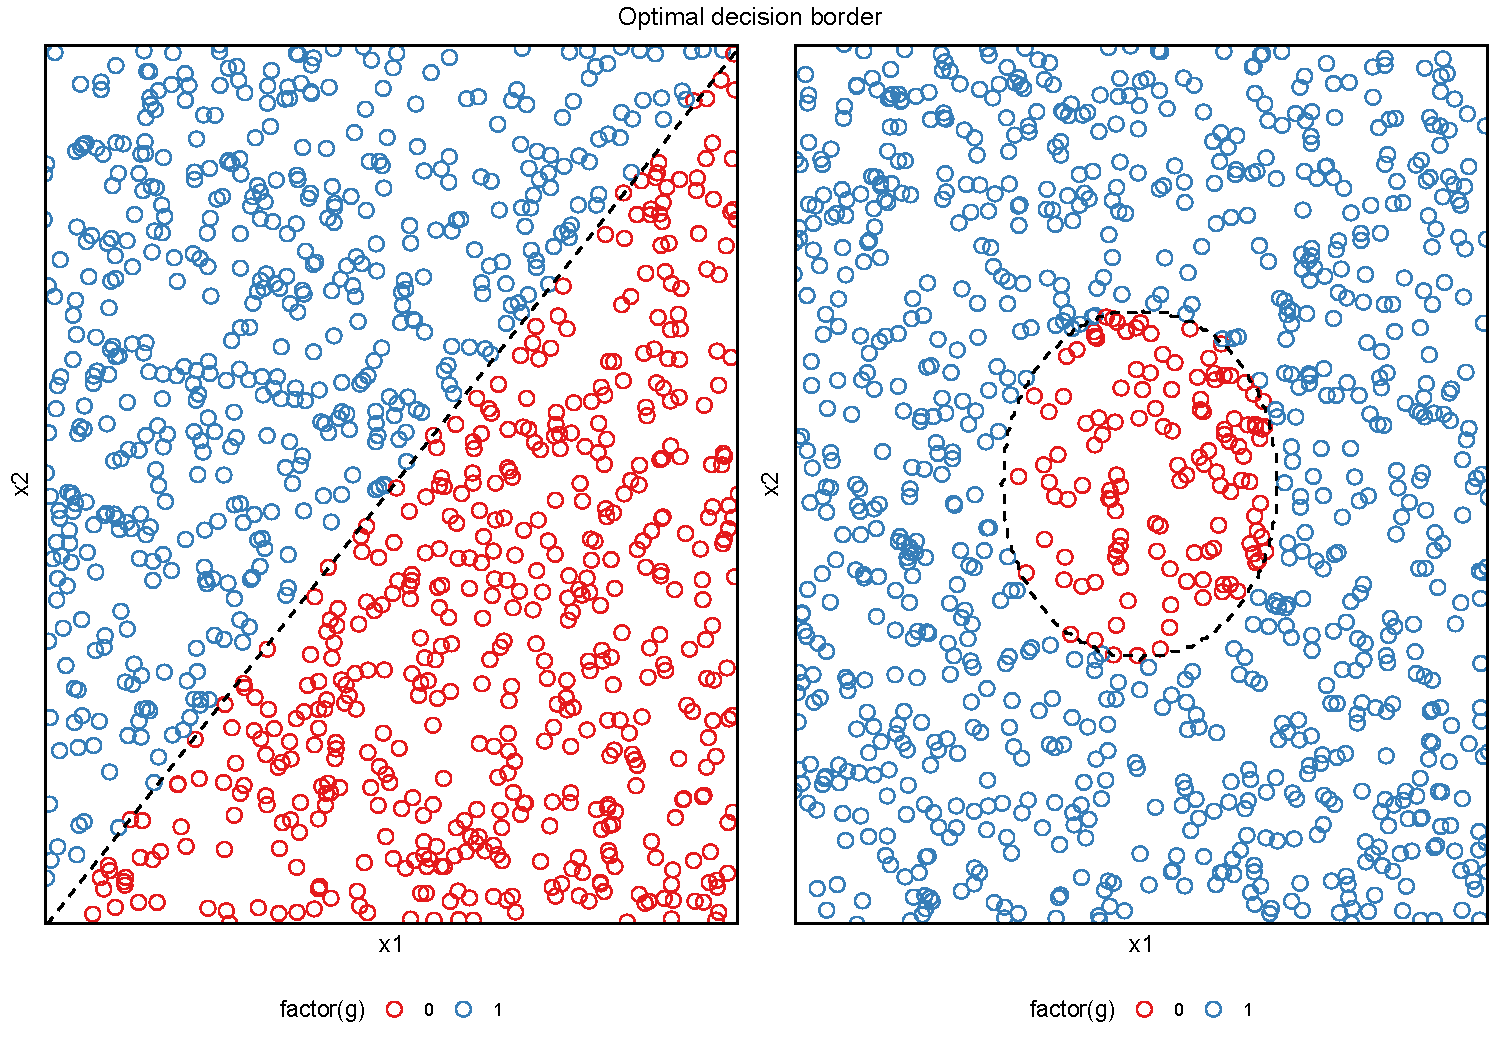
\includegraphics{_main_files/figure-beamer/unnamed-chunk-89-1} \end{center}
\end{block}

\begin{block}{Model fitting}
\protect\hypertarget{model-fitting-6}{}
Lorem ipsum dolor sit amet, consectetur adipiscing elit. Duis eu dictum lorem, et placerat dui. Donec porttitor posuere nisi, non tempor tellus ornare ut. Vestibulum vehicula libero eget consequat lobortis. Suspendisse vel arcu et urna iaculis mattis. Nulla ut mattis est. Pellentesque eu eleifend augue. Maecenas placerat tortor tincidunt risus rutrum tincidunt.

\begin{verbatim}
## Warning: The `...` are not used in this function but one or more objects were passed: 'verbose'
## The `...` are not used in this function but one or more objects were passed: 'verbose'
## The `...` are not used in this function but one or more objects were passed: 'verbose'
## The `...` are not used in this function but one or more objects were passed: 'verbose'
\end{verbatim}
\end{block}

\begin{block}{Compare results}
\protect\hypertarget{compare-results-6}{}
The plots below show the resulting decision boundaries

\begin{verbatim}
## Warning: stat_contour(): Zero contours were generated
\end{verbatim}

\begin{verbatim}
## Warning in min(x): no non-missing arguments to min; returning Inf
\end{verbatim}

\begin{verbatim}
## Warning in max(x): no non-missing arguments to max; returning -Inf
\end{verbatim}

\begin{center}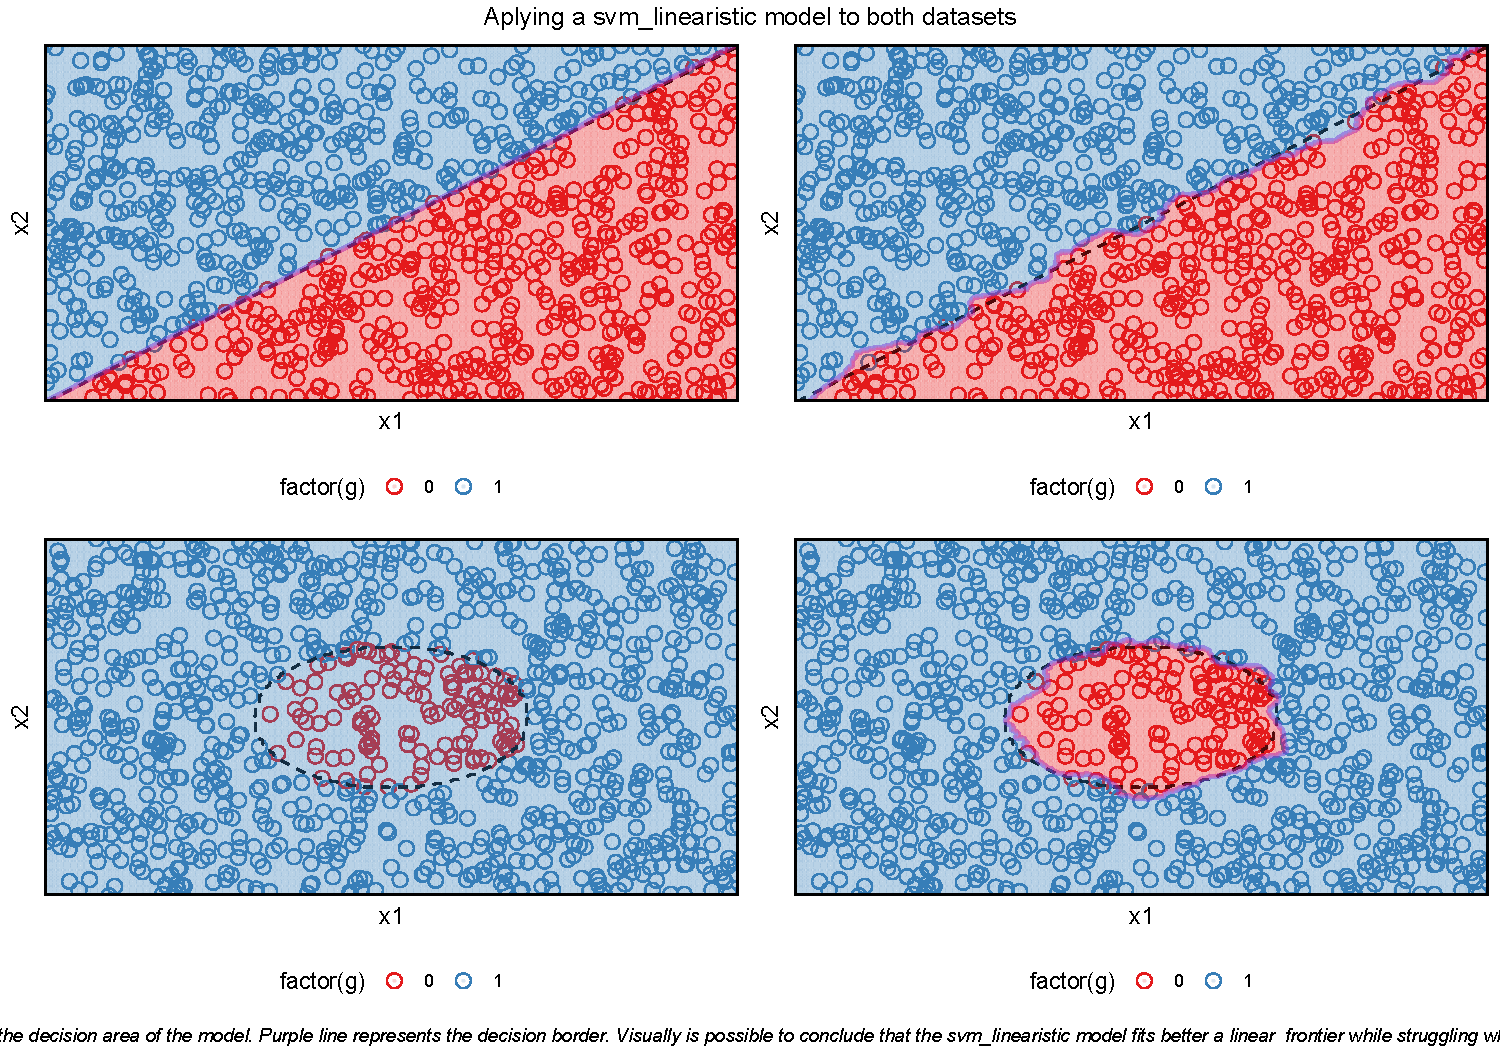
\includegraphics{_main_files/figure-beamer/unnamed-chunk-94-1} \end{center}

The plots shows the evolution of key metrics over crossvalidation trainning

\begin{center}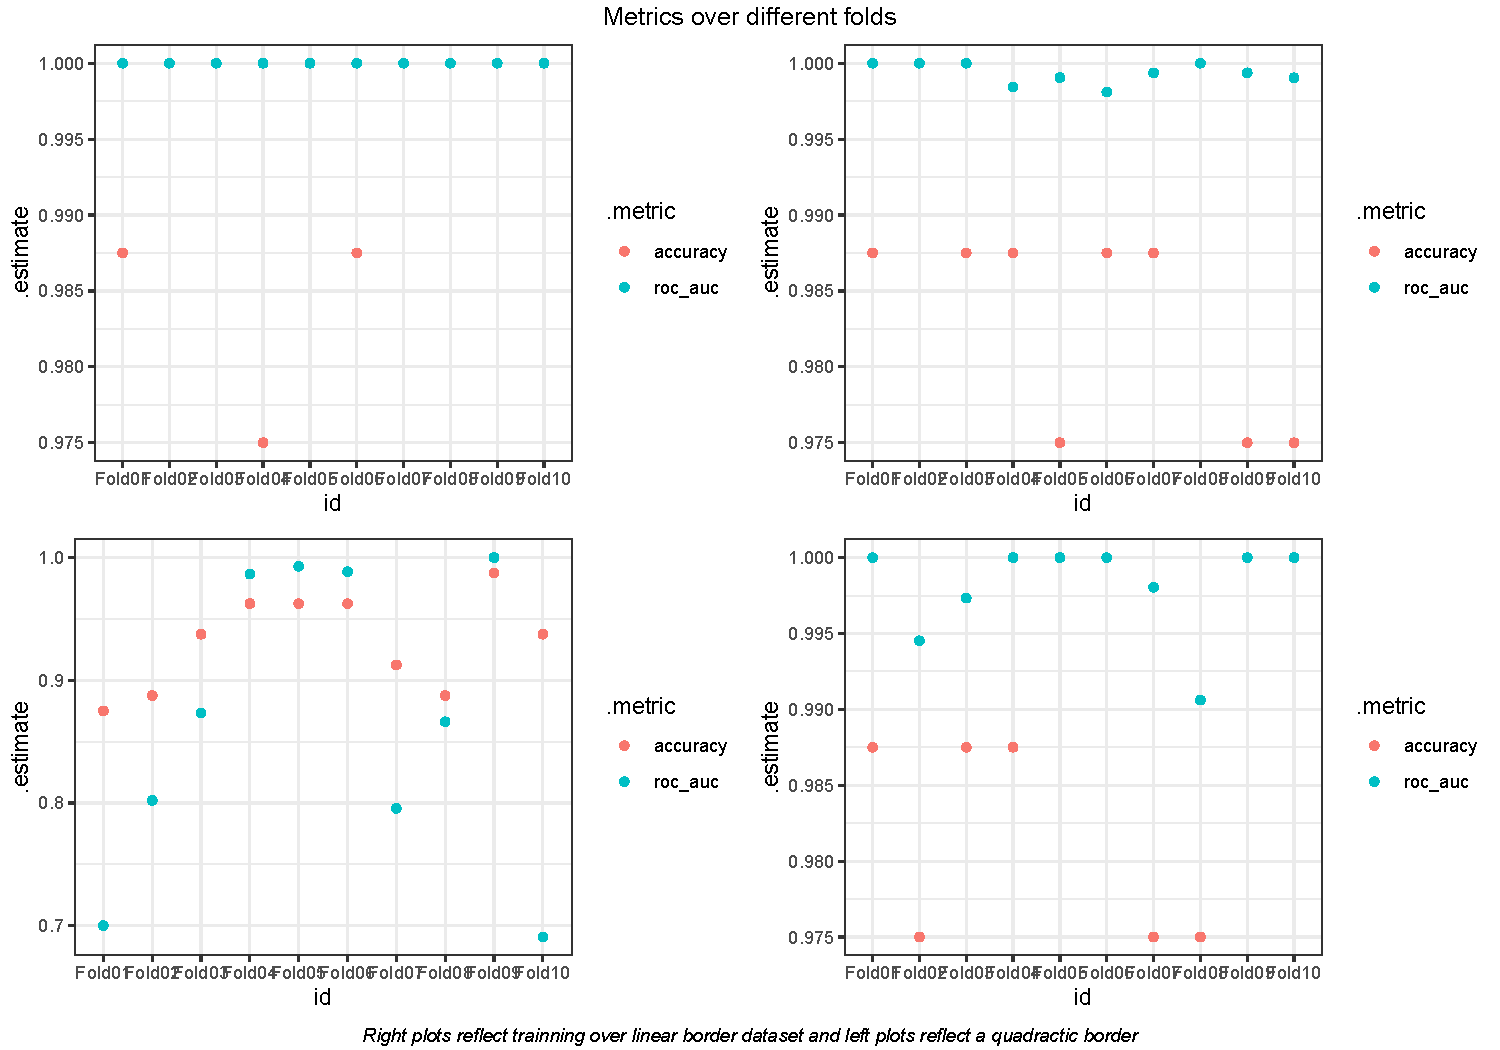
\includegraphics{_main_files/figure-beamer/unnamed-chunk-95-1} \end{center}

The plots show the metrics between different models

\begin{center}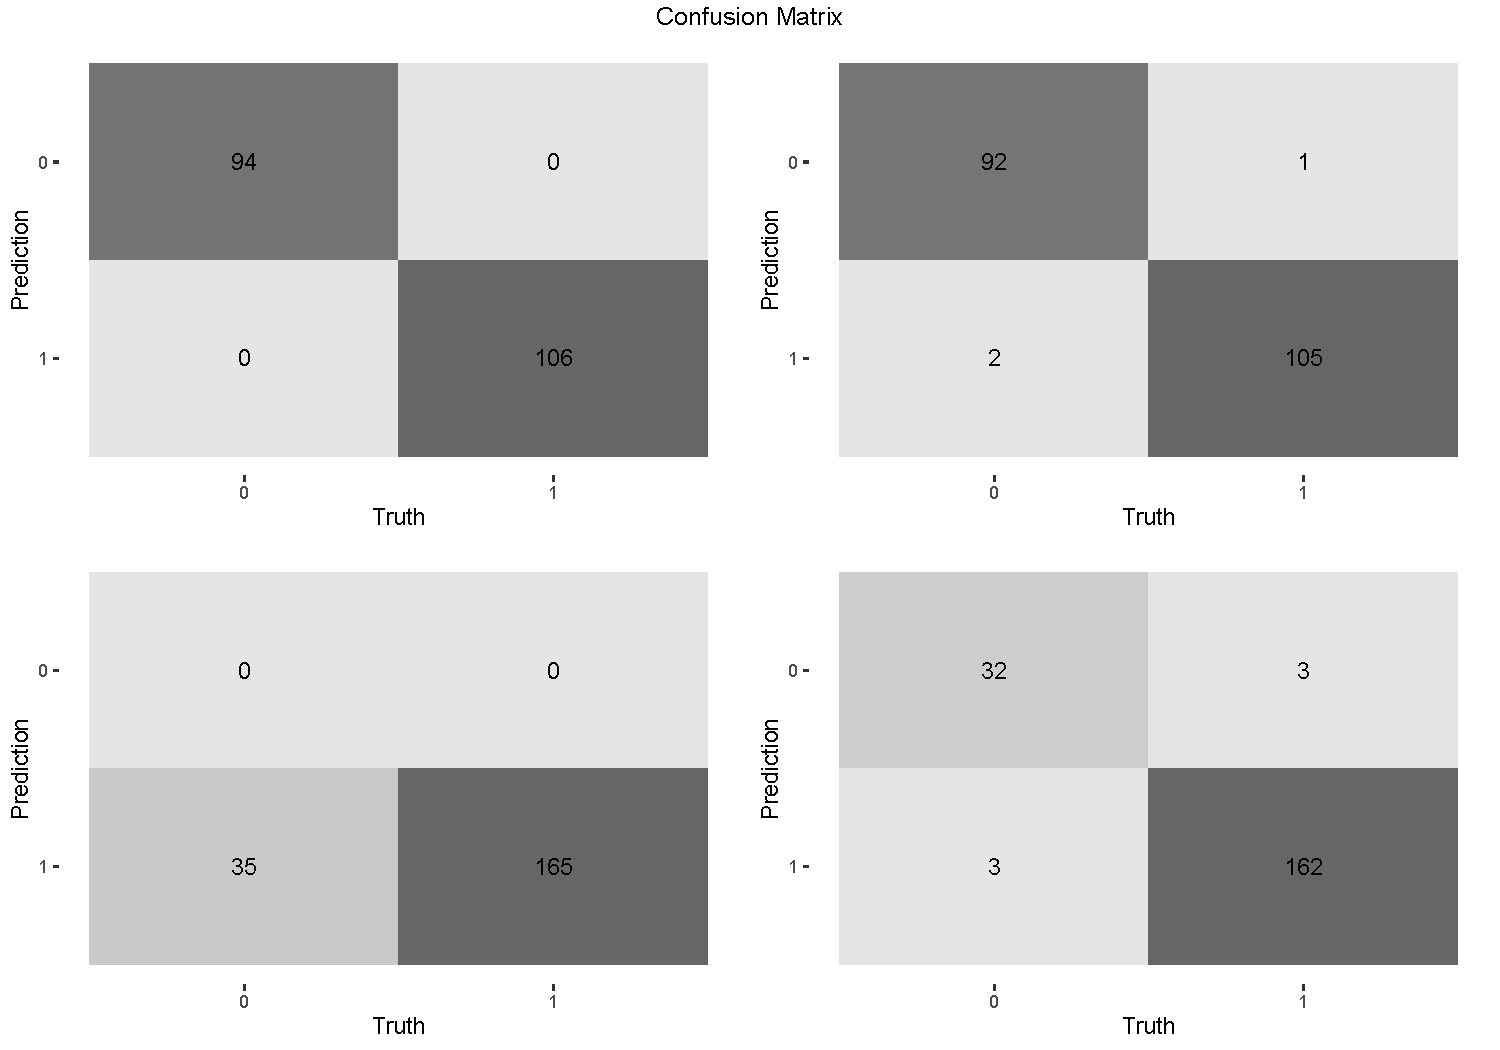
\includegraphics{_main_files/figure-beamer/unnamed-chunk-96-1} \end{center}

\begin{center}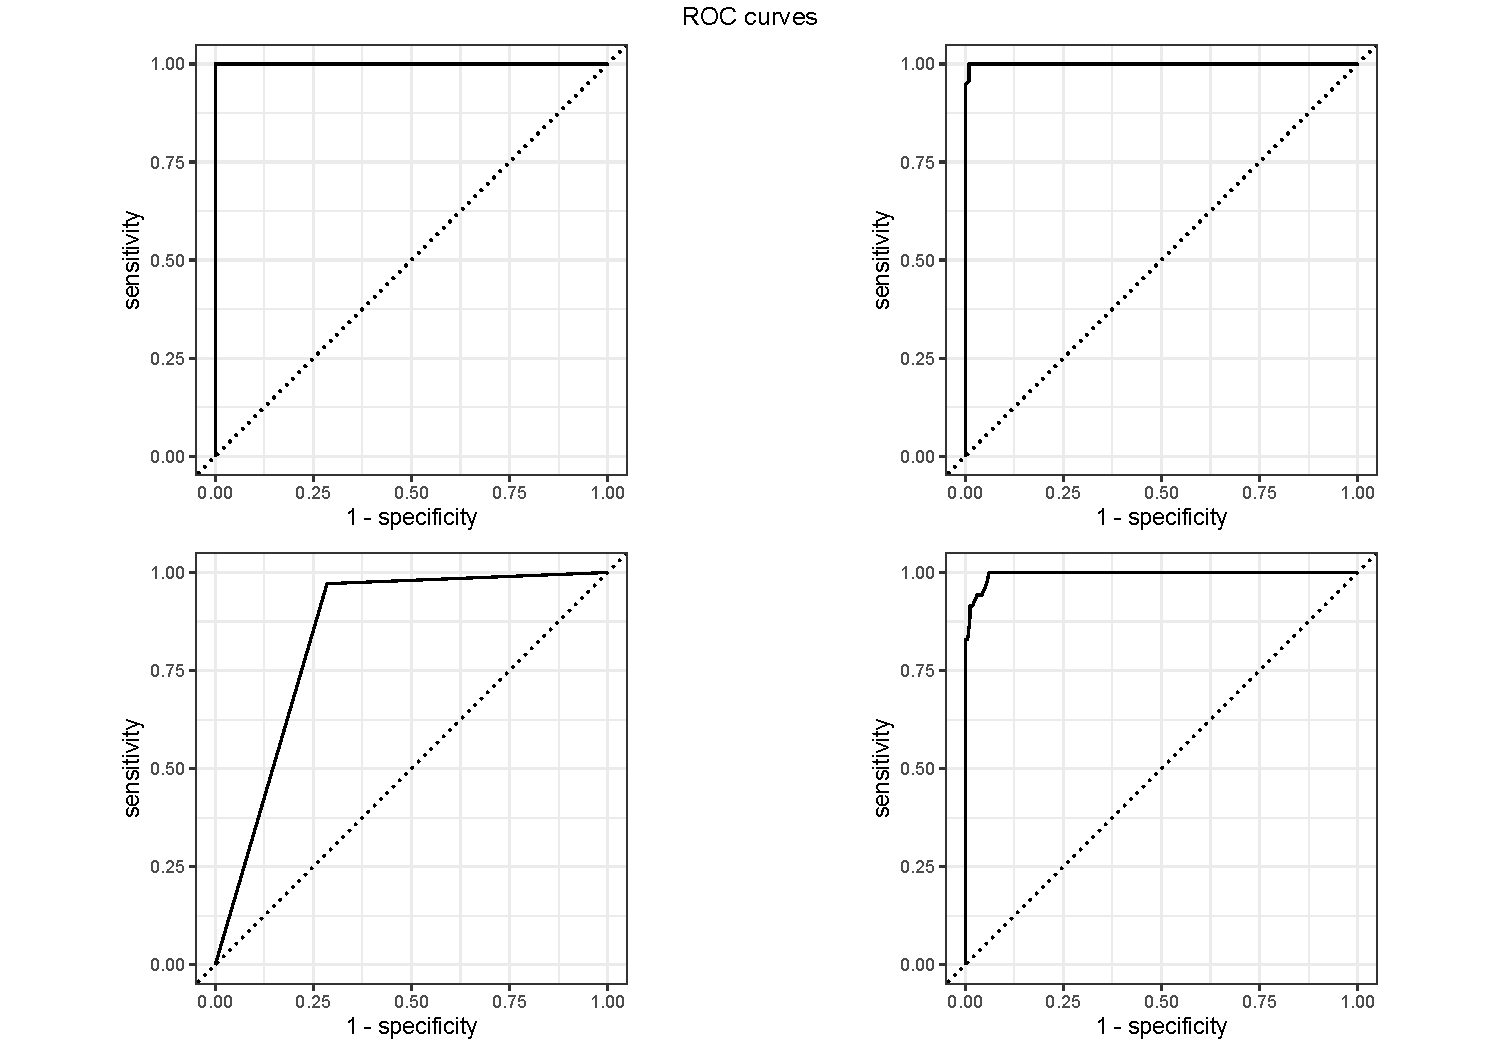
\includegraphics{_main_files/figure-beamer/unnamed-chunk-97-1} \end{center}
\end{block}

\begin{block}{Conclusion}
\protect\hypertarget{conclusion-6}{}
Lorem ipsum dolor sit amet, consectetur adipiscing elit. Duis eu dictum lorem, et placerat dui. Donec porttitor posuere nisi, non tempor tellus ornare ut. Vestibulum vehicula libero eget consequat lobortis. Suspendisse vel arcu et urna iaculis mattis. Nulla ut mattis est. Pellentesque eu eleifend augue. Maecenas placerat tortor tincidunt risus rutrum tincidunt.
\end{block}

\begin{block}{Plot}
\protect\hypertarget{plot}{}
See Figure \ref{fig:foo}.

\begin{figure}

{\centering 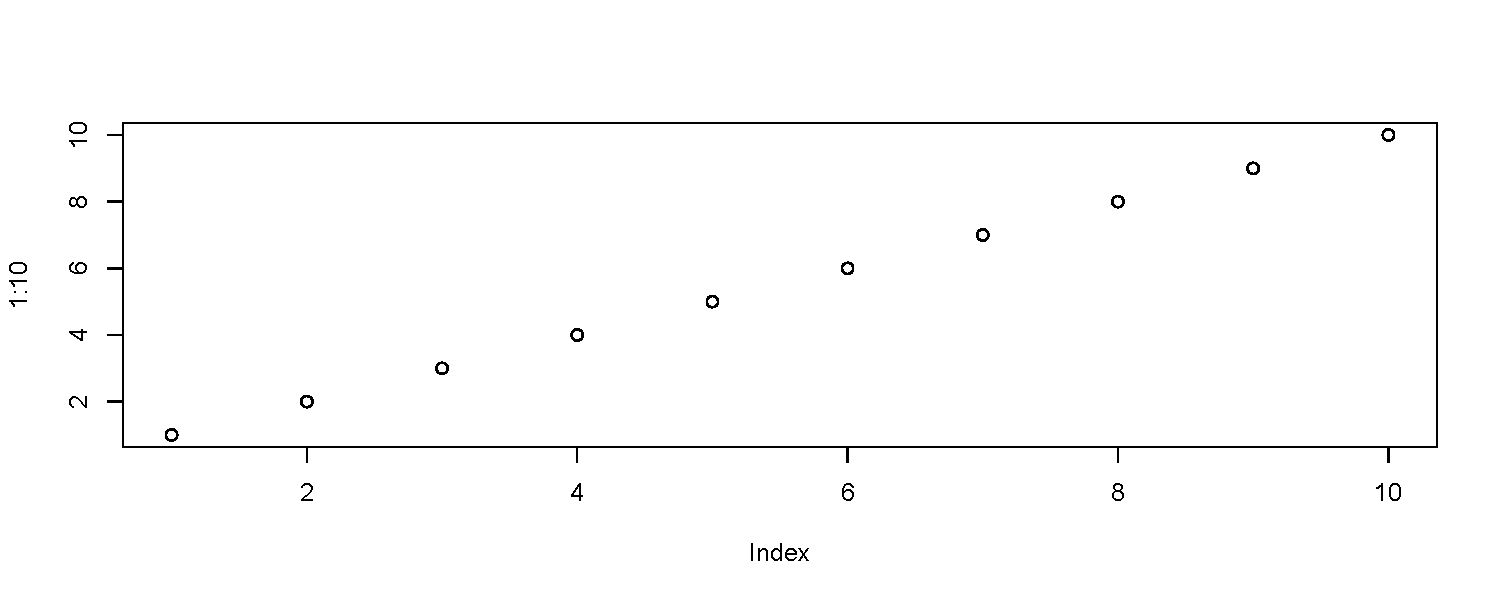
\includegraphics{_main_files/figure-beamer/foo-1} 

}

\caption{Hi there}\label{fig:foo}
\end{figure}
\end{block}
\end{frame}

\end{document}
